% ; whizzy -pdf .
%                                      
%\documentclass[10pt,prof,handout]{beamer}    % Version de travail, avec tout dessus
%\documentclass[10pt,prof]{beamer}    % Version de travail, avec tout dessus
%\documentclass[10pt,handout]{beamer}% Version a imprimer, sans reponses ni contenu des trous
\documentclass[10pt]{beamer}        % Version a projeter, sans reponse avec contenu trous

% HOWTO: 
%  \trou{contenu des trous}
%  \ifprof{a ne jamais montrer aux etudiants (reponses?)}
%         {ce qu'ils doivent voir a la place (un trou pour ecrire)}
%  \only<beamer>{texte present que sur les slides de question (rarement utile)}
%  \only<handout>{todo}
  
%\usepackage[french]{babel}
\usepackage[utf8]{inputenc}
\usepackage{pdfpages}

\usepackage{beamerthemeEmptty3}

%\setbeamercovered{highly dynamic}
\setbeamertemplate{navigation symbols}[]
%\setbeamertemplate{section in toc}[ball unnumbered]
\setbeamertemplate{frametitle continuation}[from second][(suite)]

\usepackage{tikz,calc,ifthen}
\usetikzlibrary{decorations.pathmorphing,backgrounds,positioning,fit,arrows}
%placements,

\renewcommand{\sectionpagetitle}{Chapter \thepart}

\newcommand{\toc}{\mypartpageEN}
\newcommand{\subtoc}{\sectionpage}
\newcommand{\subsubtoc}{%
  \frame{%
    \frametitle{\hyperlink{end}{\agendatitle}}
    \tableofcontents[sectionstyle=show/shaded,%
                     subsectionstyle=show/shaded/shaded,%
                     subsubsectionstyle=show/hide/hide]
  }
}


%% drawSlice: dessine un pie-chart. 
%% Utilisé dans l'introduction
%%
\newcommand{\drawSlice}[5]{
  \pgfmathparse{0.5*#1+0.5*#2}
  \let\midangle\pgfmathresult
  
  % slice
  \draw[thick,fill=#5!30] (0,0) -- (#1:1) arc (#1:#2:1) -- cycle;
  
  % outer label
  \node[label=\midangle:#4] at (\midangle:1) {};
  
  % inner label
  \pgfmathparse{min((#2-#1-10)/110*(-0.3),0)}
  \let\temp\pgfmathresult
  \pgfmathparse{max(\temp,-0.5) + 0.8}
  \let\innerpos\pgfmathresult
  \node at (\midangle:\innerpos) {#3};
}


%%% Debut des hostilites
%%%

\newcommand{\n}{\textbackslash n}
\newcommand{\API}[1]{\colorbox{blue!25}{#1}}

\def\logoTN{
\includegraphics[height=1.5\baselineskip]{img/logo-TN.pdf}}
\def\shorttitle{Mastering your Linux: C / Shell (2014-2015)}

\title{Mastering your Linux: \\
  C and Shell Programming }
\author[\logoTN~~~~~~Martin Quinson]{Martin Quinson \normalsize{$<$martin.quinson@loria.fr$>$}}
\institute[]{Telecom Nancy -- 1$^\text{ère}$ ann\'ee}
\date{2014-2015}

\renewenvironment{Coupe}{}{}

\graphicspath{{fig/}{img/}}

\begin{document}

\frame{\thispagestyle{empty}\titlepage}
\setcounter{part}{-1}
\part{Introduction}
% Corrige l'absence de la page de garde pour cette partie
\makeatletter\beamer@partstartpage=1\makeatother
\section{Introduction}
\begin{frame}{Introduction}
  \begin{block}{Course Goals}
    \begin{itemize}
    \item Help you mastering your thid programming language
      \begin{itemize}
      \item Basics about the syntax
      \item Caveats (of memory management, amongst other)
      \item Get some good style
      \end{itemize}
    \item Help you mastering your Linux box (or any other UNIX-based one)
      \begin{itemize}
      \item Fluent use of the terminal
      \item Non-trivial command lines
      \item Simple scripts
      \end{itemize}

    \end{itemize}
  \end{block}

  \begin{block}{Prerequisite}
    \begin{itemize}
    \item Algorithmic Background: you cannot program without that
    \item Scala/Java Programming: we won't learn to program, but how to write it in C
    \end{itemize}
  \end{block}

  \begin{block}{Course Context at Telecom Nancy}
    \begin{itemize}
    \item Part of Programing Track (courses PPP, TOP, POO, SD, CSH)
    \item Starts a new track on Operating System (courses CSH, RS, RSA)
    \end{itemize}
  \end{block}
\end{frame}
%%%%%%%%%%%%%%%%%%%%%%%%%%%%%%%%%%%%%%%%%%%%%%%%%%%%%%%%%%%%%%%%%%%%%%%%%%%%%%
\begin{frame}{Administrativae}
  \begin{block}{Module Time Table}
    \begin{itemize}
    \item Three lectures
    \item 7 practical labs + 3 repetition sessions (+ exam): The C language 
    \item 6 practical labs + 2 small group lectures (+ exam): Shell Scripting
    \end{itemize}
  \end{block}
  \begin{block}{Evaluation}
    \begin{itemize}
    \item \structure{Test on table \textit{(partiel)} on C language}
      \begin{itemize}
      \item \structure{What:} Content of lectures and labs (of course)
      \item \structure{When:} someday in march (check ADE agenda)
      \item \structure{Allowed material during test:} one A4 sheet of paper only
        \begin{itemize}
        \item Hand-written (not typed)
        \item From you (no photocopy)
        \end{itemize}
      \end{itemize}
    \item \structure{Homework:} Do whatever you want (in C)
    \item \structure{Test on table on Shell Scripting}\\
      \begin{itemize}
      \item \structure{When:} someday in may (check ADE agenda)
      \item (Ask Suzanne Collin for details)
      \end{itemize}
    \end{itemize}
  \end{block}
\end{frame}
%%%%%%%%%%%%%%%%%%%%%%%%%%%%%%%%%%%%%%%%%%%%%%%%%%%%%%%%%%%%%%%%%%%%%%%%%%%%%%
\begin{frame}{About me}
  \begin{block}{Martin Quinson}
    \begin{itemize}
    \item \structure{Study:} Universit\'e de Saint \'Etienne, France
    \item \structure{PhD:} Grids and HPC in 2003 (team Graal of INRIA /
      ENS-Lyon, France)
    \item \structure{Since 2005:}
      \begin{itemize}
      \item Assistant professor at Telecom Nancy (Université de Lorraine)
        % ESIAL (Univ. Henri Poincar\'e--Nancy I, France) 
      \item Researcher of AlGorille team of LORIA/Inria
      \end{itemize}
    \item \structure{Research interests:}
      \begin{itemize}
      \item \structure{Context:} Distributed Systems (Grids, HPC, Clusters)
      \item \structure{Main:} Simulation of Distributed Applications (SimGrid
        project) 
      \item \structure{Others:} Experimental Methodology, Model-Checking, ...
      \end{itemize}
    \item \structure{Teaching duties:}
      \begin{itemize}
%      \item Responsible of first year cursus at ESIAL
      \item[1A:] \structure{PPP:} introduction to Java;
        \structure{TOP:} Technics and tOols for Programming;\\
        \structure{CSH:} C as Second Language (and Shell)
      \item[2A:] \structure{RS:} System Programming (and Networking)
      \item[3A:] Peer-to-Peer Systems and Advanced Distributed Algorithms
        (master)
      \end{itemize}

    \item \structure{More infos:}
      \begin{itemize}
      \item \url{http://www.loria.fr/~quinson} ~~
      (\url{Martin.Quinson@loria.fr})
      \end{itemize}
    \end{itemize}
  \end{block}
\end{frame}
%%%%%%%%%%%%%%%%%%%%%%%%%%%%%%%%%%%%%%%%%%%%%%%%%%%%%%%%%%%%%%%%%%%%%%%%%%%%%%
\section{References}
\begin{frame}{References: Courses on Internet}
 % \begin{block}{Courses on Internet}
    \begin{itemize}
    \item \structure{Introduction to Systems Programming} (C. Grothoff)\\
         {\small
      C covered, but not only.\\
      \url{http://grothoff.org/christian/teaching/2009/2355/}} 
      
    \item \structure{C / Shell} (A. Crouzil, J.D. Durou et Ph. Joly;
      U. Paul Sabatier, Toulouse)\\
      {\small 
        Good coverage of the whole module (in French).\\
        \url{http://www.irit.fr/ACTIVITES/EQ_TCI/ENSEIGNEMENT/CetSHELL/}}

    \item \structure{Support de Cours de Langage C} (Christian Bac; Telecom SudParis)\\
      {\small
        The C Language (in French).\\
        \url{http://picolibre.int-evry.fr/projects/svn/coursc/}}
    \end{itemize}
    % \end{block}\vspace{-\baselineskip}
\end{frame}
%%%%%%%%%%%%%%%%%%%%%%%%%%%%%%%%%%%%%%%%%%%%%%%%%%%%%%%%%%%%%%%%%%%
% \begin{frame}{References: Books}
%   \begin{itemize}
%   \item Coulouris, Jean et Kindberg. \structure{Distributed Systems:
%       Concepts and Design}. %\\
% %    Addison-Wesley, ISBN 0201-619-180 (ed. 3) et ISBN 0321263545 (ed. 4).
%   \item Tannenbaum, Steen. \structure{Distributed Systems: Principles and
%       Paradigms}.
%   \item V. K. Garg. \structure{Elements of Distributed Computing.}
%   \item Ralf Steinmetz, Klaus Wehrle (Eds): \structure{Peer-to-Peer
%       Systems and Applications.}
%     \url{http://www.peer-to-peer.info/}
%   \end{itemize}
%   \bigskip

%   \centerline{%
% %    \includegraphics[height=7\baselineskip]{img/cover-coulouris3.jpg}%
% %    ~
% %    \includegraphics[height=7\baselineskip]{img/cover-coulouris4.jpg}%
%     ~~~~
% %    \includegraphics[height=7\baselineskip]{img/cover-tannenbaum.jpg}%
%     ~~~~
% %    \includegraphics[height=7\baselineskip]{img/cover-garg.jpg}%
%     ~~~~
% %    \includegraphics[height=7\baselineskip]{img/cover-p2p.jpg}%
%   }
% \end{frame}
%%%%%%%%%%%%%%%%%%%%%%%%%%%%%%%%%%%%%%%%%%%%%%%%%%%%%%%%%%%%%%%%%%%%%%%%%%%%%
\section{Table of contents}
\begin{frame}[squeeze]{Table of Contents}
  \begin{itemize}
  \item \structure{\large Introduction and Generalities}
    \begin{itemize}
    \item Introduction; Motivation; History.
    \end{itemize}
    \medskip
  \item[\numberedball{1}] \structure{\large Part I: C as Second Language}
    \begin{itemize}
    \item \structure{Syntax and Basic usage}
      \begin{itemize}
      \item Introduction; First C program and compilation; Syntax, printf; C
        \textit{vs.} Java.
      \end{itemize}
      
    \item \structure{Memory Management in C}
      \begin{itemize}
      \item Variable visibility, storage class; Malloc and friends; Debugging
        problems. 
      \end{itemize}
      
    \item \structure{Advanced C Topics}
      \begin{itemize}
      \item Modularity in C; Makefile; Performance tuning; Game programming.
      \end{itemize}
    \end{itemize}
    \medskip
  \item[\numberedball{2}] \structure{\large Part II: Shell Scripting}
    \begin{itemize}
    \item \structure{Low Script-fu knowledge}
      \begin{itemize}
      \item Introduction; First shell ``scripts''; Redirecting I/O \& Pipes;
        basic commands.
      \end{itemize}
    \item \structure{Medium Script-fu knowledge}
      \begin{itemize}
      \item More Syntax for Advanced Scripts; Not so basic commands.
      \end{itemize}
    \item \structure{Advanced Script-fu knowledge}
      \begin{itemize}
      \item Shell functions; Variable Substitutions; Sub-shells; Arrays.  
      \end{itemize}

    \end{itemize}
  \end{itemize}    
\end{frame}
\part{C and Unix}\toc
\section{Introduction}
\subsection{C? UNIX? What is all this about?}
\begin{frame}{C? UNIX? What is all this about?}
  \begin{block}{Let's go for a little pool, please}
    \begin{itemize}
    \item<+-> Who never heard the word ``Unix'' \textit{before arriving} at
      Telecom Nancy?
    \item<+-> Who in the room have Linux installed on a computer at home?
    \item<+-> Who have a network of Linux boxes at home?
    \end{itemize}
  \end{block}

  \begin{block}<+->{Telecom Nancy population very heterogeneous}
    \begin{itemize}
    \item Usually about $\frac{1}{3}$ didn't heard about Unix before arriving,
      and $\frac{1}{3}$ use it already
    \item We are here to level everybody
    \item Yep, some of you already know the first lectures
      {\small(go get some maths)}
    \item But be patient, soon, everyone will be lost (including YOU!)
    \end{itemize}
  \end{block}

  \begin{block}<+->{Further Quizz}
    \begin{itemize}
    \item Could you define Unix in a word? \trou{That's an Operating System}
    \end{itemize}
  \end{block}
\end{frame}
%%%%%%%%%%%%%%%%%%%%%%%%%%%%%%%%%%%%%%%%%%%%%%%%%%%%%%%%%%%%%%%%%%%%%%%%%%%%%%
\begin{frame}{Operating System}
  \begin{block}{What is an Operating System?}
    \begin{itemize}
    \item That's the software between the applications and the hardware
    \item Handles (and protects) the resources
    \item Offers an unified interface to the applications
    \end{itemize}
  \end{block}
  \centerline{\includegraphics{fig/intro-OS-notion.fig}}
\end{frame}
%%%%%%%%%%%%%%%%%%%%%%%%%%%%%%%%%%%%%%%%%%%%%%%%%%%%%%%%%%%%%%%%%%%%%%%%%%%%%%
\begin{frame}{Operating System Basics}
  \begin{itemize}
  \item<+-> What's the Operating System on neptune host (where you do your labs)?\\
    \trou{That's Linux~~~~~~~~~~~~~~~~~~~~~~~~~~~~~~~~~~~~~~~~~~~~~~~~~~~~~~~~}
  \item<.-> What's the difference between that and the Unix we spoke about
    before?\\ 
    \trou{$Linux\in Unix$, ie Linux is one member of the greater Unix family}
  \item<.-> What other Operating System you know?\\
    \trou{Windows, Mac OS are the most popular ~~~~~~~~~~~~~~~~~~~~~~~~~~~~~~~}
  \item<.-> Any idea of the amount of existing Operating System? Guess the
    count\\
    \trou{Writing an OS is a classical practical lab, so there's really a lot
      of them}
  \item<.-> What's the link between Mac OS and the other OSes?\\
    \trou{Mac OS 9 was a specific OS family (but it's dead now); Mac OS X is a
      Unix}
  \item<.-> Why don't we speak of Windows instead?\\
    \trou{(not \textit{'cause it sucks}) Because Windows is quite too different
      from Unix}
  \item<.-> If so, why do we speak of Unix anyway?
    \begin{enumerate}
    \item \trou{It's the most widespread OS (if you include servers, embedded,
        etc ;)}
    \item \trou{Because it's heavily connected to C (Why should we study the C language?)}
    \end{enumerate}
  \end{itemize}
\end{frame}
%%%%%%%%%%%%%%%%%%%%%%%%%%%%%%%%%%%%%%%%%%%%%%%%%%%%%%%%%%%%%%%%%%%%%%%%%%%%%%
\newcounter{a}\newcounter{b}
\subsection{Why do we need to study C?}
\begin{frame}{Why should we study the C language? Huge impact}
%  \begin{block}{Because it had a huge impact on programming languages}
    \begin{itemize}
    \item C++ is an object extension of C (you cannot master C++ without C)
    \item Java is some sort of (safe) subset of C++;
    C\# is a variation of Java
    \item Several other languages have C-like syntax (Perl, Python, Ruby, PHP)
    \end{itemize}    
%  \end{block}
  \vspace{-.8\baselineskip}
  \centerline{\includegraphics[height=.7\linewidth,angle=90]{fig/intro-language-history.fig}~~%
  \rotatebox{90}{\tiny\url{http://merd.sourceforge.net/pixel/language-study/diagram.html}}~~%
  \rotatebox{90}{\tiny See also \url{http://www.digibarn.com/collections/posters/tongues/}}}
\end{frame}
%%%%%%%%%%%%%%%%%%%%%%%%%%%%%%%%%%%%%%%%%%%%%%%%%%%%%%%%%%%%%%%%%%%%%
\begin{frame}{Why should we study the C language? Widespread}
    \begin{itemize}
    \item \structure{De facto standard for System Programming:}
      Windows, OS X, Linux, BSD  in C
    \item \structure{Counting SourceForge projects.}
      Java: 18\%; C++: 17.9\%;  C: 15.9\%
    \begin{columns}
      \begin{column}{.45\linewidth}
        
        \centerline{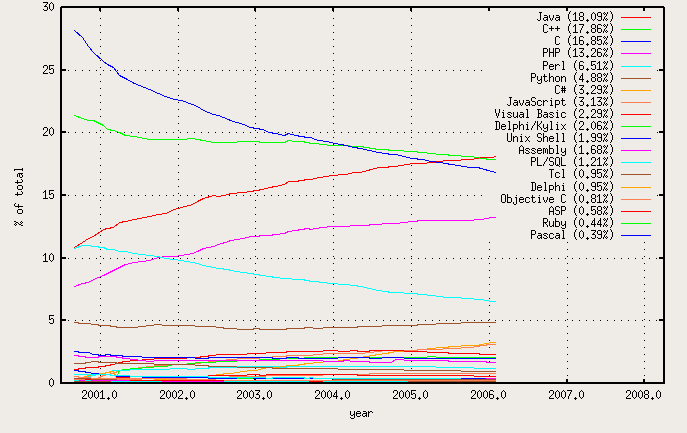
\includegraphics[width=\linewidth]{img/intro-language-sourceforge.png}%
        \rotatebox{90}{~~~\tiny\url{http://www.cs.berkeley.edu/}}
        \rotatebox{90}{~~~~~~~~\tiny\url{~flab/languages.html}}}
        
      \end{column}
    \end{columns}
\medskip
  \item \structure{Counting SLOC in Debian.}
    Quite different numbers...
    \end{itemize}

    \begin{columns}  
      \begin{column}{.35\linewidth}
        \setcounter{b}{0}
        \begin{tikzpicture}[scale=1.25]
          \foreach \p/\t/\c in {16/other/olive, 49/C/blue, 21/C++/green, 
            9/shell/yellow, 5/Java/red}
          {
            \setcounter{a}{\value{b}}
            \addtocounter{b}{\p}
            \drawSlice{\thea/100*360}{\theb/100*360}
            {\p\%}{\t}{\c}
          }        
        \end{tikzpicture}
      \end{column}
      \begin{column}{.5\linewidth}
        {\scriptsize More details:\\
        \url{http://debian-counting.libresoft.es/lenny/}\\
        See also: \url{http://www.dwheeler.com/sloc/}}

        \begin{itemize}
        \item Big codes are in C/C++ 
        \item Toy projects tend to be in Java
        \end{itemize}
        ~(but things change)
      \end{column}
    \end{columns}
\end{frame}
%%%%%%%%%%%%%%%%%%%%%%%%%%%%%%%%%%%%%%%%%%%%%%%%%%%%%%%%%%%%%%%%%%%%%
\begin{frame}{Why should we study the C language? Fast}
  \begin{itemize}
  \item \structure{C program typically execute faster than in other programs}
    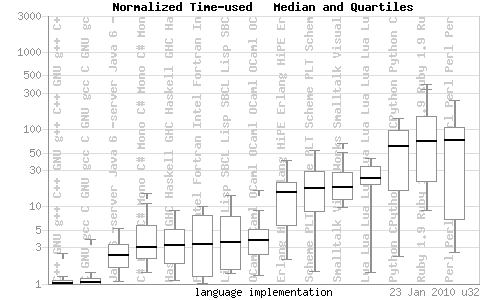
\includegraphics[width=.9\linewidth]{img/intro-shootout-fast.png}
    \rotatebox{90}{\tiny\url{http://shootout.alioth.debian.org/}}

  \item One could argue that this is because it has the best tools, but not
    only 
  \end{itemize}
\end{frame}
%%%%%%%%%%%%%%%%%%%%%%%%%%%%%%%%%%%%%%%%%%%%%%%%%%%%%%%%%%%%%%%%%%%%%
\begin{frame}{Studying the C language for educational purpose}
  \begin{block}{Understanding C helps you understanding the system as a whole}
    \begin{itemize}
    \item C is the closest high-level language to the machine
    \item Every OS are written in C, so lower interface is in C/C++ too
    \item \structure{OS/hardware co-evolution:} C conceptual model describes
      most hardware
    \end{itemize}
  \end{block}
  \begin{block}{Understanding C helps you writing better Java code}
    \begin{itemize}
    \item Java/.Net/Perl/etc hide underlying low-level mechanism
    \item But these mechanism can be very important (to performance for example)
    \item To understand how objects get passed by ref, realize that they are
      pointers
    \end{itemize}
  \end{block}
\end{frame}
%%%%%%%%%%%%%%%%%%%%%%%%%%%%%%%%%%%%%%%%%%%%%%%%%%%%%%%%%%%%%%%%%%%%%%%%%%%%%%%
\subsection{Why do we need to study C and UNIX together?}
\begin{frame}[squeeze]{Why do we need to study C and UNIX together?}
  \alert{\large Because they were invented together!}
  \vspace{-1.5\baselineskip}

    \begin{columns}
    \begin{column}{.55\linewidth}
      \includegraphics[width=\linewidth]{fig/intro-historique.fig}      
    \end{column}
    \begin{column}{.45\linewidth}
      \begin{block}{Unix history}        
        \begin{description}
        \item[1965] MULTICS: ambitious system project {\small(Bell Labs)}
        \item[1969] Bell Labs give up  \textsc{Multics}, 
          \textsc{Unics} begins 
        \item[1970] Unix: Official  Bell Labs project
        \item[1973] Rewrite in C\\
          Distribution to universities\\
          Sold by AT\&T
        \item[80-90] Unix War: {\small BSD vs. System V}\\
        \item[90-10] Normalization Effort (POSIX)
        \end{description}
      \end{block}\vspace{-\baselineskip}

      \begin{block}{C history}
        \begin{description}
        \item[1967] BCPL used at Bell Labs; 
        \item[1968] B [Thompson]: simplification
        \item[1971] C K\&R (somehow typed)
        \item[1983] C++: object oriented
        \item[1989] ANSI C; \structure{1990}: ISO C {\small(C90)}
        \item[1999] ISO C updated {\small(C99)}
        \end{description}
      \end{block}
    \end{column}
  \end{columns}
\end{frame}
%%%%%%%%%%%%%%%%%%%%%%%%%%%%%%%%%%%%%%%%%%%%%%%%%%%%%%%%%%%%%%%%%%%%%%%%%%%%%%%
\begin{frame}[squeeze]{What is Special About C?}
  \begin{block}{Low Level: sort of abstract assembly language of historical
      processors}
    \begin{itemize}
    \item Was invented on a PDP-11 with 24kb of memory: KISS!
      % The development of the C language, Dennis Ritchie.
    \item Process memory visible as an array of bytes
    \item Nothing in the language will prevent you from doing (really) stupid
      things
    \end{itemize}
    \textit{\small C combines the power of assembler with the portability of
      assembler.}

  \end{block}  
  \begin{block}{Extensible: most higher-level features doable in C}
    \begin{itemize}
    \item Self-modifying code, Introspection, Code migration, etc.
      (but all by yourself)
    \item (actually, JVM partially written in C/C++)
    \end{itemize}
    \textit{\small If you can't do it in ANSI C, it isn't worth doing.}
  \end{block}

  \begin{block}{Relatively Stable: almost backward compatible since seventies}
    \begin{itemize}
    \item Other languages got heavily lifted too often (but some heritages
      unpleasant)
    \end{itemize}
  \end{block}

  \begin{block}{C has hardly any runtime system}
    \begin{itemize}
    \item Small footprint, easily ported to new architectures 
      {\small (need to reinvent the wheel)}
    \end{itemize}
  \end{block}
\end{frame}
%%%%%%%%%%%%%%%%%%%%%%%%%%%%%%%%%%%%%%%%%%%%%%%%%%%%%%%%%%%%%%%%%%%%%%%%%%%%%%
\begin{frame}{So, should we use C once studied?}
  \begin{block}{Benefits}
    \begin{itemize}
    \item More control over the execution behaviour of programs
    \item More opportunity for performance tuning
    \item Access to low-level features of system
    \end{itemize}
  \end{block}\vspace{-.5\baselineskip}
  \begin{block}{Disadvantages}
    \begin{itemize}
    \item Need to do your own memory management
    \item Typically takes more lines of code to accomplish each task
    \item More opportunity to make mistakes
    \end{itemize}
  \end{block}\vspace{-.5\baselineskip}
  \begin{block}{Summary}
    \begin{itemize}
    \item C is a powerful programming tool for experts
    \item Presents many potential hazards for novices
    \item Helps you to understand low-level execution ideas
    \item Helps transforming you from a novice to an expert
    \item[$\leadsto$] Use it when you need it, avoid it when you don't need it
    \end{itemize}
  \end{block}  
\end{frame}
%%%%%%%%%%%%%%%%%%%%%%%%%%%%%%%%%%%%%%%%%%%%%%%%%%%%%%%%%%%%%%%%%%%%%%%%%%%%%
\section{C as Second Language}\sectionpage
\subsection{C vs. Java}
\begin{frame}{C as Second Language}
  \begin{block}{Similarities between C and Java}
    \begin{itemize}
    \item \structure{Operators}
      \begin{itemize}
      \item \structure{Arithmetic} (+,-,*,/,\% ;  ++,- -,*=,\ldots);
        \structure{Bitwise} (\&,$|$,\^{},!,$<<$,$>>$)
      \item \structure{Relational} ($<$,$>$,$<$=,$>$=,==,!=);
      \structure{Logical} \&\&, $||$, !, (a?b:c)
      \end{itemize}
    \item \structure{Keywords and Language Constructs}\vspace{-.5\baselineskip}
      \begin{columns}
        \begin{column}{.5\linewidth}
          \begin{itemize}
          \item \texttt{if( )\{ \} else \{ \}}
          \item \texttt{while( )\{ \}}
          \item \texttt{switch( ) \{ case 0: ... \}}
          \end{itemize}
        \end{column}
        \begin{column}{.45\linewidth}
          \begin{itemize}
          \item \texttt{for(i=0; i<100; i++)\{ \}}
          \item \texttt{do \{ \} while( )}
          \item \texttt{break}, \texttt{continue}, \texttt{return}
          \end{itemize}
        \end{column}
      \end{columns}\smallskip
    \item \structure{Basic (primitive) types:} void, int, short, long; float,
      double; char.\\ {\small No boolean, use int instead  (0=False; anything
        else=True)}

    \item \structure{Function declarations:} \texttt{\small int fact(int a)\{return a==0 ? 1 : a*fact(a-1);\}}
    \end{itemize}
  \end{block}\vspace{-\baselineskip}

  \begin{block}{Differences between C and Java}
    \begin{itemize}
    \item \structure{No exception:} usually rely on int error code instead 
      {\small(and usually a pain)}
    \item \structure{No class/package/interface:} code modularity different
      {\small(not compiler-enforced)}
    \item \structure{No garbage collector:} alloc and free manually needed
      memory {\small(incredible pain)}
    \end{itemize}
  \end{block}
\end{frame}
%%%%%%%%%%%%%%%%%%%%%%%%%%%%%%%%%%%%%%%%%%%%%%%%%%%%%%%%%%%%%%%%%%%%%%%%%%
\begin{frame}[squeeze]{C as Second Language}
  \begin{block}{C seems familiar when you know Java}
    \begin{itemize}
    \item Actually, that's Java which is highly inspired from C/C++
    \item Feels like a Java without any object but with full access to
      everything 
    \end{itemize}
  \end{block}

  \begin{block}{C is like Java without comfort and without any protections}
    \begin{itemize}
    \item Standard library is poor (but huge amount of extensions)
    \item Compiler is incredibly permissive (by default)
    \item It's possible to shoot yourself in the foot in Java, that's common in
      C
    \item On error, Java displays a stack trace, C spits ``segfault'' or
      ``invalid free'' errors
    \end{itemize}
  \end{block}
  
  \begin{boitequote}{Doug Gwyn}
    Unix was not designed to stop people from doing stupid things, because
    that would also stop them from doing clever things.
  \end{boitequote}
  \begin{block}{C main specificities in a Nutshell}
    \begin{itemize}
    \item Memory fully accessible through \textit{pointers}
    \item Arrays are handled as pointer to memory
    \item Declaration syntax very similar to usage syntax (to the price of
      readability)
    \end{itemize}
  \end{block}
\end{frame}
%%%%%%%%%%%%%%%%%%%%%%%%%%%%%%%%%%%%%%%%%%%%%%%%%%%%%%%%%%%%%%%%%%%%%%%%%%%%
\subsection{How to survive in C?}
\begin{frame}{How to survive in C?}
  \begin{block}{Use the tools that can help you}
    \begin{itemize}
    \item Use the \structure{compiler warning flags} \texttt{-Wall} mandatory,
      other usefull
    \item Use a \structure{proper editor} (able of colorization, auto-indent,
      compile easily)
      \begin{itemize}
      \item \structure{Good editors:} emacs \& vi (historical),
        Eclipse{\small/CDT} (my personal favorite)
      \item \structure{Bad editor:} gedit (not good for text, BAD for code)
      \end{itemize}
    \item The \structure{debugger} (\texttt{gdb}) must become your friend
      quickly
    \item \structure{valgrind} is a piece of magic (C coding without it is
      masochism)
    \end{itemize}
  \end{block}

  \begin{block}{Don't assume you're a genius (ie, don't do stupid things ---
      yet)}
    \begin{itemize}
    \item Pay attention to the modularity of your code (not compiler-enforced anyhow)
    \item Document your code (with readable comments, or doxygen for bigger
      projects) 
    \item Get some discipline (coding convention), and stick to it
      \begin{itemize}
      \item Symbol naming (my\_variable or myVariable), indentation, etc.
      \item Which one is not very important. Pick one, and stick to it
      \end{itemize}
    \item Keep it simple: it's easy to write unreadable C code
    \end{itemize}
  \end{block}
\end{frame}
%%%%%%%%%%%%%%%%%%%%%%%%%%%%%%%%%%%%%%%%%%%%%%%%%%%%%%%%%%%%%%%%%%%%%%%%%%%%%
\begin{frame}[fragile]{Bad Style Coding as a Game}
  \begin{block}{The International Obfuscated C Code Contest
      (\url{www.ioccc.org})} 
    \begin{itemize}
    \item Yearly contest of intentionally obfuscated codes 
      {\small(in C; exist for other languages)}
    \end{itemize}
  \end{block}\vspace{-.4\baselineskip}
  \begin{block}{Example: \visible<2->{Full (interactive) Maze Escape Game}
      {\normalsize (arachnid, 2004 entry)}}\vspace{-.8\baselineskip}
    \begin{columns}
      \begin{column}{.6\linewidth}
    \vbox{\begin{Verbatim}[fontsize=\tiny]
#include <ncurses.h>/*****************************************************/
            int               m[256                   ] [         256   ],a
 ,b   ;;;   ;;;   WINDOW*w;   char*l=""   "\176qxl"   "q"   "q"   "k"   "w\
xm"   "x"   "t"         "j"         "v"         "u"         "n"         ,Q[
 ]=   "Z"   "pt!ftd`"   "qdc!`eu"   "dq!$c!nnwf"/**   ***   */"t\040\t";c(
int   u ,         int         v){                     v?m   [u]         [v-
 1]   |=2,m[u][v-1] &   48?W][v-1   ] &   15]]):0:0;u?m[u   -1][v]|=1   ,m[
 u-               1][   v]&         48?               W-1   ][v         ]&
15]   ]):0:0;v<   255   ?m[   u][v+1]|=8,m[u][v+1]&   48?   W][   v+1]&15]]
):0         :0;         u <               255   ?m[   u+1         ][v   ]|=
4,m[u+1][   v]&48?W+1][v]&15]]):0:0;W][   v]&   15]   ]);}cu(char*q){   return
 *q               ?cu   (q+         1)&         1?q   [0]               ++:
q[0   ]--   :1;   }d(   int   u ,   int/**/v,   int/**/x,   int   y){   int
Y=y   -v,   X=x         -u;   int         S,s   ;Y<         0?Y   =-Y   ,s,
s=-   1:(   s=1);X<0?X=-X,S   =-1  :(S=   1);   Y<<=   1;X<<=1;   if(X>Y){
int   f=Y               -(X   >>1   );;               while(u!=         x){
f>=   0?v+=s,f-=X:0;u   +=S   ;f+=   Y;m[u][v]|=32;mvwaddch(w,v   ,u,   m[u
 ][               v]&   64?   60:         46)         ;if         (m[   u][
v]&16){c(u,v);;   ;;;   ;;;   return;}}   }else{int   f=X   -(Y>>1);;   while
 (v   !=y         ){f   >=0         ?u   +=S,               f-=         Y:0
 ;v   +=s   ;f+=X;m[u][v]|=   32;mvwaddch(w,v   ,u,m[u][v]&64?60:46);if(m[u
 ][                     v]&         16)   {c(   u,v                     );
  ;   return;;;}}}}Z(   int/**/a,   int   b){   }e(   int/**/y,int/**/  x){
int               i ;         for         (i=         a;i               <=a
+S;i++)d(y,x,i,b),d(y,x,i,b+L);for(i=b;i<=b+L;i++)d(y,x,a,i),d(y,x,a+   S,i
 );                     ;;;         ;;;         ;;;               ;;;   ;
  mvwaddch(w,x,y,64);   ;;;   ;;;   ;;;   prefresh(   w,b,a,0,0   ,L-   1,S-1
);}             main(         int               V ,   char              *C[
  ]   ){FILE*f=   fopen(V==1?"arachnid.c"/**/   :C[   1],"r");int/**/x,y,c,
                 (source code cut here)
    \end{Verbatim}
  }%$
      \end{column}
      \begin{column}{.4\linewidth}%~\medskip
        \visible<3->{
          \begin{block}{Screenshoot}\medskip
            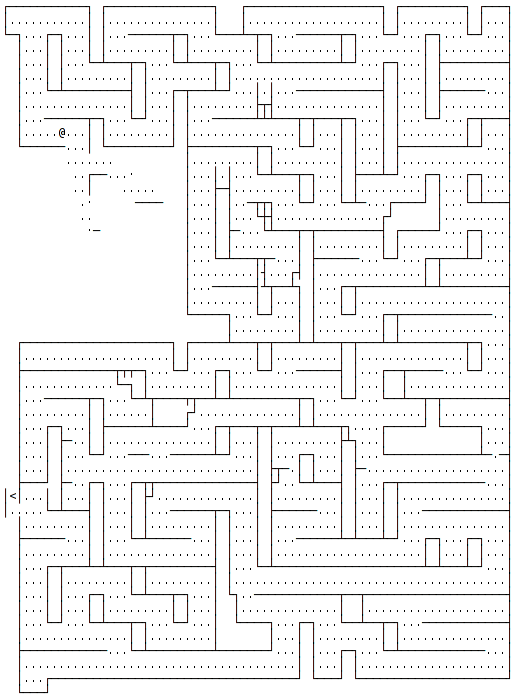
\includegraphics[width=\linewidth]{img/maze.png}          
          \end{block}
        }
      \end{column}
    \end{columns}

  \end{block}
\end{frame}
%%%%%%%%%%%%%%%%%%%%%%%%%%%%%%%%%%%%%%%%%%%%%%%%%%%%%%%%%%%%%%%%%
\begin{frame}[fragile]{Recreational Obfuscation: Phillips entry of IOCCC'88}
  \begin{Verbatim}[fontsize=\footnotesize,frame=single,label=Program code]
#include <stdio.h>
main(t,_,a)char *a;{return!0<t?t<3?main(-79,-13,a+main(-87,1-_,
main(-86,0,a+1)+a)):1,t<_?main(t+1,_,a):3,main(-94,-27+t,a)&&t==2?_<13?
main(2,_+1,"%s %d %d\n"):9:16:t<0?t<-72?main(_,t,
"@n'+,#'/*{}w+/w#cdnr/+,{}r/*de}+,/*{*+,/w{%+,/w#q#n+,/#{l,+,/n{n+,/+#n+,/#\
;#q#n+,/+k#;*+,/'r :'d*'3,}{w+K w'K:'+}e#';dq#'l \
q#'+d'K#!/+k#;q#'r}eKK#}w'r}eKK{nl]'/#;#q#n'){)#}w'){){nl]'/+#n';d}rw' i;# \
){nl]!/n{n#'; r{#w'r nc{nl]'/#{l,+'K {rw' iK{;[{nl]'/w#q#n'wk nw' \
iwk{KK{nl]!/w{%'l##w#' i; :{nl]'/*{q#'ld;r'}{nlwb!/*de}'c \
;;{nl'-{}rw]'/+,}##'*}#nc,',#nw]'/+kd'+e}+;#'rdq#w! nr'/ ') }+}{rl#'{n' ')# \
}'+}##(!!/")
:t<-50?_==*a?putchar(31[a]):main(-65,_,a+1):main((*a=='/')+t,_,a+1)
  :0<t?main(2,2,"%s"):*a=='/'||main(0,main(-61,*a,
"!ek;dc i@bK'(q)-[w]*%n+r3#l,{}:\nuwloca-O;m .vpbks,fxntdCeghiry"),a+1);}
  \end{Verbatim}    
  \begin{minipage}{.5\linewidth}
  \begin{Verbatim}[fontsize=\tiny,frame=single,label=Output]
On the first day of Christmas my true love gave to me
a partridge in a pear tree.

On the second day of Christmas my true love gave to me
two turtle doves
and a partridge in a pear tree.

On the third day of Christmas my true love gave to me
three french hens, two turtle doves
and a partridge in a pear tree.

On the fourth day of Christmas my true love gave to me
four calling birds, three french hens, two turtle doves
and a partridge in a pear tree.

On the fifth day of Christmas my true love gave to me
five gold rings;
four calling birds, three french hens, two turtle doves
and a partridge in a pear tree.

On the sixth day of Christmas my true love gave to me
six geese a-laying, five gold rings;
four calling birds, three french hens, two turtle doves
and a partridge in a pear tree.

On the seventh day of Christmas my true love gave to me
seven swans a-swimming,
six geese a-laying, five gold rings;
four calling birds, three french hens, two turtle doves
and a partridge in a pear tree.

  \end{Verbatim}    
  \end{minipage}~\begin{minipage}{.5\linewidth}
  \begin{Verbatim}[fontsize=\tiny,frame=single,label=Output (cont)]
On the eighth day of Christmas my true love gave to me
eight maids a-milking, seven swans a-swimming,
six geese a-laying, five gold rings;
four calling birds, three french hens, two turtle doves
and a partridge in a pear tree.

On the ninth day of Christmas my true love gave to me
nine ladies dancing, eight maids a-milking, seven swans a-swimming,
six geese a-laying, five gold rings;
four calling birds, three french hens, two turtle doves
and a partridge in a pear tree.

On the tenth day of Christmas my true love gave to me
ten lords a-leaping,
nine ladies dancing, eight maids a-milking, seven swans a-swimming,
six geese a-laying, five gold rings;
four calling birds, three french hens, two turtle doves
and a partridge in a pear tree.

On the eleventh day of Christmas my true love gave to me
eleven pipers piping, ten lords a-leaping,
nine ladies dancing, eight maids a-milking, seven swans a-swimming,
six geese a-laying, five gold rings;
four calling birds, three french hens, two turtle doves
and a partridge in a pear tree.

On the twelfth day of Christmas my true love gave to me
twelve drummers drumming, eleven pipers piping, ten lords a-leaping,
nine ladies dancing, eight maids a-milking, seven swans a-swimming,
six geese a-laying, five gold rings;
four calling birds, three french hens, two turtle doves
and a partridge in a pear tree.
  \end{Verbatim}
\end{minipage}
\end{frame}
%%%%%%%%%%%%%%%%%%%%%%%%%%%%%%%%%%%%%%%%%%%%%%%%%%%%%%%%%%%%%%%%%%%%%%%
%%
%% Pas possible de faire apparaitre des Verbatim en animation
%%   => dupplication du source (irk!)
%%
\begin{frame}<handout:0>[fragile,t]{Bad Style Coding as an Art}
  \begin{block}{Another example\visible<2->{: Computing Integer Square Roots}}
    \medskip
    \begin{columns}
      \begin{column}{.3\linewidth}        
    \begin{Verbatim}[fontsize=\scriptsize]
#include <stdio.h>
int l;int main(int o,char **O,
int I){char c,*D=O[1];if(o>0){
for(l=0;D[l              ];D[l
++]-=10){D   [l++]-=120;D[l]-=
110;while   (!main(0,O,l))D[l]
+=   20;   putchar((D[l]+1032)
/20   )   ;}putchar(10);}else{
c=o+     (D[I]+82)%10-(I>l/2)*
(D[I-l+I]+72)/10-9;D[I]+=I<0?0
:!(o=main(c/10,O,I-1))*((c+999
)%10-(D[I]+92)%10);}return o;}     
    \end{Verbatim}
      \end{column}
      \begin{column}{.32\linewidth}        
        \visible<2->{\structure{It actually works}\\
        \fbox{\vbox{\scriptsize\texttt{\noindent
\$ ./cheong 1234\\
35}}}\\
{\scriptsize($35\times 35=1225$; $35\times 36=1296$)}\\
\medskip\fbox{\vbox{\scriptsize\texttt{\noindent
\$ ./cheong 112233445566\\
335012}}}\\
{\scriptsize$335012\times 335012=112233040144$
$335013\times 335013=112233710169$
}}
      \end{column}
      \begin{column}{.25\linewidth}
      \end{column}
    \end{columns}
  \end{block}

\end{frame}
\begin{frame}[fragile,t]{Bad Style Coding as an Art}
  \begin{block}{Another example: Computing Interger Square Roots}
    \medskip
    \begin{columns}
      \begin{column}{.3\linewidth}        
    \begin{Verbatim}[fontsize=\scriptsize]
#include <stdio.h>
int l;int main(int o,char **O,
int I){char c,*D=O[1];if(o>0){
for(l=0;D[l              ];D[l
++]-=10){D   [l++]-=120;D[l]-=
110;while   (!main(0,O,l))D[l]
+=   20;   putchar((D[l]+1032)
/20   )   ;}putchar(10);}else{
c=o+     (D[I]+82)%10-(I>l/2)*
(D[I-l+I]+72)/10-9;D[I]+=I<0?0
:!(o=main(c/10,O,I-1))*((c+999
)%10-(D[I]+92)%10);}return o;}     
    \end{Verbatim}
      \end{column}
      \begin{column}{.32\linewidth}        
        \structure{It actually works}\\
        \fbox{\vbox{\scriptsize\texttt{\noindent
\$ ./cheong 1234\\
35}}}\\
{\scriptsize($35\times 35=1225$; $35\times 36=1296$)}\\
\medskip\fbox{\vbox{\scriptsize\texttt{\noindent
\$ ./cheong 112233445566\\
335012}}}\\
{\scriptsize$335012\times 335012=112233040144$
$335013\times 335013=112233710169$
}
      \end{column}
      \begin{column}{.25\linewidth}
        \structure{Author claim: code self-documented$\ldots$}

        \begin{Verbatim}[fontsize=\tiny]
#include <stdio.h>
int l;int main(int o,char **O,
int I){char c,*D=O[1];if(o>0){
for(l=0;D[l              ];D[l
++]-=10){D   [l++]-=120;D[l]-=
110;while   (!main(0,O,l))D[l]
+=   20;   putchar((D[l]+1032)
/20   )   ;}putchar(10);}else{
c=o+     (D[I]+82)%10-(I>l/2)*
(D[I-l+I]+72)/10-9;D[I]+=I<0?0
:!(o=main(c/10,O,I-1))*((c+999
)%10-(D[I]+92)%10);}return o;}               
        \end{Verbatim}
      \end{column}
    \end{columns}
  \end{block}

  \visible<2->{
  \begin{boitequote}{William Strunk, Jr. (1918)}
    It is an old observation that the best writers sometimes disregard the
    rules of rhetoric.  When they do so, however, the reader will usually find
    in the sentence some compensating merit, attained at the cost of the
    violation. \textbf{Unless he is certain of doing as well, he will probably
      do best to follow the rules}.
  \end{boitequote}}
\end{frame}
%%%%%%%%%%%%%%%%%%%%%%%%%%%%%%%%%%%%%%%%%%%%%%%%%%%%%%%%%%%%%%%%%%%%%%%%%%%%
\begin{frameTODO}{Bad Style Coding for Efficiency}
  Parler ici du duff device. Mais ils sont encore un peu frais pour parler
  d'horreurs pareilles. Ca leur fera meme pas peur je pense.
http://en.wikipedia.org/wiki/Duff%27s_device
\end{frameTODO}
%%%%%%%%%%%%%%%%%%%%%%%%%%%%%%%%%%%%%%%%%%%%%%%%%%%%%%%%%%%%%%%%%%%%%%%%%%%%
\begin{frame}[t]{Last one, just for fun: dhyang IOCCC'00}

  \vspace{-.5\baselineskip} Saitou Hajime image \visible<2->{that prints a
    prog} \visible<3->{that prints a prog} \visible<4->{that prints a prog}
  \visible<5->{\ldots}

  \visible<5->{Repeating endlessly "aku soku zan", Hajime's motto meaning
    \textit{slay evil imediatly}.}\medskip

  \begin{columns}
    \begin{column}{.25\linewidth}\vspace{-\baselineskip}
      \begin{block}{Source code}\medskip
        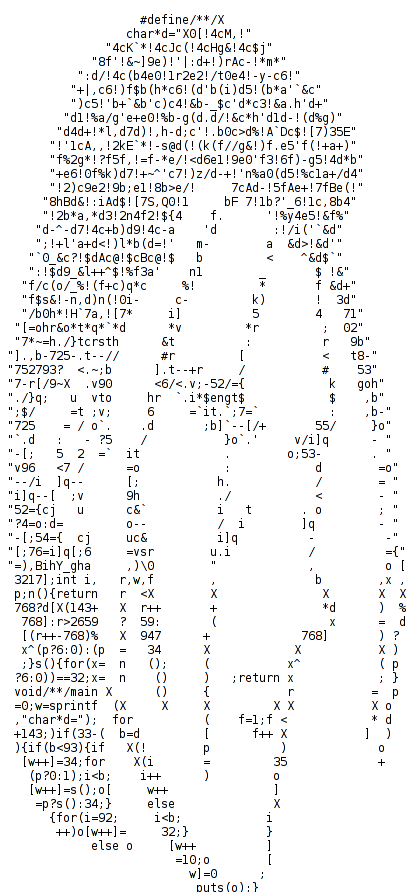
\includegraphics[width=\linewidth]{img/dhyang1.png}        
      \end{block}
    \end{column}

    \begin{column}{.3\linewidth}\vspace{-\baselineskip}
      \begin{block}<2->{Output 1}\medskip
        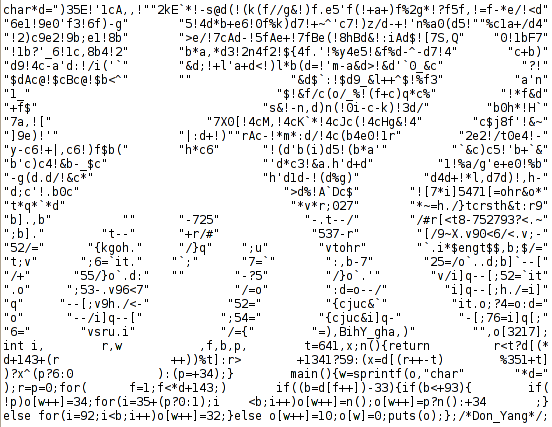
\includegraphics[width=\linewidth]{img/dhyang2.png}        
      \end{block}
      \begin{block}<4->{Output 3}\medskip
        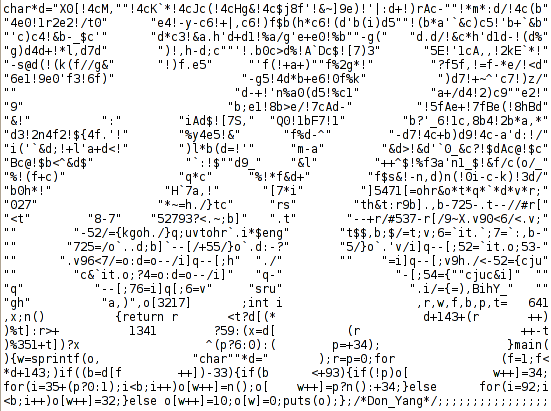
\includegraphics[width=\linewidth]{img/dhyang4.png}        
      \end{block}
    \end{column}

    \begin{column}{.3\linewidth}\vspace{-\baselineskip}
      \begin{block}<3->{Output 2}\medskip
        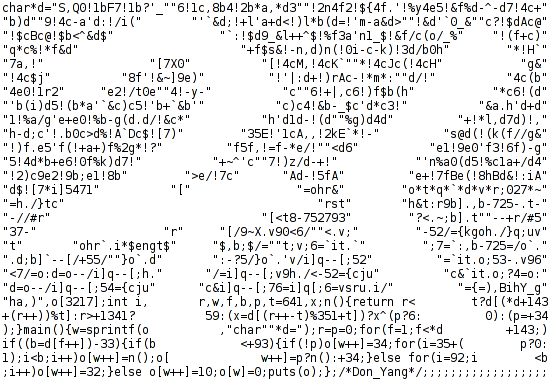
\includegraphics[width=\linewidth]{img/dhyang3.png}        
      \end{block}
      \begin{block}<5->{Output 4 (=1)}\medskip
        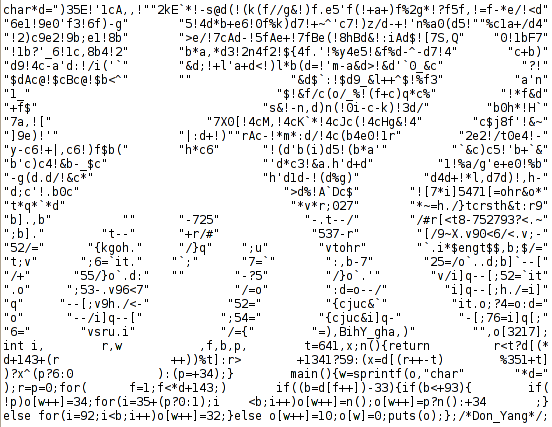
\includegraphics[width=\linewidth]{img/dhyang2.png}        
      \end{block}
    \end{column}      
  \end{columns}
\end{frame}
%%%%%%%%%%%%%%%%%%%%%%%%%%%%%%%%%%%%%%%%%%%%%%%%%%%%%%%%%%%%%%%%%%%%%%%%%%%
\subsection{Your first C program}
\begin{frame}[fragile]{Your first C program}

  \begin{columns}
    \begin{column}{.47\linewidth}
      \begin{block}{The classical Hello World}\medskip
       \begin{Verbatim}[gobble=9,frame=single,fontsize=\small,label=hello.c,numbers=left]
         #include <stdio.h>
         int main(int argc, char *argv[]){
           printf("Hello, world\n");
         }
       \end{Verbatim}
      \end{block}  

      \begin{block}{Compile and run it}
        \begin{Verbatim}[gobble=9,fontsize=\small,frame=single,numbers=left]
          $ gcc -Wall hello.c -o hello
          $ ./hello
        \end{Verbatim}
      \end{block}
    \end{column}

    \begin{column}{.53\linewidth}
      \begin{block}{For the record: same in Java}\medskip
       \begin{Verbatim}[gobble=9,fontsize=\small,frame=single,label=hello.c]
         class HelloWorld {
          public static void main(String[]arg){
           System.out.println("Hello, world");
         }}
       \end{Verbatim}        
      \end{block}
      \begin{block}{Compiling and running Java code}
        \begin{Verbatim}[gobble=9,fontsize=\small,frame=single]
          $ javac HelloWorld.java
          $ java -cp . HelloWorld
        \end{Verbatim}
      \end{block}
    \end{column}
  \end{columns}
  \begin{block}{Explanations}
    \begin{itemize}
    \item \texttt{\#include} can be seen as the equivalent of \texttt{import}
      directives
    \item \texttt{main} is the \textit{entry point} of every program (same in C
      and Java)
    \end{itemize}
  \end{block}
\end{frame}
%%%%%%%%%%%%%%%%%%%%%%%%%%%%%%%%%%%%%%%%%%%%%%%%%%%%%%%%%%%%%%%%%%%%%%%%%%%%%%
\begin{frame}{C Compilation Process}
  \begin{block}{Compiling a C program involves 3 separate tools}
    \begin{enumerate}
    \item \structure{Pre-processor:} Rewrites the code according to the defined
      \textit{\alert{macros}}
      \begin{itemize}
      \item Lines begining with "\#" are macros
      \item \texttt{\#define name value}: declare a sort of automatic
        search/replace
      \item \texttt{\#define name(params) value}: search/replace but with
        arguments
      \item \texttt{\#include "file"}: inline the content of the given file
      \item \texttt{\#ifdef name}/\texttt{\#else}/\texttt{\#endif}: mask parts
        of the file if \texttt{name} is defined
      \end{itemize}
    \item \structure{Compiler:} Translates the code into assembly
    \item \structure{Linker:} Take elements in assembly and resolve library
      dependencies
      \begin{itemize}
      \item If your code uses function \texttt{cos()}, you need the math lib
      \item The linker solves a puzzle to ensure that every used function get
        defined 
      \end{itemize}
    \end{enumerate}
  \end{block}

  \begin{block}{This process is rather transparent to the user}
    \begin{itemize}
    \item You edit your code (in emacs/vi/eclipse)
    \item You launch gcc, which lauches mandatory tools automatically
    \item You mainly need to know that when you get error messages
    \end{itemize}
  \end{block}
\end{frame}
%%%%%%%%%%%%%%%%%%%%%%%%%%%%%%%%%%%%%%%%%%%%%%%%%%%%%%%%%%%%%%%%%%%%%%%%%%%%
\begin{frame}[squeeze]{What if you get error messages when compiling}
  \vspace{-.3\baselineskip}
  \begin{block}{Some examples}
    \begin{itemize}\vspace{-.3\baselineskip}
    \item \texttt{\small foo.c:71:2: error: invalid preprocessing directive
        \#deifne}\\
      \structure{The preprocessor is not happy: check file \texttt{foo.c}, line
        71, column 2}
      
    \item \texttt{\small foo.c:72: error: expected ')' before `char'}\\
      \structure{Compiler's not happy (syntax error)}
    \item \texttt{\small foo.c:74: error: redefinition of 'myFunc'\\
        foo.c:72: error: previous definition of 'myFunc' was here}\\
      \structure{Defining the same function twice makes the linker unhappy}
    \item \texttt{/usr/lib/crt1.o: In function `\_start':\\
        (.text+0x18): undefined reference to `main'\\
        collect2: ld returned 1 exit status}\\
      \structure{A function is used, but never defined} \\
      {\small(see RS lecture next year to understand the detail of the message)}
    \item \texttt{Segmentation fault ./myProg}\\
      \structure{Your program messed up the memory (valgrind knows where)}
    \end{itemize}
  \end{block}\vspace{-.8\baselineskip}

  \begin{block}{How to react when you get error messages (and you will)}
    \begin{itemize}\vspace{-.3\baselineskip}
    \item \alert{Don't panic}, even if the message seem cryptic (they often are)
    \item \alert{Read the message:} they are sometimes even understandable
    \item \alert{Don't even read the \textbf{second} message:} the parser often
      gets lost after first error
    \end{itemize}
  \end{block}
\end{frame}
%%%%%%%%%%%%%%%%%%%%%%%%%%%%%%%%%%%%%%%%%%%%%%%%%%%%%%%%%%%%%%%%%%%%%%%%%%%%%%
\begin{frame}{Conclusion on C (for now)}
  \begin{block}{C is the modern assembly language}
    \begin{itemize}
    \item It's quite prehistorical
      \begin{itemize}
      \item Compilation process not trivial (even with only one file)
      \item Cryptic error messages
      \item No fancy stuff in standard library
      \end{itemize}
    \item Programs can be really fast
      \begin{itemize}
      \item If you do them right; easy to code slow C programs too
      \end{itemize}
    \item You have the full power of doing everything
      \begin{itemize}
      \item No matter what you want to code, it's possible in C
      \item A lot of code were already developed in C (check \url{koders.com})
      \item C poses no rule to limit your imagination\ldots
      \item \ldots but there is no barrier to prevent you doing stupid things
      \end{itemize}
    \end{itemize}
  \end{block}
  \begin{block}{You need to master C to understand your machine}
    \begin{itemize}
    \item The operating system is in C, just like the virtual machines
    \item And then, you're free to use it or not\\
      Depending on whether you're seeking for fast programs or fast coding
    \end{itemize}
  \end{block}
\end{frame}
%%%%%%%%%%%%%%%%%%%%%%%%%%%%%%%%%%%%%%%%%%%%%%%%%%%%%%%%%%%%%%%%%%%%%%%%%%%%%
\section{First steps in Unix}\sectionpage
\begin{frame}[squeeze]{First steps in Unix}
  \begin{block}{This OS gives a central role to \textbf{files}}
    \begin{itemize}
    \item Contains data and executable programs (quite usual)
      \medskip
    \item \structure{Communication with user} : config files,
      \texttt{stdin}, \texttt{stdout}
    \item \structure{Communication between processes}: sockets, pipes, etc.
      \medskip
    \item \structure{Interface to the kernel}: \texttt{/proc}
    \item \structure{Interface to the hardware}: peripheral in \texttt{/dev}
    \end{itemize}
  \end{block}

  \begin{block}<2->{The \textbf{Terminal} is an interface of choice}
    \begin{itemize}
    \item Graphical interfaces exist too, but I still prefer the terminal
    \item Lots of tricks make you more efficient with the terminal\\
      (more button on my keyboard than on my mouse)
    \item If you can't do it in one step, type a one-line script directly
    \end{itemize}
  \end{block}

  \begin{block}<3->{Read The Fine Manual (RTFM)}
    \begin{itemize}
    \item The command \texttt{man} gives you access to a large corpus of
      knowledge
    \item \texttt{man prog} or \texttt{man function} $\leadsto$
      documentation of that program or function
    \end{itemize}
  \end{block}
\end{frame}
%%%%%%%%%%%%%%%%%%%%%%%%%%%%%%%%%%%%%%%%%%%%%%%%%%%%%%%%%%%%%%%%%%%%%%%%%% 
\subsection{Désignation des fichiers}
\begin{frame}<trans:0>\frametitle{Désignation des fichiers}


  \begin{block}{Désignation symbolique (nommage): \alert{Organisation
        hiérarchique}}
    
    \begin{itemize}
    \item \structure{Noeuds intermédiaires:} répertoires
      (\textit{directory} -- ce sont aussi des fichiers)
    \item \structure{Noeuds terminaux:} fichiers simples
    \item \structure{Nom absolu d'un fichier:} le chemin d'accès depuis la
      racine

    \end{itemize}
  \end{block}

  \begin{columns}
    \begin{column}{.45\textwidth}
      \begin{block}{Exemples de chemins absolus :}
        \texttt{\footnotesize
          \begin{itemize}
          \item[] /
          \item[] /bin
          \item[] /usr/local/bin/prog
          \item[] /home/bob/conf/main.tex
          \item[] /home/jim/code/main.c
          \end{itemize}      
        }  
      \end{block}     
    \end{column}

    \begin{column}{.45\textwidth}
      \includegraphics{fig/io-sgf.fig}
    \end{column}
  \end{columns}
\end{frame}

%%%%%%%%%%%%%%%%%%%%%%%%%%%%%%%%%%%%%%%%%%%%%%%%%%%%%%%%%%%%%%%%%%%%%%%%%% 

\begin{frame}<trans:0>\frametitle{Raccourcis pour simplifier la
    désignation}

  \begin{block}{Noms relatifs au répertoire courant}
    \begin{itemize}
    \item Depuis \texttt{/home/bob},~~ \texttt{conf/main.tex} =
      \texttt{/home/bob/conf/main.tex}
    \end{itemize}
  \end{block}

  \begin{block}{Abréviations}
    \begin{itemize}
    \item \structure{Répertoire père}: depuis \texttt{/home/bob},
      \texttt{\texttt{\alert{..}}/jim/code} = \texttt{/home/jim/code}
    \item \structure{Répertoire courant}: depuis \texttt{/bin},
      \texttt{\texttt{\alert{.}}/prog1} = \texttt{/bin/prog1}
    \item Depuis n'importe où, \texttt{\alert{$\sim$}}bob/ = /home/bob/ et \alert{$\sim$}/ = /home/$<$moi$>$/
    \end{itemize} 
  \end{block}

  \begin{columns}
    \begin{column}{.68\textwidth}
      \begin{block}{Liens symboliques}
        Depuis \texttt{/home/jim}
        \begin{itemize}
        \item Création du lien: \texttt{ln -s} \textit{cible nom\_du\_lien}\\
          Exemple: \texttt{ln -s /bin/prog1 monprog}
        \item \texttt{/home/jim/prog1} désigne \texttt{/bin/prog1}
        \item Si la cible est supprimée, le lien devient invalide
        \end{itemize}
      \end{block}
    \end{column}    
    \begin{column}{.3\textwidth}
      \includegraphics{fig/io-lien.fig}
    \end{column}
  \end{columns}
\end{frame}
%%%%%%%%%%%%%%%%%%%%%%%%%%%%%%%%%%%%%%%%%%%%%%%%%%%%%%%%%%%%%%%%%%%%%%%%%% 
\begin{frame}\frametitle{Règles de recherche des exécutables}
    \begin{itemize}
    \item Taper le chemin complet des exécutable (/usr/bin/ls) est lourd
    \item $\Rightarrow$ on tape le nom sans le chemin et le shell cherche
    \item Variable environnement PATH: liste de répertoires à examiner
      successivement\\
      {\footnotesize \url{/usr/local/bin:/usr/local/sbin:/sbin:/usr/sbin:/bin:/usr/bin:/usr/bin/X11}}

    \item Commande \texttt{which} indique quelle version est utilisée
    \end{itemize}

    \begin{exo}{Comment exécuter un script nommé \texttt{gcc} dans le répertoire
        courant?}
      \begin{itemize}
      \item \structure{Solution 1}: \reponse{export PATH=".:\$PATH"; gcc $<$bla$>$}
      \item \structure{Solution 2}: \reponse{./gcc $<$bla$>$}
      \end{itemize}
    \end{exo}
\end{frame}
%%%%%%%%%%%%%%%%%%%%%%%%%%%%%%%%%%%%%%%%%%%%%%%%%%%%%%%%%%%%%%%%%%%%%%%%%% 
\begin{frame}<trans:0>\frametitle{Utilisations courantes des fichiers}

  \begin{itemize}
  \item Unix: fichiers = suite d'octets sans structure interprétée par
    utilisateur
  \item Windows: différencie fichiers textes (où $\backslash$n est modifié)
    des fichiers binaires
  \end{itemize}

  \begin{block}{Programmes exécutables}
    \begin{itemize}
    \item Commandes du système ou programmes créés par un utilisateur
    \item \structure{Exemple}: \texttt{gcc -o test test.c ; ./test} \\
      \trou{Produit programme exécutable dans fichier \texttt{test}; exécute
      le programme test}
    \item \structure{Question}: pourquoi
      \underline{\textbf{./}}\texttt{test} ?
      \reponse{(car test est un binaire classique: \texttt{\tiny if test \$n -le 0;})}
    \end{itemize}
  \end{block}\vspace{-\baselineskip}

  \begin{block}{Fichiers de données}
    \begin{itemize}
    \item Documents, images, programmes sources, etc.
    \item \structure{Convention:} \trou{le suffixe indique la nature du contenu}\\
      \structure{Exemples} : .c (programme C), .o (binaire translatable,
      cf. plus loin), .h (entête C), .gif (un format d'images), .pdf
      (Portable Document Format), \textit{etc.}\\
      \structure{Remarque:} ne pas faire une confiance aveugle à
      l'extension (\textit{cf.}~ \texttt{man file})
    \end{itemize}
  \end{block}\vspace{-\baselineskip}
  
  \begin{block}{Fichiers temporaires servant pour la communication}
    \begin{itemize}
    \item Ne pas oublier de les supprimer après usage
    \item On peut aussi utiliser des tubes (\textit{cf.} RS l'an prochain)
    \end{itemize}
  \end{block}
\end{frame}
%%%%%%%%%%%%%%%%%%%%%%%%%%%%%%%%%%%%%%%%%%%%%%%%%%%%%%%%%%%%%%%%%%%%%%%%%%%%%
\subsection{Protection des fichiers}
\begin{frame}<trans:0>\frametitle{Protection des fichiers: généralités}
  \begin{block}{Définition (générale) de la sécurité}
    \begin{itemize}
    \item \structure{confidentialité} : \trou{informations accessibles aux seuls
      usagers autorisés}\vspace{-.5\baselineskip}
    \item \structure{intégrité} : \trou{pas de modifications indésirées}
      \vspace{-.5\baselineskip}
    \item \structure{contrôle d'accès} : \trou{qui a le droit de faire
        quoi} \vspace{-.5\baselineskip}
    \item \structure{authentification} : \trou{garantie qu'un usager est
        bien celui qu'il prétend être}
    \end{itemize}
  \end{block}\vspace{-.4\baselineskip}

  \begin{block}{Comment assurer la sécurité}
    \begin{itemize}
    \item Définition d'un ensemble de règles (politiques de sécurité)
      spécifiant la sécurité d'une organisation ou d'une installation
      informatique
    \item Mise en place \alert{mécanismes de protection} pour faire
      respecter ces règles
    \end{itemize}
  \end{block}\vspace{-.4\baselineskip}

  \begin{block}{Règles d'éthique}
    \begin{itemize}
    \item Protéger ses informations confidentielles (comme les projets et
      TP notés!)
    \item Ne pas tenter de contourner les mécanismes de protection (c'est
      la loi)
    \item Règles de bon usage avant tout:

      \textit{La possibilité technique de lire un fichier ne donne pas le
        droit de le faire}
    \end{itemize}
  \end{block}
     
\end{frame}
%%%%%%%%%%%%%%%%%%%%%%%%%%%%%%%%%%%%%%%%%%%%%%%%%%%%%%%%%%%%%%%%%%%%%%%%%% 
\begin{frame}<trans:0>\frametitle{Protection des fichiers sous Unix}

\begin{block}{Sécurité des fichiers dans Unix}
    \begin{itemize}
    \item Trois types d'opérations sur les fichiers : lire (r), écrire (w),
      exécuter (x)
    \item Trois classes d'utilisateurs vis à vis d'un fichier:\\
      propriétaire du fichier ; membres de son groupe ; les autres

      \begin{center}        
        \begin{tabular}{|c|c|c|}\hline
          rwx & rwx&rwx\\\hline
          \multicolumn{1}{c}{propriétaire}&
          \multicolumn{1}{c}{groupe}&
          \multicolumn{1}{c}{autres}
        \end{tabular}
      \end{center}
      
    \item[] Granularité plus fine avec les Access Control List {\small (peu
        répandus, pas étudiés ici)}
    \item Pour les répertoires, \texttt{r} = \texttt{ls}, \texttt{w} =
      créer des éléments et \texttt{x} = \texttt{cd}.
    \item \texttt{ls -l} pour consulter les droits; \texttt{chmod} pour les
      modifier  (cf. \texttt{man chmod})
    \end{itemize}
  \end{block}

  \begin{block}{Mécanisme de délégation}
    \begin{itemize}
    \item \structure{Problème} : programme dont l'exécution nécessite des
      droits que n'ont pas les usagers potentiels (\structure{exemple}:
      gestionnaire d'impression, d'affichage)
    \item \structure{Solution} (\alert{setuid} ou \alert{setgid}): ce
      programme s'exécute toujours sous l'identité du propriétaire du
      fichier; identité utilisateur momentanément modifiée\\
      identité réelle (celle de départ) vs identité effective (celle après
      setuid)
    \end{itemize}
  \end{block}
\end{frame}
%%%%%%%%%%%%%%%%%%%%%%%%%%%%%%%%%%%%%%%%%%%%%%%%%%%%%%%%%%%%%%%%%%%%%%%%%%%%%%
\subsection{Using the terminal}
\begin{frame}{Crash course on using the terminal}
  \begin{block}{Main idea}
    \begin{itemize}
    \item Your shell is somewhere in the filesystem tree (current directory)
    \item You issue commands to interact with the system
    \end{itemize}
  \end{block}\vspace{-.6\baselineskip}

  \begin{block}{Commands Basic Syntax}
    \begin{itemize}
    \item Every command follows this syntax: \code{$<$command name$>$
        $<$arguments$>$}
    \item Arguments are space separated
    \item Flags are specific arguments begining usually with \texttt{-} (minus)
    \end{itemize}
  \end{block}\vspace{-.6\baselineskip}

  \begin{block}{Minimal set of commands to remember}\medskip
    \begin{tabular}{|l|l|l|}\hline
      \textbf{Action} & \textbf{Command} & \textbf{Memoing}\\\hline
      Examine content of current dir&ls&listing \\\hline
      Know name of current dir&pwd&Print Working Directory\\\hline
      Change current dir&cd&change directory\\\hline
      Copy a file into another&cp&copy\\
      Create a new dir&mkdir&make directory\\\hline
      Destroy a file, a dir&rm, rmdir&remove\\\hline
      Usual shorthand for files and dirs&\multicolumn{2}{|l|}{.~~~..~~~/~~~\~{}~~~*~~~\~{}user}\\\hline
    \end{tabular}
  \end{block}
\end{frame}
%%%%%%%%%%%%%%%%%%%%%%%%%%%%%%%%%%%%%%%%%%%%%%%%%%%%%%%%%%%%%%%%%%%%%%%%%%
\begin{frame}[squeeze]{Using the terminal efficiently}
  \begin{block}{Common Tricks}
    \begin{itemize}
    \item Typing everything is really to slow. You need to be lazy here.
    \item \fbox{Up}/\fbox{Down}: see commands typed previously. Edit it, and
      go!
    \item \fbox{Ctrl-A}/\fbox{Ctrl-E}: jump to begin/end of line
    \item \fbox{Tab}: auto-complete what you are currently typing
%    \item \fbox{Ctrl-D}: See the possible completions
    \end{itemize}
  \end{block}\vspace{-.5\baselineskip}

  \begin{block}{Medium Tricks}
    \begin{itemize}
    \item \fbox{Ctrl-R}: begin to search a text pattern in the command
      history
    \item \fbox{\texttt{!command}}: directly relaunch the last command
      involving that \texttt{command}
    \item \fbox{\texttt{!!}}: directly relaunch the last command
    \end{itemize}
  \end{block}\vspace{-.5\baselineskip}

  \begin{block}{Advanced Tricks}
    \begin{itemize}
    \item Master your terminal (know the base commands)
    \item Assemble commands in pipe to get more advanced ones
    \item Write one-line scripts directly in the terminal
    \item Configure your environment: Declare aliases, write scripts, etc.
    \end{itemize}
  \end{block}
\end{frame}
%%%%%%%%%%%%%%%%%%%%%%%%%%%%%%%%%%%%%%%%%%%%%%%%%%%%%%%%%%%%%%%%%%%%%%%%%%%%
\begin{frame}{Conclusion on Unix (for now)}
  \begin{block}{Unix is one of the most influent operating system}
    \begin{itemize}
    \item Around since 40 years, still there for a long time
    \item Most of the OS research inovation go in Unix first
      (open source power)
    \item Other OSes become Unixes (OS X) or get portability layers (z/OS,
      windows) 
    \end{itemize}
  \end{block}

  \begin{block}{You can use that powerful tool too}
    \begin{itemize}
    \item Not as much game as on your Wii, but fully usable and free
    \item The interface may be different of what you're used to
    \item May be less intuitive at first glance, but there's a strong
      underlying philosophy
    \item Constitute a playground of choice for CS students
    \end{itemize}
  \end{block}

  \concept{Mastering this system is the goal of that course}
\end{frame}

%%% Local Variables:
%%% coding: utf-8

\part{C as Second Language}\toc
\section{Syntax of the C language}
\subsection{C Quick Reference}
\begin{Coupe}
 
\begin{frame}{We said that C and Java are quite similar}
  \begin{block}{Similarities between C and Java}
    \begin{itemize}
    \item \structure{Operators}
      \begin{itemize}
      \item \structure{Arithmetic} (+,-,*,/,\% ;  ++,- -,*=,\ldots);
        \structure{Bitwise} (\&,$|$,\^{},!,$<<$,$>>$)
      \item \structure{Relational} ($<$,$>$,$<$=,$>$=,==,!=);
      \structure{Logical} \&\&, $||$, !, (a?b:c)
      \end{itemize}
    \item \structure{Keywords and Language Constructs}\vspace{-.5\baselineskip}
      \begin{columns}
        \begin{column}{.5\linewidth}
          \begin{itemize}
          \item \texttt{if( )\{ \} else \{ \}}
          \item \texttt{while( )\{ \}}
          \item \texttt{switch( ) \{ case 0: ... \}}
          \end{itemize}
        \end{column}
        \begin{column}{.45\linewidth}
          \begin{itemize}
          \item \texttt{for(i=0; i<100; i++)\{ \}}
          \item \texttt{do \{ \} while( )}
          \item \texttt{break}, \texttt{continue}, \texttt{return}
          \end{itemize}
        \end{column}
      \end{columns}\smallskip
    \item \structure{Basic (primitive) types:} void, int, short, long; float,
      double; char.\\ {\small No boolean, use int instead  (0=False; anything
        else=True)}

    \item \structure{Function declarations:} \texttt{\small int fact(int a)\{return a==0 ? 1 : a*fact(a-1);\}}
    \end{itemize}
  \end{block}\vspace{-\baselineskip}

  \begin{block}{Differences between C and Java}
    \begin{itemize}
    \item \structure{No exception:} usually rely on int error code instead 
      {\small(and usually a pain)}
    \item \structure{No class/package/interface:} code modularity different
      {\small(not compiler-enforced)}
    \item \structure{No garbage collector:} alloc and free manually needed
      memory {\small(incredible pain)}
    \item \structure{Terse standard library:} reimplement your datastructures
      {\small(but tons of extra libs)}
    \end{itemize}
  \end{block}
\end{frame}
%%%%%%%%%%%%%%%%%%%%%%%%%%%%%%%%%%%%%%%%%%%%%%%%%%%%%%%%%%%%%%%%%%%%%%%%%%%%%%%%%%%%
\begin{frame}{Paradigm difference between C and Java}
  \concept{The syntax is not everything. Java and C are really different}

  \begin{block}{Paradigm shift seen from the C side}
    \begin{itemize}
    \item \structure{Object-Oriented Programming} Paradigm
      \begin{itemize}
      \item Decide which classes you need
      \item Provide a full set of operations for each class
      \item Make commonality explicit by using inheritance
      \end{itemize}

    \item \structure{Procedural Programming} Paradigm
      \begin{itemize}
      \item Decide which procedures and data structures you want
      \item Use the best algorithms
      \end{itemize}
    \end{itemize}
  \end{block}


  \begin{block}<2->{Reality is a bit different}
    \begin{itemize}
    \item Nothing forces you to any sort of organization in C. You're free of
      the worst
    \item[] \textit{Oh, I am a C programmer and I'm okay. \\
        I muck with indices and structs all day. \\
        And when it works, I shout hoo-ray. \\
        Oh, I am a C programmer and I'm okay.}
    \item (but you're free of the best, too, even if ``good style in C'' is a
      relative notion)
    \end{itemize}
  \end{block}
  
\end{frame}
%%%%%%%%%%%%%%%%%%%%%%%%%%%%%%%%%%%%%%%%%%%%%%%%%%%%%%%%%%%%%%%%%%%%%%%%%%%%%%%%%%%%
\begin{frame}[squeeze]{C Quick Reference}
  \alert{We won't get into details here. References are for later use, not for beginners}

  \begin{block}{Complete list of keywords (in ANSI C)}
    \begin{itemize}\vspace{-.2\baselineskip}
    \item \structure{Storage specifiers:} {\small\tt auto register static extern typedef}
    \item \structure{Type specifiers:} {\small\tt char double enum float int long short
      signed struct union unsigned void} (+{\small\tt sizeof}, which is an operator on types)
    \item \structure{Type quantifiers:} {\small\tt const volatile}
    \item \structure{Controls:} {\small\tt break case continue default do else
      for goto if return switch while}
    \end{itemize}
  \end{block}\vspace{-.6\baselineskip}

  \begin{block}{Operators Precedence (and Associativity)}
    \begin{enumerate}\vspace{-.2\baselineskip}
    \item \structure{Functions calls,  subscripting and selection:} ()     []
      -$>$  . \hfill $\rightarrow$
    \item \structure{Not:} ! \textasciitilde\ \structure{Inc/Dec:} ++    $-\,-$  
      \structure{Unary} - \structure{Cast} (type) \structure{Indir./address}  *
      \& sizeof \hfill $\leftarrow$
    \item \structure{Math operators:} * / \% \hspace{13mm} \structure{4. Other
        math operators:} + -(binary)\hfill $\rightarrow$
    \item[5.] \structure{Bitwise shifts:} $<<$    $>>$ \hspace{13mm}
      \structure{6. Relational operators:}  $<$    $<=$      $>$   $>=$
      \hfill $\rightarrow$
    \item[7.] \structure{Equality:} == != ~~\structure{8. Bitwise AND:} \&
      ~~\structure{9. Bw XOR:} \^{} ~~\structure{10. Bw OR:} \textbar
      \hfill $\rightarrow$
    \item[11.] \structure{Logical AND:} \&\& ~~\structure{12. Logical OR:} \textbar\textbar
        \hfill $\rightarrow$
    \item[13.] \structure{Ternary Operator} ?: ~~ (condition ? exprIfTrue : exprIfFalse)
      \hfill $\leftarrow$
    \item[14.] \structure{Assignments with operator:}
       =    +=      -=   *=  /=   \%=  \&=   \^{}=  \textbar=   $<<=$   $>>=$
      \hfill $\leftarrow$
    \item[15.] \structure{Sequencing expressions:} , (comma)
      \hfill $\rightarrow$
    \end{enumerate}
  \end{block}\vspace{-.2\baselineskip}

\end{frame}

%%%%%%%%%%%%%%%%%%%%%%%%%%%%%%%%%%%%%%%%%%%%%%%%%%%%%%%%%%%%%%%%%%%%%%%%%%%%%%%%%%%%
\begin{frame}{C base types}
  \begin{block}{C and the types}
    \begin{itemize}
    \item The C language is (really) weakly typed (wrt CAML for example)
    \item C types look like Java ones at the first glance, but include some
      \ldots surprises
    \end{itemize}
  \end{block}

  \begin{block}{What defines a type in computer languages?}
    \begin{itemize}
    \item \structure{Value domain:} what can be encoded in that type
    \item \structure{Operators:} what can be done with values of that type
    \end{itemize}
  \end{block}\vspace{-.6\baselineskip}

  \begin{block}<2->{Existing types in the C language}
    \begin{itemize}
    \item \textbf{\large\structure{void:}} \structure{Domain:} $\emptyset$ (none);
      \structure{Operators:} none\\
      Placeholder for type where there is no value (type of return when no return)
    \item \textbf{\large\structure{int:}} \structure{Domain:} integers;
      \structure{Operators:} All numerical, logical and bitwise ones\\
      \structure{Variants:}  short/long and also signed/unsigned
    \item \textbf{\large\structure{float}} and
      \textbf{\large\structure{double:}}
      floating point numbers (IEEE754 compliant, no variant)
    \item \textbf{\large\structure{char:}} \structure{Domain:} chars such as
      'a', '1', '\$' and some less common ones\\
      \structure{Operators:} numerical, logical and bitwise
      ones. \structure{Variants:} signed/unsigned\\
      Yep, chars are ``small numbers'' in C

    \end{itemize}
  \end{block}
\end{frame}
%%%%%%%%%%%%%%%%%%%%%%%%%%%%%%%%%%%%%%%%%%%%%%%%%%%%%%%%%%%%%%%%%%%%%
\begin{frame}{Beware, type sizes are not known in C}\vspace{-.5\baselineskip}
  \resizebox{\linewidth}{!}{
    \begin{tabular}{|c|c|c|l}\cline{1-3}
      \structure{Type}   &\structure{Java}&\structure{C}&\\\cline{1-3}
      \structure{char}   &16 bits&8 bits& \\
      \structure{short}  &16 bits&16 bits& \\
      \structure{int}    &32 bits&16, 32 or 64 bits&(``most natural size for architecture'')\\
      \structure{long}   &64 bits&32 or 64 bits\\
      \structure{float}  &32 bits&32 bits\\
      \structure{double} &64 bits&64 bits\\\cline{1-3}
      \structure{boolean}& 1 bit &--&No such thing in C, use int (or bit fields)\\
      \structure{byte}   & 8 bits&--&Doesn't exist, use char\\
      \structure{long long}&--   &64 bits&This type is not standard/unofficial\\
      \structure{long double}&-- &80, 96 or 128 bits&this one either\\\cline{1-3}
    \end{tabular}}

  \begin{block}{Type domains also naturally vary}\medskip
  \resizebox{\linewidth}{!}{
    \begin{tabular}{|c|c@{=}c|c@{=}c|}\hline
      \structure{Type size}
      &\multicolumn{2}{c|}{\structure{Range when signed}}
      &\multicolumn{2}{c|}{\structure{Range when unsigned}}\\\hline
      8 bits &$[-2^7;2^7[$    &$[-128;128[$        & $[0;2^8[$   &$[0;256]$\\
      16 bits&$[-2^{15};2^{15}[$&$[-32\,768;32\,768[$& $[0;2^{16}[$&$[0;65\,535]$\\
      32 bits&$[-2^{31};2^{31}[$&$[-2\,147\,483\,647;2\,147\,483\,648]$&
                               $[0;2^{32}[$&$[0;4\,294\,967\,295]$\\ 
      64 bits&\multicolumn{2}{c|}{$[-9\,223\,372\,036\,854\,775\,807;9\,223\,372\,036\,854\,775\,808]$}&
              \multicolumn{2}{c|}{$[0;18\,446\,744\,073\,709\,551\,615]$}\\\hline
    \end{tabular}}
  \end{block}
  
  \bigskip
  \concept{Use \texttt{sizeof()} when you need to know a type size on current
    machine}

  (and the limits.h file)
\end{frame}
%%%%%%%%%%%%%%%%%%%%%%%%%%%%%%%%%%%%%%%%%%%%%%%%%%%%%%%%%%%%%%%%%%%%%
\subsection{Type Constructors}\subtoc 
\begin{frame}{Type Constructors}
  \begin{block}{How to keep together related data grouped in C?}
    \begin{itemize}
    \item \structure{Arrays} (similar to Java) ordered list of elements\\
      {\small\structure{Ex:} Values of the fibonacci suite; Temperature over the time;
      Data to sort \ldots}
    \item \structure{Structures:} like java objects without methods, or SQL
      reccords\\
      {\small\structure{Ex:} A car; A student; A group of students; A school \ldots}
    \item \structure{Enumerations} group of related values (exists also in
      Java, but rarely used)\\
      {\small\structure{Ex:} Colors; Cards in a deck; Direction
      (north/south/east/west)\ldots}
      \medskip
    \item \structure{Unions:} Like structures, but stores everything at the
      same memory location\\ 
      {\small Advanced stuff, useful for strange memory tricks (data conversion)}
    \item \structure{Bit fields:} arrays of bits. Advanced stuff allowing
      direct access to memory\\
      {\small Useful to encode several booleans in a compact way}
    \end{itemize}
  \end{block}
  \begin{block}{Let's detail the basic ones}
    \begin{itemize}
    \item Aka, Arrays, structures and enumerations.
    \item Unions and bit fields are kinda advanced C-fu
    \end{itemize}
  \end{block}
\end{frame}
%%%%%%%%%%%%%%%%%%%%%%%%%%%%%%%%%%%%%%%%%%%%%%%%%%%%%%%%%%%%%%%%%%%%%%%%%%%%%%%%%%%%%%%%
\begin{frame}{Arrays in C}

  \begin{block}{Similarity to Java}
    \begin{itemize}
    \item \structure{Defining:} \fbox{\texttt{int T[5]}} defines 5 integers, noted T[0], T[1], T[2],
      T[3] and T[4]
    \item \structure{Initialization:} \fbox{\texttt{int T[5] =
          \{10,20,30,40,50\};}} does what you expect\\
      For the record, in Java, you'd write \texttt{\small int[] T = new int[] \{10,20,30,40,50\};}
    \item \structure{No global operators:} \fbox{\texttt{Ta==Tb}} and
      \fbox{\texttt{Ta+Tb}} \ldots\ does not do what you think
    \end{itemize}
  \end{block}\vspace{-.4\baselineskip}

  \begin{block}{C arrays specificities from Java ones} 
    \begin{itemize}
    \item You must write \fbox{\texttt{int T[5]}} because \fbox{\texttt{int[5]
          T}} is forbidden\\
      To understand a C (or Java) complex type, you must read from right to
      left
    \item You cannot retrieve the \structure{size of an array}: \fbox{\texttt{T.length()}}
      does not exist\\
      You must store the array size alongside to the array, in an integer
    \item \structure{Dynamically sized arrays} are not allowed in C [without dynamic
      memory]
      \begin{itemize}
      \item Array sizes must be known at compilation time
      \item \fbox{\texttt{int T[] = new int[a];}} is just impossible (in ANSI C)
      \end{itemize}
    \item There is \alert{no} \structure{bound checking} on arrays in C 
      {\small(and C memory is a big magma)}
    \end{itemize}
  \end{block}
\end{frame}
%%%%%%%%%%%%%%%%%%%%%%%%%%%%%%%%%%%%%%%%%%%%%%%%%%%%%%%%%%%%%%%%%%%%%%%%%%%%%%%%%%%%%%%%%%%%
\begin{frame}[fragile]{Strings in C}
  \begin{block}{Unfortunately, there is no standard type in C to describe strings\ldots}
    \begin{itemize}
    \item Instead, the C idiomatic is to use \alert{arrays of chars}
    \item In turn, arrays are unpleasant because they do not contain their own
      length
    \item So \textbf{\alert{by convention}} every C string should be
      zero-terminated\\
      {\small i.e. the last value in the array is the special char '$\backslash$0'
        (different from '0')}
    \item Beware, to store a string of 5 letters, you need 6 positions:
      \medskip
      \begin{columns}
        \begin{column}{.35\linewidth}
          \begin{boitecode}{}
char str[6]="hello";            

          \end{boitecode}
        \end{column}
        \begin{column}{.6\linewidth}
          \includegraphics{c_layout_string.fig}
        \end{column}
      \end{columns}
    \item Useful functions for such strings:
      {\small\texttt{strlen()}, \texttt{strcpy()}, \texttt{strcmp()}, \ldots}
      \medskip
    \item But you are free to not follow that convention if you prefer to do 
      otherwise\\
      (you just have to do it all by yourself then)
    \item If the size is given elsewhere, you can use \fbox{\texttt{char *str;}}
      for \fbox{\texttt{char str[5];}}\\
      {({\sc much} more to come on that little * sign)}
    \item Don't mix the char \fbox{\texttt{'a'}} with the string \fbox{\texttt{"a"}}
    \end{itemize}
  \end{block}
\end{frame}

%%%%%%%%%%%%%%%%%%%%%%%%%%%%%%%%%%%%%%%%%%%%%%%%%%%%%%%%%%%%%%%%%%%%%%%%%%%%%%%%%%%%%%%%%%%%
\begin{frame}[fragile]{Structures in C}
  \vspace{-.8\baselineskip}
  \begin{block}{This is a fundamental construction in C}
    \begin{itemize}
    \item Group differing aspects of a given concept, just like Java objects\\
      {\small\structure{Vocabulary:} We speak of \textbf{structure members} and
        \textbf{object fields}}
    \item But they (usually) don't contain the associated methods/functions
    \end{itemize}
  \end{block}\vspace{-.4\baselineskip}
  \begin{columns}
    \begin{column}{.35\linewidth} 
  \begin{boitecode}{Definition example}
struct point \{
  double x;
  double y;
  int rank;
\}; // beware of the trailing ;
  \end{boitecode}     
    \end{column}
    \begin{column}{.56\linewidth} 
  \begin{boitecode}{Usage example}
struct point p1; // the type name is ``struct point''
p1.x = 4.2; 
p1.y = 3.14;
p1.rank = 1;
struct point p2 = \{ 4.2, 3.14, 2 \};
  \end{boitecode}     
    \end{column}
  \end{columns}\vspace{-.6\baselineskip}
  \begin{columns}
    \begin{column}{.55\linewidth}
  \begin{boitecode}{Structures as parameter and return values}
struct point translate(struct point p, 
                       double dx, double dy) \{
  struct point res = p;
  res.x += dx;
  res.y += dy;
  return res;
\}
  \end{boitecode}               
    \end{column}
    \begin{column}{.37\linewidth}
      \begin{boitecode}{Declare and use at once}
struct point \{
  int x;
\} p1,p2; // variables of that type
      \end{boitecode}
      \vspace{-.8\baselineskip}
      \begin{boitecode}{}
struct \{ // Anonymous structure 
  int x;
\} p1,p2; // variables of that type
      \end{boitecode}
    \end{column}

  \end{columns}\vspace{-.7\baselineskip}
  \begin{itemize}
  \item Parameter and return values are \textit{copied} 
    {\small (no border effect; inherent inefficiency)}
  \item \structure{Remarks:} Members can be \texttt{struct}s too;
  No global operators (such as ==) 
  \end{itemize}
\end{frame}
%%%%%%%%%%%%%%%%%%%%%%%%%%%%%%%%%%%%%%%%%%%%%%%%%%%%%%%%%%%%%%%%%%%%%%%%%%%%%%%%%%%%%%%%%%%%
\begin{frame}[fragile]{Enumerations in C}
  \begin{block}{Basics}
    \begin{itemize}
    \item They are used to group \textbf{values} of the same lexical scope
    \item A variable of type \textit{color} can take a value within
      \{blue, red, white, yellow\}
    \end{itemize}
  \end{block}
  \begin{columns}
    \begin{column}{.33\linewidth} 
  \begin{boitecode}{Definition example}
enum color \{
  blue, red, white, yellow
\}; // beware of the trailing ;
  \end{boitecode}     
    \end{column}
    \begin{column}{.6\linewidth} 
  \begin{boitecode}{Usage example}
enum color bikesheld; // the type name is ``enum color''
bikesheld = white;

  \end{boitecode}     
    \end{column}
  \end{columns}\vspace{-.4\baselineskip}
  \begin{boitecode}{Enumerations can be used as parameter and return values}
enum color make_white(enum color c) \{
  return white; // Yes, this function is useless as is...
\}
  \end{boitecode}

    \begin{itemize}
    \item \structure{Main advantage}: there is a compilation error if you forget a value in a switch\\
      {\small(instead of silently ignoring the whole block when the case
        occurs, which is a pain)}
    \item Every arithmetic and logical operators can be used (white+1$\leadsto$yellow)
    \end{itemize}
%  \end{block}\vspace{-\baselineskip}
  \begin{block}{Java enums}
    \begin{itemize}
    \item They exist in Java, too. Much more powerful and complicated. Rarely used.
    \end{itemize}
  \end{block}
\end{frame}
%%%%%%%%%%%%%%%%%%%%%%%%%%%%%%%%%%%%%%%%%%%%%%%%%%%%%%%%%%%%%%%%%%%%%%%%%%%%%%%
\begin{frame}[fragile]{Memory layout of C type constructors}
  \begin{block}{Impossible to master C without understanding the memory layout}
    \begin{itemize}
    \item (This is because memory is a kind of unsorted magma in C)
    \item \alert{\textbf{First absolute rule:}} successive elements are stored in order in memory
    \end{itemize}
    \begin{columns}
      \begin{column}{.3\linewidth}
        \begin{boitecode}{}
struct point \{
  double x;
  double y;
  int rank;    \};                  
        \end{boitecode}
      \end{column}
      \begin{column}{.6\linewidth}
        \includegraphics{fig/c_layout_struct.fig}
      \end{column}
    \end{columns}

    \begin{columns}
      \begin{column}{.3\linewidth}
        \begin{boitecode}{}
int T[6]; 
        \end{boitecode}
      \end{column}
      \begin{column}[t]{.6\linewidth}
        \includegraphics{fig/c_layout_tab.fig}
      \end{column}
    \end{columns}
    
%    \visible<2->{ Animation+fragile=Beamer bug
    \begin{itemize}
    \item But the compiler is free to add \alert{padding space} to respect alignment constraints
    \begin{columns}
      \begin{column}{.3\linewidth}
        \begin{boitecode}{}
struct point \{
  double x;
  int rank;                  
  double y;    
\};
        \end{boitecode}
      \end{column}
      \begin{column}{.6\linewidth}
        \includegraphics{fig/c_layout_struct2.fig}
      \end{column}
    \end{columns}
  \item Compiler-dependent/processor-dependent, so you can hardly rely on it\ldots
    \end{itemize}
%    }
  \end{block}
\end{frame}
%%%%%%%%%%%%%%%%%%%%%%%%%%%%%%%%%%%%%%%%%%%%%%%%%%%%%%%%%%%%%%%%%%%%%%%%%%%%%%%%%%%%%%%%%%
\begin{frame}[fragile,squeeze]{Type aliasing in C}
  \begin{block}{Motivation}\vspace{-.3\baselineskip}
    \begin{itemize}
    \item Type names quickly become quite long: \texttt{enum color},
    \item Variable \texttt{square} being an array of four points:
      \texttt{struct point square[4]}
    \item[$\Rightarrow$] Keyword \fbox{\texttt{typedef}} used to declare
      \textbf{type aliases}
    \end{itemize}
  \end{block}\vspace{-\baselineskip}
  \begin{block}{Usage}\vspace{-.3\baselineskip}
    \begin{itemize}
    \item \structure{Reading a \texttt{typedef}}: ``the last word is an alias for
      everything else on the line''
    \end{itemize}
  \begin{columns}
    \begin{column}{.45\linewidth}
      \begin{boitecode}{Basic example}
struct point \{
  double x;
  double y;
\};
\alert{typedef struct point \textbf{\textrm{point\_t}};}
...
point_t p;
p.x = 4.2;
p.y = 3.14;
      \end{boitecode}
    \end{column}
    \begin{column}{.45\linewidth}\vspace{-.7\baselineskip}
      \begin{boitecode}{All-in-one example}
\alert{typedef struct point \{
  double x, y;
\} \textbf{\textrm{point\_t}};}
      \end{boitecode}\vspace{-.8\baselineskip}

      \begin{boitecode}{Complex example}
\alert{typedef point_t \textbf{\textrm{square\_t}}[4];}
square_t s;     s[0].x=3.14;
      \end{boitecode}
    \end{column}
  \end{columns}
  \end{block}\vspace{-.7\baselineskip}
  \begin{itemize}
  \item \texttt{typedef}s are mandatory to organize your code\ldots
  \item \ldots but can easily be misused to make your code messy and
    unreadable\\
    {\small (just like about every C idiomatic constructs)}
  \end{itemize}
\end{frame}
%%%%%%%%%%%%%%%%%%%%%%%%%%%%%%%%%%%%%%%%%%%%%%%%%%%%%%%%%%%%%%%%%%%%%%
\subsection{Lexical Structure}\subtoc
\begin{frame}[fragile,squeeze]{Lexical Structure of a Typical Program}
  \begin{itemize}
  \item \structure{Header inclusions:} Load the prototypes of function that you
    want to use
    \vspace{-.5\baselineskip}
  \begin{columns}
    \begin{column}{.6\linewidth}
      \begin{itemize}
      \item Lines begin with \texttt{\#include}
      \item Loaded files are called \textbf{headers}
      \item \fbox{\texttt{\scriptsize\#include $<$file$>$}} for system-wide headers
      \item \fbox{\texttt{\scriptsize\#include "file"}} for project-wide headers
      \end{itemize}
    \end{column}
    \begin{column}{.39\linewidth}
      \begin{boitecode}{}
#include <stdlib.h>        
#include <stdio.h>        
#include "my_prototypes.h"

      \end{boitecode}
    \end{column}
  \end{columns}\medskip
\item \structure{Preprocessor directives; types defs;
    globals\&constants; function prototypes} \vspace{-.6\baselineskip} 
  \begin{columns}
    \begin{column}{.6\linewidth}
      \begin{itemize}\vspace{-.8\baselineskip}
      \item \texttt{typedef}s as seen before
      \item \texttt{const} are just like final in Java
      \item Globals visible from the whole program
      \item Prototypes tell the compiler about functions
      \end{itemize}
    \end{column}
    \begin{column}{.39\linewidth}
      \medskip
      \begin{boitecode}{}
#define MAX 42
const int size = 5;
int ranking = 3;
int array[MAX];
void compute_ranking(int from);

      \end{boitecode}
    \end{column}
  \end{columns}

\item \structure{Function definitions, including the \texttt{main()} function}
  \vspace{-.4\baselineskip}
  \begin{columns}
    \begin{column}{.6\linewidth}
      \begin{itemize}\vspace{-.8\baselineskip}
      \item There must be one unique \texttt{main()} function
      \item Program entry point: started first
      \item \textit{Should} return {\scriptsize\texttt{EXIT\_SUCCESS}} or
        {\scriptsize\texttt{EXIT\_FAILURE}}
      \item Several prototypes exist, this one is classical
      \end{itemize}
    \end{column}
    \begin{column}{.39\linewidth}
      \medskip
      \begin{boitecode}{}
int main(int argc,char *argv[])\{
  /* My code here */
  return EXIT_SUCCESS;
\}

      \end{boitecode}
    \end{column}
  \end{columns}\item The program can spread over several files (more to come on this)
\end{itemize}
\end{frame}
%%%%%%%%%%%%%%%%%%%%%%%%%%%%%%%%%%%%%%%%%%%%%%%%%%%%%%%%%%%%%%%%%%%%%%
\begin{frame}[fragile]{Source Formatting Best Practices}
  \begin{block}{Identifier naming schema}
    \begin{itemize}
    \item There is a religion war between \texttt{\small this\_naming\_schema} and
      \texttt{\small thisNamingSchema}
    \item I personally  use the first one in C, and the second one in Java
    \item Pick your own, and {\sc Stick to it!}
    \end{itemize}
  \end{block}      \vspace{-.7\baselineskip}

  \begin{block}{Indenting}
    \begin{itemize}
    \item There is another religion war between these two styles (and others)
      \begin{columns}
        \begin{column}{.45\linewidth}
          \begin{boitecode}{}
if (cond) \{
  /* body */
\}            

          \end{boitecode}
        \end{column}
        \begin{column}{.45\linewidth}
          \begin{boitecode}{}
if (cond)
  \{
    /* body */
  \}

          \end{boitecode}
        \end{column}
      \end{columns}
      \vspace{-.7\baselineskip}
    \item I personally use the first one (more compact), but YMMV:
    \item As long as you DO indent your code consistently, that's fine with me
    \end{itemize}
  \end{block}\vspace{-.7\baselineskip}
  \begin{block}{Spacing {\normalsize\color{black}(no real flame war here, boring)}}
    \begin{itemize}
    \item No spaces around these: \texttt{-$>$  .  []  !} ~
      \textasciitilde\ ~ ++ ~ - - ~ \& ~ unary * and -
    \item One space around these: = += ?: + $<$ \&\& and binary operators
    \end{itemize}
  \end{block}

\end{frame}
%%%%%%%%%%%%%%%%%%%%%%%%%%%%%%%%%%%%%%%%%%%%%%%%%%%%%%%%%%%%%%%%%%%%%%
\section{Interactions with the Environment}\toc
%%%%%%%%%%%%%%%%%%%%%%%%%%%%%%%%%%%%%%%%%%%%%%%%%%%%%%%%%%%%%%%%%%%%%%
\subsection{Input/Output: Terminal and Files}
\begin{frame}{Terminal I/O}
  \begin{block}{Interactions with the external world in C and Java}
    \begin{itemize}
    \item \structure{Java:} easy to build a GUI and painful to interact through the console
    \item \structure{C:} the contrary (GUI require external libs such as Gnome,
      KDE, ncurse)
    \end{itemize}
  \end{block}

  \begin{block}{Standard Communication Channels}
    \begin{itemize}
    \item \structure{Standard input} (stdin): keyboard, unless it got redirected
    \item \structure{Standard output} (stdout): screen, unless it got redirected
    \item \structure{Standard error} (stderr): screen, unless it got redirected
    \item Example of redirection: \fbox{\texttt{prog $<$ in\_file $>$
          out\_file 2>err\_file}}
    \end{itemize}
  \end{block}

  \begin{block}{Single character I/O}
    \begin{itemize}
    \item \structure{\texttt{int getchar()}}: returns the next character from
      input \\(or EOF in case of End Of File, this constant is defined in stdio.h)
    \item \structure{\texttt{int putchar(int c)}}: writes \texttt{c} to output
    \item Yes these function consider chars as ints. Sorry.
    \end{itemize}
  \end{block}
\end{frame}
%%%%%%%%%%%%%%%%%%%%%%%%%%%%%%%%%%%%%%%%%%%%%%%%%%%%%%%%%%%%%%%%%%%%%%%%%%%%%%%%%%%%%%%%%%%%
\begin{frame}{Multiple Characters Terminal I/O}
  \begin{block}{Motivation}
    \begin{itemize}
    \item Single char I/O works, but that's a real pain. We want the equivalent
      of 

      \fbox{\texttt{System.out.println("hello "+name+". How are you today?");}}
    \item No \fbox{\texttt{tostring()}} magic functions nor magic \fbox{+} string
      concatenation in C
    \end{itemize}
  \end{block}

  \begin{block}{Interacting with the terminal in C}
    \begin{itemize}
    \item Actually there is two major interfaces for that in C
    \item \structure{Low-level API} (\texttt{write()} / \texttt{read()}):
      better performance \textit{when used correctly}
    \item \structure{High-level API} (\texttt{printf()} / \texttt{scanf()}):
      easier to use; \alert{way to go this year}
    \item You need to load \texttt{stdio.h} to use all these functions
    \end{itemize}
  \end{block}
\end{frame}
%%%%%%%%%%%%%%%%%%%%%%%%%%%%%%%%%%%%%%%%%%%%%%%%%%%%%%%%%%%%%%%%%%%%%%%
\begin{frame}{Writing to the \texttt{stdout} with the \texttt{printf} function}
  \vspace{-.7\baselineskip}
  \begin{block}{Naive usage}\vspace{-.2\baselineskip}
    \begin{itemize}
    \item Write the fixed string "hello" to the terminal: \fbox{\texttt{printf("hello")}}
    \item Write that string and return to the line beginning:
      \fbox{\texttt{printf("hello$\backslash$n")}} 
    \end{itemize}
  \end{block}\vspace{-.8\baselineskip}
  \begin{block}<2->{Basic usage}\vspace{-.2\baselineskip}
    \begin{itemize}
    \item To output variables, put place holders in the format string:\\
      \fbox{\texttt{int x=3; printf("value:~\alert{\%d}$\backslash$n",x)}}
    \item Use several place holders to display several variables:
      \fbox{\texttt{int x=3; int y=2; printf("x:~\alert{\%d}; y:~\alert{\%d}$\backslash$n",x,y)}}
    \item The kind of place holder gives the type of variable to display
      \begin{center}
        \begin{tabular}{|c|l|}\hline
          \%d&integer (decimal)\\\hline
          \%f&floating point number\\\hline
          \%c&char\\\hline
          \%s&string (nul-terminated char array)\\\hline\hline
          \%\%&the \% char\\\hline
        \end{tabular}~~~~~~
      \end{center}
    \item If you use the wrong conversion specifier, strange things will happen \\
      {\small including a brutal ending of your program -- SEGFAULT}
    \end{itemize}
  \end{block}
\end{frame}
%%%%%%%%%%%%%%%%%%%%%%%%%%%%%%%%%%%%%%%%%%%%%%%%%%%%%%%%%%%%%%%%%%%%%%%%%%%%%%%%
\begin{frame}{Advanced \texttt{printf} usage}
  \begin{block}{Other conversion specifiers} 
      \begin{center}
        \begin{tabular}{|c|l|}\hline
          \%u&unsigned integer\\\hline
          \%ld&long integer\\\hline
          \%lu&long unsigned integer\\\hline
          \%o&integer to display in octal\\\hline
          \%x&integer to display in hexadecimal\\\hline
          \%e&floating point number to display in scientific notation\\\hline
        \end{tabular}~~~~~~
      \end{center}
  \end{block}

  \begin{block}{Formating directive modifiers} 
    \begin{itemize}
    \item You can specify that you want to see at least 3 digits:
      \texttt{printf("\%3d",x);}
    \item Or that you want exactly 2 digits after the dot: \texttt{printf("\%.2d",x);}
    \item Or both at the same time: \texttt{printf("\%3.2f",x);}
    \item Or that the output must be 0-padded: \texttt{printf("\%03.2f",x);}
      $\leadsto$ 003.14
    \item Or that you want to see at most 3 chars: \texttt{printf("\%.3s",str);}

    \end{itemize}
  \end{block}

  \concept{Many other options exist, full list in \fbox{\texttt{man 3 printf}}}
\end{frame}
%%%%%%%%%%%%%%%%%%%%%%%%%%%%%%%%%%%%%%%%%%%%%%%%%%%%%%%%%%%%%%%%%%%%%%%%%%%%%%%%
\begin{frame}{Reading from \texttt{stdin} with the \texttt{scanf} function}
  \begin{block}{Works quite similarly to \texttt{printf}, but\ldots}
    \begin{itemize}
    \item \structure{Read an integer:} \fbox{\texttt{int x; scanf("\%d", \alert{\&}x);}}
    \item \structure{Read a double:} \fbox{\texttt{double d; scanf("\%f", \alert{\&}d);}}
    \item \structure{Read a char:} \fbox{\texttt{char c; scanf("\%c", \alert{\&}c);}}
    \item \structure{Read a string:} \fbox{\texttt{char str[120]; scanf("\%c", str);}}
    \item \structure{Read two things:} \fbox{\texttt{int x;char c;
          scanf("\%d\%c", \alert{\&}x, \alert{\&}c);}}
    \end{itemize}
  \end{block}
  \begin{block}{So\ldots}
    \begin{itemize}
    \item You need to add a little \& to the variable\ldots
    \item \ldots unless when the variable is a string (we'll explain later why)
    \item Format string can contain other chars than converters: they
      \textbf{must} be in input
    \item A space in format will match any amount of white chars 
      {\small(spaces, $\backslash$n, tabs)}
    \item Note that scanf returns the amount of chars it managed to read\\
      {\small Useful for error checking: what if that's not an integer but
        something else?}
    \end{itemize}
  \end{block}
\end{frame}

%%%%%%%%%%%%%%%%%%%%%%%%%%%%%%%%%%%%%%%%%%%%%%%%%%%%%%%%%%%%%%%%%%%%%%%%%%%%%%%%
\begin{frame}{File I/O}
  \#include $<$stdio.h$>$
  \begin{block}{printf/scanf functions have nice friends for that}
    \begin{itemize}
    \item Writing to \texttt{stderr}:
      \fbox{\texttt{\alert{f}printf(stderr,"warning\n")}}
      \begin{itemize}
      \item \texttt{fprintf} works just like printf, taking a file handler as first
        argument
      \item Likewise \texttt{fscanf} is just like \texttt{scanf}, with a
        handler as first argument
      \end{itemize}

    \item Declaring a file handler (a variable describing a file): 
      \fbox{\texttt{\alert{FILE*} handler;}}
    \item Opening a file for reading \fbox{\texttt{handler = \alert{fopen}("myfile",\alert{"r"});}}
    \item Opening a file for writing \fbox{\texttt{handler = fopen("myfile",\alert{"w"});}}
    \item Opening a file in read/write mode \fbox{\texttt{handler = fopen("myfile",\alert{"r+"});}}
    \item Checking that the opening went well: \fbox{\texttt{if (handler==NULL)
          \{problem\}}}
    \item Checking whether we reached the end of file \fbox{\texttt{if (\alert{feof}(handler))
          \{done\}}}
    \item Closing a file:  \fbox{\texttt{\alert{fclose}(handler);}} 
    \end{itemize}
  \end{block}
  \concept{In UNIX, everything is a file, and it makes things easier}
\end{frame}

%%%%%%%%%%%%%%%%%%%%%%%%%%%%%%%%%%%%%%%%%%%%%%%%%%%%%%%%%%%%%%%%%%%%%%%%%%%%%%%%
\subsection{Command-line Arguments}\subtoc
\begin{frame}{Command line arguments}
  \begin{block}{Motivation}
    \begin{itemize}
    \item Classical tools such as \fbox{\texttt{ls}} or \fbox{\texttt{mv}} get arguments from the
      command line
    \item How can we do the same? From the \texttt{main()} arguments of course
    \end{itemize}
  \end{block}
  \begin{block}<2->{\texttt{int main(int argc, char *argv[]) \{\ldots\}}}
    \begin{itemize}\vspace{-.5\baselineskip}
    \item \alert{\texttt{argc}}: amount of parameter received;
      \alert{\texttt{argv}}: array of strings received
    \item (\structure{note:} these names are conventions, doing really otherwise hinders
      readability)
    \end{itemize}
  \end{block}
  \begin{columns}
    \begin{column}{.45\linewidth}
      \begin{block}<2->{Memory layout for \fbox{\texttt{ls -lt /}}}\medskip
        \centerline{\includegraphics[width=\linewidth]{fig/c_argv.fig}}    
      \end{block}      
    \end{column}
    \begin{column}{.5\linewidth}
      \begin{block}<3->{Displaying the arguments}\smallskip
        \fbox{\vbox{\tt\small\vspace{-\baselineskip}
            \begin{tabbing}
              in\=t main(int argc, char *argv[]) \{\\
              \>int i;\\
              \>fo\=r (i=1; i<argc; i++) \{\\
              \>\>printf(\="Argument \#\%d: \%s$\backslash$n",\\
              \>\>\>i, argv[i]);\\
              \>\}\\
              \>return EXIT\_SUCCESS;\\
            \}
            \end{tabbing}\vspace{-\baselineskip}
          }}
      \end{block}      
    \end{column}
  \end{columns}
\end{frame}
%%%%%%%%%%%%%%%%%%%%%%%%%%%%%%%%%%%%%%%%%%%%%%%%%%%%%%%%%%%%%%%%%%%%%%%
\subsection{Interacting with Processes}\subtoc
\begin{frame}{Interacting with Processes}
  \begin{block}{First of all, what is a process?}
    \visible<2->{
      \begin{itemize}
      \item That's a box encapsulating the execution of a task
      \item The operating system uses these boxes to let several tasks coexist in memory
      \item Processes are to programs what objects are to classes: living
        instances\\
        {\small You can use the same program than me, but you cannot use my processes}
      \end{itemize}
    }
  \end{block}

  \begin{block}<3->{Basic shell interaction}
    \begin{itemize}
    \item Start a process, simply type the name of the program with
      arguments\\
      With \&, the process runs in \structure{background}. Ex:
      \fbox{\texttt{emacs \&}}\\
      Else, \fbox{\small\sc Ctrl-Z} suspends process; then \fbox{bg} $\leadsto$
      \alert{b}ack\alert{g}round; \fbox{fg} $\leadsto$
      \alert{f}ore\alert{g}round
    \item List all existing processes \fbox{\texttt{ps -ef}} 
      all mine \fbox{\texttt{ps -aux}}
      bob's \fbox{\texttt{ps -u bob}}
    \item Kill a process knowing its PID: \fbox{\texttt{kill} \textit{pid}}
    \item Kill a process knowing its name: \fbox{\texttt{killall} \textit{name}}
    \end{itemize}
  \end{block}
\end{frame}
%%%%%%%%%%%%%%%%%%%%%%%%%%%%%%%%%%%%%%%%%%%%%%%%%%%%%%%%%%%%%%%%%%
\begin{frame}{Interacting with Processes from C}
  \begin{block}{Starting an external process}
    \begin{itemize}
    \item This is as easy as \fbox{\texttt{system("mkdir /tmp/directory")}}
    \item \structure{Trick 1:} the return value is a bit counter-intuitive (0 --false-- if ok)
    \item \structure{Trick 2:} stdin/stdout of started process get to
      stdin/stdout of father\\
      This limits the possible interaction between both processes
    \end{itemize}
  \end{block}

  \begin{block}<2->{Starting and interacting with external processes}
    \begin{itemize}
    \item Use \fbox{\texttt{FILE* popen(char *command, char *type)}} for that
    \item If type is "r", read from process. If "w", write to it (cannot  do
      both this way)
    \item Use \fbox{\texttt{pclose(FILE*handle)}} instead of \texttt{fclose()} to
      close such a descriptor
    \item After the RS course, you'll find implementing \texttt{popen} boring
      because simple
    \end{itemize}
  \end{block}
\end{frame}
%%%%%%%%%%%%%%%%%%%%%%%%%%%%%%%%%%%%%%%%%%%%%%%%%%%%%%%%%%%%%%%%%%%%%%%%%%%%%%%
\end{Coupe}
\section{Associated Tools}\toc
\subsection{Preprocessor}
\begin{frame}{The C preprocessor}
  \begin{block}{Motivation}
    \begin{itemize}
    \item C designed to work at (very) low level on a variety of machines\\
      Sometimes, the only way to portability for a given function is:\\
      Have several versions {\small(windows, linux, mac)}; pick the right one at compilation
    \item C is a very old language $\leadsto$ we sometimes want to
      \textit{extend} it a bit
    \end{itemize}
  \end{block}

  \begin{block}{The C preprocessor: in direct line with Paleolithic}
    \begin{itemize}
    \item I'm not sure you'll ever have to use such a rudimentary tool 
    \item It's as dumb as possible, but it perfectly fulfills its tasks
    \item It's even sometimes used outside of the C ecosystem
    \item Beware, that's the perfect tool to make your code unreadable
    \end{itemize}    
  \end{block}
\end{frame}
%%%%%%%%%%%%%%%%%%%%%%%%%%%%%%%%%%%%%%%%%%%%%%%%%%%%%%%%%%%%%%%%%%%%%%%%%%%%%%%%%%%%%%%%
\begin{frame}{Preprocessor: Macros without Arguments}
  \begin{block}{\texttt{\#define MACRO\_NAME value}}
    \begin{itemize}
    \item This requests a \alert{find/replace}\\
      Ex: \texttt{\#define MAX 12} $\leadsto$ change every ``MAX'' into 12
    \item Numerical constants must be defined that way (or const variables, or enums)
    \item Always write macro names in \structure{all upper case} (to make clear what they are)
    \item Preprocessor lines expect \structure{no final semi-column} (``;'')
    \item \structure{Always put too much parenthesis.} Think of the result
      of:\\
      \fbox{\hbox to\linewidth{\vbox{\tt\small
          \#define TWELVE 10+2\\
          int x = TWELVE * 2; //$\leadsto$ x equals 10+2*2 = 14, not 12*2=24\\
          // \#define TWELVE (10+2) would fix it
        }}}
    \item Preprocessor directive must be on one line only $\leadsto$ 
      \structure{escape return carriages}
      \fbox{\hbox to\linewidth{\vbox{\tt\small
          \#define MY\_MACRO this is $\backslash$\\
          ~~~~~~~~~~~~~~~~~~~a multi-line $\backslash$\\
          ~~~~~~~~~~~~~~~~~~~macro definition
        }}}
    \end{itemize}
  \end{block}
\end{frame}
%%%%%%%%%%%%%%%%%%%%%%%%%%%%%%%%%%%%%%%%%%%%%%%%%%%%%%%%%%%%%%%%%%%%%%%%%%%%%%%
\begin{frame}{More on Preprocessor Macros}
  \begin{block}{Predefined macros}
    \begin{itemize}
    \item \structure{\_\_STDC\_\_:} 1 if the compiler conforms to ANSI C
    \item \structure{\_\_FILE\_\_:} current file;
      \structure{\_\_LINE\_\_:} current line in that file
%    \item \structure{\_\_FUNCTION\_\_:} current function (gcc only)
    \item[$\leadsto$] \texttt{printf("\%s:\%d:~was here\n", \_\_FILE\_\_,
      \_\_LINE\_\_);}

    \end{itemize}
  \end{block}
  \begin{block}{\texttt{\#define MACRO\_NAME(parameters) value}}
    \begin{itemize}\vspace{-.5\baselineskip}
    \item  \alert{Programmable find/replace}\\
      Ex: \texttt{\#define MAX(a,b) ((a)>(b)?(a):(b))} (yep, there is no max()
      in C)
    \end{itemize}
  \end{block}
  \begin{block}{\texttt{\#undef MACRO}}
    \begin{itemize}\vspace{-.3\baselineskip}
    \item Forget previous definition of this macro
    \end{itemize}
  \end{block}\vspace{-.3\baselineskip}
  \begin{block}{\texttt{\#include $<$header file$>$}}
    \begin{itemize}\vspace{-.5\baselineskip}
    \item As previously said, line replaced by whole content of file
    \item Header files are source file intended to be loaded this way
    \end{itemize}
  \end{block}
\end{frame}
%%%%%%%%%%%%%%%%%%%%%%%%%%%%%%%%%%%%%%%%%%%%%%%%%%%%%%%%%%%%%%%%%%%%%%%%%%%%%%%
\begin{frame}[fragile]{Conditional compilation with the preprocessor}
  \begin{columns}
\begin{column}{.45\linewidth}
  \begin{boitecode}{Conditional on macro definitions}
#ifdef macro_name
  /* Code to use if macro defined */
#else
  /* Code to use otherwise */
#endif

#if\alert{n}def macro_name
  /* Code if macro not defined */
#else
  /* Code if defined */
#endif
  \end{boitecode}      
    \end{column}
    \begin{column}{.45\linewidth}
  \begin{boitecode}{Conditional on expressions}
#if constant_expression1
  /* some C code */
#elif constant_expression2
  /* some C code */
#else
  /* some C code */
#endif

#if 0
  code to kill
#endif
  \end{boitecode}      
\end{column}
  \end{columns}

  \begin{columns}
    \begin{column}{.45\linewidth}
      \begin{boitecode}{Protect against multiple inclusions}
/* mainly useful for header files */
#ifndef SOME_UNIQUE_NAME
#define SOME_UNIQUE_NAME        
   ... 
#endif
      \end{boitecode}
    \end{column}
    \begin{column}{.45\linewidth}

      \begin{boitecode}{Redefine a macro}
#ifdef MACRO
#undef MACRO
#endif
#define MACRO blabla        
      \end{boitecode}
    \end{column}
  \end{columns}
  
  \begin{block}{\texttt{\#error "biiiirk"}}
    \begin{itemize}\vspace{-.5\baselineskip}
    \item Raises a compilation error with given message (yep, that's sometimes
      useful)
    \end{itemize}
  \end{block}
\end{frame}


  ~\hfill\textit{(this ends the second lecture)}
\toc
\part{Memory Management in C}\toc
\begin{frame}{Memory Management in C}
  \begin{block}{Introduction}
    \begin{itemize}
    \item Main specificity of the C language: \alert{\textbf{Memory Management}}
    \item You have \textbf{full control} over the memory in C
    \item That gives you the full power \ldots\ to shoot you in the foot
    \end{itemize}
  \end{block}

  \begin{block}{Lecture agenda}
    \begin{itemize}
    \item First explore the basic notions over memory
      \begin{itemize}
      \item Local and Global variables; Scope and Lifetime; Notion of Address
        and Pointers
      \end{itemize}

    \item Then, (quick) look at the system side of memory management
      \begin{itemize}
      \item Memory Layout of a typical UNIX Process (more details in RS next year)
      \end{itemize}

    \item Finally, go into the full details of memory allocation/deallocation
      \begin{itemize}
      \item Student's hated malloc and associated madness
      \end{itemize}
    \end{itemize}
  \end{block}
\end{frame}
%%%%%%%%%%%%%%%%%%%%%%%%%%%%%%%%%%%%%%%%%%%%%%%%%%%%%%%%%%%%%%%%%%%%%%%%%%%%%%%%%%%%%%%%%%%%%%%%%
\section{Static Memory}
\subsection{Variables in C}
\begin{Coupe}
\begin{frame}{Variables in C}
  \begin{block}{Kind of identifiers in C}
    \begin{itemize}
    \item Little difference between variables and functions: they are all
      \textbf{\alert{identifiers}}
    \item Every C identifiers can be either \textbf{\alert{global}} or \textbf{\alert{local}}
    \item Main differences: \textbf{\alert{scope}}
      (visibility) and \textbf{\alert{lifetime}}
    \end{itemize}
  \end{block}\vspace{-.5\baselineskip}

  \begin{block}{Local Identifiers}
    \begin{itemize}
    \item They are declared within a function
    \item \structure{Side note:} nested functions are forbidden in standard C\\
      {\small \texttt{gcc} allows nested functions as a language extension -- I
        recommend not using them}
    \item \structure{\textbf{Scope:}} Usable from the block where they are declared
    \item \structure{\textbf{Lifetime:}} Valid only until the execution leaves
      the block
    \end{itemize}
  \end{block}\vspace{-.5\baselineskip}

  \begin{block}{Global identifiers}
    \begin{itemize}
    \item They are declared outside of any function 
    \item \structure{\textbf{Scope:}} Usable from the whole project
    \item \structure{\textbf{Lifetime:}}  permanent
    \item (yes, there is no such thing in Java)
    \end{itemize}
  \end{block}
\end{frame}
%%%%%%%%%%%%%%%%%%%%%%%%%%%%%%%%%%%%%%%%%%%%%%%%%%%%%%%%%%%%%%%%%%%%%%%%%%%%%%%%%%%%%%%%%%%%%%%%%
\begin{frame}{First Weird Code with Variables}
  \vspace{-.5\baselineskip}
  \framebox{\resizebox{.45\linewidth}{!}{
  \begin{minipage}{.3\linewidth}
\tt  \begin{tabbing}
\alert<2| handout:0>{~1:int a;}\\
~2:int main() \{\\
\alert<3| handout:0>{~3:~~int b;}\\
\alert<4| handout:0>{~3:~~a=0;}\\
\alert<5| handout:0>{~4:~~b=a;}\\
\alert<6| handout:0>{~5:~~printf("a:~\%d, b:~\%d$\backslash$n",a,b);}\\
\alert<7| handout:0>{~6:~~a += 5;}\\
~7:~~\{\\
\alert<8| handout:0>{~8:~~~~int a;}\\
\alert<9| handout:0>{~9:~~~~printf("a:~\%d, b:~\%d$\backslash$n",a,b);}\\
10:~~\}\\
\alert<10| handout:0>{11:~~a += 5;}\\
12:~~\{\\
\alert<11| handout:0>{13:~~~~int b=a;}\\
\alert<12| handout:0>{14:~~~~printf("a:~\%d, b:~\%d$\backslash$n",a,b);}\\
\alert<13| handout:0>{15:~~~~b += 5;}\\
16:~~~~\{\\
\alert<14|handout:0>{17:~~~~~~int b=0;}\\
\alert<15| handout:0>{18:~~~~~~printf("a:~\%d, b:~\%d$\backslash$n", a,b);}\\
19:~~~~\}\\
\alert<16| handout:0>{20:~~~~printf("a:~\%d, b:~\%d$\backslash$n", a,b);}\\
21:~~\}\\
\alert<17| handout:0>{22:~~printf("a:~\%d, b:~\%d$\backslash$n",a,b);}\\
23:~~return 0;\\
24:\}  
  \end{tabbing}          
  \end{minipage}}}\hfill%
  \begin{minipage}{.5\linewidth}
    \begin{block}{Remarks}
      \begin{itemize}
      \item Yes, we can use anonymous blocks
      \item We can declare variables in there
      \item We can override variables this way
      \item All this is possible in Java too!
      \end{itemize}
    \end{block}\vspace{-\baselineskip}

    \begin{block}{What does this code do?}\medskip
      \begin{minipage}{.5\linewidth}
        \begin{itemize}
        \item<2->[l1] $a$\visible<8->{$_1$} \framebox{\visible<4->{0}}
        \item<3->[l3] $b$\visible<8->{$_3$} \framebox{\visible<5->{0}}
        \item<6->[l5] \texttt{a:~0; b:~0}
        \item<7->[l6] $a$\visible<8->{$_1$} \framebox{5}
        \item<8->[l8] $a_8$ \framebox{??}
        \item<9->[l9] \texttt{a:~??;~b:~0}
        \item<10->[l11] $a_1$ \framebox{10}
        \end{itemize}        
      \end{minipage}%
      \begin{minipage}{.5\linewidth}
        \begin{itemize}
        \item<11->[l13] $b_{13}$ \framebox{10}
        \item<12->[l14] \texttt{a:~10;~b:~10}
        \item<13->[l15] $b_{13}$ \framebox{15}
        \item<14->[l17] $b_{17}$ \framebox{0}
        \item<15->[l18] \texttt{a:~10;~b:~0}
        \item<16->[l20] \texttt{a:~10;~b:~15}
        \item<17->[l22] \texttt{a:~10;~b:~0}
        \end{itemize}
      \end{minipage}
    \end{block}\vspace{-.4\baselineskip}
    \begin{alertblock}<18->{Ok, but how to \textbf{understand} it?}
      \begin{itemize}\vspace{-\baselineskip}
      \item<19-> Think of a stack containing locals
      \end{itemize}
    \end{alertblock}
  \end{minipage}
\end{frame}
%%%%%%%%%%%%%%%%%%%%%%%%%%%%%%%%%%%%%%%%%%%%%%%%%%%%%%%%%%%%%%%%%%%%%%
\begin{frame}{Variables are Stored on a Stack}
  \vspace{-.5\baselineskip}
  \framebox{\resizebox{.45\linewidth}{!}{
  \begin{minipage}{.3\linewidth}
\tt  \begin{tabbing}
\alert<2| handout:0>{~1:int a;}\\
~2:int main() \{\\
\alert<3| handout:0>{~3:~~int b;}\\
\alert<4| handout:0>{~3:~~a=0;}\\
\alert<5| handout:0>{~4:~~b=a;}\\
\alert<6| handout:0>{~5:~~printf("a:~\%d, b:~\%d$\backslash$n",a,b);}\\
\alert<7| handout:0>{~6:~~a += 5;}\\
~7:~~\{\\
\alert<8| handout:0>{~8:~~~~int a;}\\
\alert<9| handout:0>{~9:~~~~printf("a:~\%d, b:~\%d$\backslash$n",a,b);}\\
10:~~\}\\
\alert<10| handout:0>{11:~~a += 5;}\\
12:~~\{\\
\alert<11| handout:0>{13:~~~~int b=a;}\\
\alert<12| handout:0>{14:~~~~printf("a:~\%d, b:~\%d$\backslash$n",a,b);}\\
\alert<13| handout:0>{15:~~~~b += 5;}\\
16:~~~~\{\\
\alert<14|handout:0>{17:~~~~~~int b=0;}\\
\alert<15| handout:0>{18:~~~~~~printf("a:~\%d, b:~\%d$\backslash$n", a,b);}\\
19:~~~~\}\\
\alert<16| handout:0>{20:~~~~printf("a:~\%d, b:~\%d$\backslash$n", a,b);}\\
21:~~\}\\
\alert<17| handout:0>{22:~~printf("a:~\%d, b:~\%d$\backslash$n",a,b);}\\
23:~~return 0;\\
24:\}  
  \end{tabbing}          
  \end{minipage}}}\hfill%
  \begin{minipage}{.5\linewidth}
    \begin{block}{Explaining the outputs}\medskip
      \begin{minipage}{.5\linewidth}
        \begin{itemize}
          \alert<6|handout:0>{\item[l5] \texttt{a:~0; b:~0}}
          \alert<9|handout:0>{\item[l9] \texttt{a:~??;~b:~0}}
          \alert<12|handout:0>{\item[l14] \texttt{a:~10;~b:~10}}
        \end{itemize}      
      \end{minipage}\begin{minipage}{.5\linewidth}
        \begin{itemize}
          \alert<15|handout:0>{\item[l18] \texttt{a:~10;~b:~0}}
          \alert<16|handout:0>{\item[l20] \texttt{a:~10;~b:~15}}
          \alert<17|handout:0>{\item[l22] \texttt{a:~10;~b:~0}}
        \end{itemize}
      \end{minipage}
    \end{block}
    \begin{block}{The stack over time}
      \begin{itemize}
      \item Higher variables mask deeper ones
      \end{itemize}
    \end{block}
    \begin{minipage}[b]{.18\linewidth} %% l5
      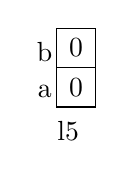
\begin{tikzpicture}
        \visible<2->{
          \draw (0.35, 0.2) node {a};
          \draw (0.5,0) rectangle (1,.5);            
        }
        \draw<4-> (.75,.25) node {0}; 
        \visible<3->{
          \draw (0.35, 0.7) node {b};
          \draw (.5,0.5) rectangle (1,1);
        }
        \draw<5-> (.75,.75) node {0};
        \visible<6->{
          \draw (.65,-.3) node {\structure{l5}};
        }
      \end{tikzpicture}        
    \end{minipage}$\!\!$\begin{minipage}[b]{.18\linewidth} %% l9
      \visible<7->{
        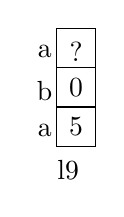
\begin{tikzpicture}
          \draw (0.35, 0.2) node {a};
          \draw (0.5,0) rectangle (1,.5);
          \draw (.75,.25) node {5};
          
          \draw (0.35, 0.7) node {b};
          \draw (.5,0.5) rectangle (1,1);
          
          \draw<5-> (.75,.75) node {0};
          
          \visible<8->{
            \draw (0.35, 1.2) node {a};
            \draw (.5,1) rectangle (1,1.5);
            \draw (.75, 1.2) node {?};
          }
          \visible<9->{
            \draw (.65,-.3) node {\structure{l9}};
          }
        \end{tikzpicture}
      }
    \end{minipage}$\!\!$\begin{minipage}[b]{.18\linewidth} %% l14
      \visible<10->{
        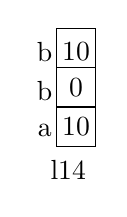
\begin{tikzpicture}
          \draw (0.35, 0.2) node {a};
          \draw (0.5,0) rectangle (1,.5);
          \draw (.75,.25) node {10};
          
          \draw (0.35, 0.7) node {b};
          \draw (.5,0.5) rectangle (1,1);
          \draw (.75,.75) node {0};
          
          \visible<11->{
            \draw (0.35, 1.2) node {b};
            \draw (.5,1) rectangle (1,1.5);
            \draw<11-> (.75, 1.2) node {10};
          }
          \visible<12->{
            \draw (.65,-.3) node {\structure{l14}};
          }          
        \end{tikzpicture}
      }
    \end{minipage}$\!\!$\begin{minipage}[b]{.18\linewidth} %% l18
      \visible<13->{
        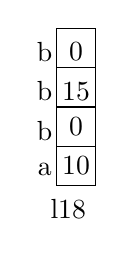
\begin{tikzpicture}
          \draw (0.35, 0.2) node {a};
            \draw (0.5,0) rectangle (1,.5);
            \draw (.75,.25) node {10};
            
            \draw (0.35, 0.7) node {b};
            \draw (.5,0.5) rectangle (1,1);
            \draw (.75,.75) node {0};

            \draw (0.35, 1.2) node {b};
            \draw (.5,1) rectangle (1,1.5);
            \draw (.75, 1.2) node {15};

            \visible<14->{
              \draw (0.35, 1.7) node {b};
              \draw (.5,1.5) rectangle (1,2);
              \draw (.75, 1.7) node {0};
            }
            \visible<15->{
              \draw (.65,-.3) node {\structure{l18}};
            }
          \end{tikzpicture}
        }
    \end{minipage}$\!\!$\begin{minipage}[b]{.18\linewidth} %% l20
        \visible<16->{
          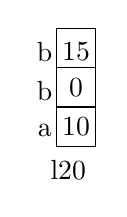
\begin{tikzpicture}
            \draw (0.35, 0.2) node {a};
            \draw (0.5,0) rectangle (1,.5);
            \draw (.75,.25) node {10};
            
            \draw (0.35, 0.7) node {b};
            \draw (.5,0.5) rectangle (1,1);
            \draw (.75,.75) node {0};
            
            \draw (0.35, 1.2) node {b};
            \draw (.5,1) rectangle (1,1.5);
            \draw (.75, 1.2) node {15};
            
            \draw (.65,-.3) node {\structure{l20}};
          \end{tikzpicture}            
        }
    \end{minipage}$\!\!$\begin{minipage}[b]{.18\linewidth} %% l22
        \visible<17->{
          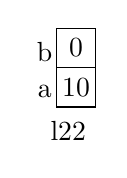
\begin{tikzpicture}
            \draw (0.35, 0.2) node {a};
            \draw (0.5,0) rectangle (1,.5);
            \draw (.75,.25) node {10};
            
            \draw (0.35, 0.7) node {b};
            \draw (.5,0.5) rectangle (1,1);
            \draw (.75,.75) node {0};
            
            \draw (.65,-.3) node {\structure{l22}};
          \end{tikzpicture}            
        }
    \end{minipage}
      
  \end{minipage}
\end{frame}
%%%%%%%%%%%%%%%%%%%%%%%%%%%%%%%%%%%%%%%%%%%%%%%%%%%%%%%%%%%%%%%%%%%%%%%%
\begin{frame}{Function Parameters}  
  \begin{block}{Parameters are stacked too}
    \begin{itemize}
    \item One \textbf{\alert{stack frame}} per function (containing local vars and parameters)
    \item Stack frame: created on function call,  destructed when the function returns
    \item Parameters can be seen as local variables (can even be modified)
    \item Parameters are \textbf{\alert{passed by value}} (ie, copied over)
    \end{itemize}
  \end{block}  

  \begin{columns}
    \begin{column}{.5\linewidth}
      \framebox{\begin{minipage}{.3\linewidth}
          \tt\footnotesize  \begin{tabbing}
            \alert<3|handout:0>{int \textbf{max}(int a, int b) \{}\\
            \alert<4|handout:0>{~~return a$>$b ? a : b;}\\
            \}\\
            \\
            \alert<1|handout:0>{int \textbf{main}() \{}\\
            \alert<1|handout:0>{~~int x=12;}\\
            \alert<1|handout:0>{~~int y=42;}\\
            \alert<5|handout:0>{~~return \alert<2|handout:0>{max(x,y);}}\\
            \}
          \end{tabbing}
        \end{minipage}}    
    \end{column}
    \begin{column}{.3\linewidth}
      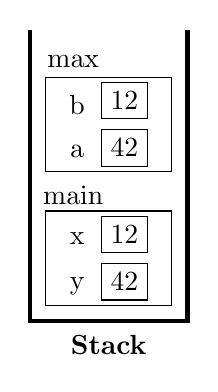
\begin{tikzpicture}
        % Stack container
        \draw[ultra thick] (0,3.7) -- (0,0) -- (2,0) -- (2, 3.7);
        \node at (1,-.3) {\bf Stack};
        
        % Stack frame of main 
        \draw (.2,.2) rectangle (1.8,1.4);
        
        \node at (1.2,.5) [shape=rectangle,draw]  {42} ;
        \node at (.6,.45) {y};
        
        \node at (1.2,1.1) [shape=rectangle,draw]  {12} ;
        \node at (.6,1.05) {x};
        
        \node at (.55,1.6) {main};
        
        \visible<3-4>{
          % Stack frame of max
          \draw (.2,1.9) rectangle (1.8,3.1);
          
          \node at (1.2,2.2) [shape=rectangle,draw]  {42} ;
          \node at (.6,2.15) {a};
          
          \node at (1.2,2.8) [shape=rectangle,draw]  {12} ;
          \node at (.6,2.75) {b};
          
          \node at (.55,3.3) {max};
        }
      \end{tikzpicture}
    \end{column}
  \end{columns}
\end{frame}
%%%%%%%%%%%%%%%%%%%%%%%%%%%%%%%%%%%%%%%%%%%%%%%%%%%%%%%%%%%%%%%%%%%%%%%%
\begin{frame}{Function Parameters Tricks}  
  \begin{block}{Parameters are passed by value}
    \begin{itemize}
    \item We just said that but it is not as natural as it seems
    \item It forbids any side effects on parameters
    \item<7> There is no way to avoid passing by value
    \item<7> But pointers help: scanf manages to ``modify its arguments''
    \end{itemize}
  \end{block}  

  \begin{columns}
    \begin{column}{.35\linewidth}
      \framebox{\begin{minipage}{.3\linewidth}
          \tt\footnotesize  \begin{tabbing}
            \alert<3|handout:0>{void \textbf{triple}(int a) \{}\\
            \alert<4|handout:0>{~~a=a*3;}\\
            \alert<5|handout:0>{~~return;}\\
            \}\\
            \\
            \alert<1|handout:0>{int \textbf{main}() \{}\\
            \alert<1|handout:0>{~~int x=12;}\\
            \alert<2|handout:0>{~~triple(x);}\\
            \alert<6|handout:0>{~~printf("x:~\%d",x);}\\
            \alert<7|handout:0>{~~return EXIT\_SUCCESS;}\\
            \}
          \end{tabbing}
        \end{minipage}}    
    \end{column}
    \begin{column}{.25\linewidth}
      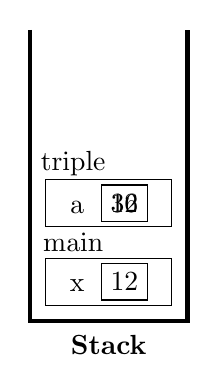
\begin{tikzpicture}
        % Stack container
        \draw[ultra thick] (0,3.7) -- (0,0) -- (2,0) -- (2, 3.7);
        \node at (1,-.3) {\bf Stack};
        
        % Stack frame of main 
        \visible<1-6>{
          \draw (.2,.2) rectangle (1.8,.8);
          
          \node at (1.2,.5) [shape=rectangle,draw]  {12} ;
          \node at (.6,.45) {x};
                
          \node at (.55,1) {main};
        }

        \visible<3-4>{
          % Stack frame of max
          \draw (.2,1.2) rectangle (1.8,1.8);
          
          \node<3|handout:0> at (1.2,1.5) [shape=rectangle,draw]  {12} ;
          \node<4> at (1.2,1.5) [shape=rectangle,draw]  {36} ;
          \node at (.6,1.45) {a};
          
          \node at (.55,2) {triple};
        }
      \end{tikzpicture}
    \end{column}
    \begin{column}{.3\linewidth}
      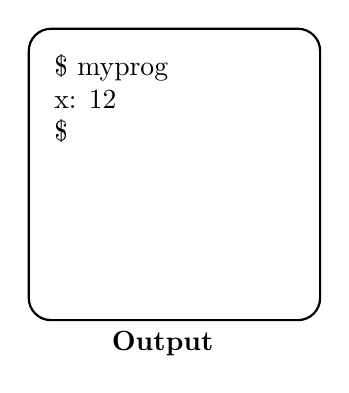
\begin{tikzpicture}
        \draw[thick,rounded corners=8pt] (0,0) rectangle (3.7,3.7);
        \node at (1.7,-.3) {\bf Output};

        \node[right] at (.2,3.2) {\$ myprog};
        \node<6->[right] at (.2,2.8) {x: 12};
        \node<7->[right] at (.2,2.4) {\$};

      \end{tikzpicture}
    \end{column}
  \end{columns}
\end{frame}
%%%%%%%%%%%%%%%%%%%%%%%%%%%%%%%%%%%%%%%%%%%%%%%%%%%
\begin{frame}{Weird Code with Function Calls}
  \vspace{-.5\baselineskip}
  \framebox{\resizebox{.4\linewidth}{!}{
  \begin{minipage}{.3\linewidth}
\footnotesize\tt  \begin{tabbing}
~1:int a;\\
~2:int main() \{\\
~3:~~int b;\\
~3:~~a=0;\\
~4:~~b=a;\\
~5:~~printab(a,b);\\
~6:~~a += 5;\\
~7:~~\{~int a;\\
~8:~~~~printab(a,b);\\
~9:~~\}\\
10:~~a += 5;\\
11:~~\{~int b=a;\\
12:~~~~printab(a,b);\\
13:~~~~b += 5;\\
14:~~~~\{~int b=0;\\
15:~~~~~~printab(a,b);\\
16:~~~~\}\\
17:~~~~printab(a,b);\\
18:~~\}\\
19:~~printab(a,b);\\
20:~~return 0;\\
21:\}\\
22:int printab(\alert<3>{int \only<1-2>{b}\only<3>{\framebox{b}}, int \only<1-2>{a}\only<3>{\framebox{a}}}) \{\\
23:~~printf("a:\%d, b:\%d$\backslash$n",a,b);~~~\\
24:\}
  \end{tabbing}          
  \end{minipage}}}\hfill%
  \begin{minipage}{.56\linewidth}
    \begin{block}{Code similar to previously}
      \begin{itemize}
      \item Call printab() for display, not printf()
      \end{itemize}
    \end{block}
    \begin{block}<2->{Old Output}\medskip
      \begin{minipage}{.5\linewidth}
        \begin{itemize}
          \item[l5] \texttt{a:~0; b:~0}
          \item[l9] \texttt{a:~??;~b:~0}
          \item[l14] \texttt{a:~10;~b:~10}
        \end{itemize}      
      \end{minipage}\begin{minipage}{.5\linewidth}
        \begin{itemize}
          \item[l18] \texttt{a:~10;~b:~0}
          \item[l20] \texttt{a:~10;~b:~15}
          \item[l22] \texttt{a:~10;~b:~0}
        \end{itemize}
      \end{minipage}      
    \end{block}

    \begin{block}<2->{New Output}\medskip
      \begin{minipage}{.5\linewidth}
        \begin{itemize}
          \item[l5] \texttt{a:0; b:0}
          \item[l9] \texttt{a:0;~b:??}
          \item[l14] \texttt{a:10;~b:10}
        \end{itemize}      
      \end{minipage}\begin{minipage}{.5\linewidth}
        \begin{itemize}
          \item[l18] \texttt{a:0;~b:10}
          \item[l20] \texttt{a:15;~b:10}
          \item[l22] \texttt{a:0;~b:10}
        \end{itemize}
      \end{minipage}      
    \end{block}
    
    \medskip\visible<2->{\concept{This is all inverted!}}

    \begin{block}<2->{The trick comes from\ldots}
      \begin{itemize}
      \item<3> printab's parameters, which are inverted
      \end{itemize}      
    \end{block}
  \end{minipage}
\end{frame}
%%%%%%%%%%%%%%%%%%%%%%%%%%%%%%%%%%%%%%%%%%%%%%%%%%%%%%%%%%%
\begin{frame}{The keyword static}
  \concept{This little keyword has two (quite differing) meanings}

  \begin{block}{When applied to global identifiers}
    \begin{itemize}
    \item \structure{Reduces visibility:} from ``the whole project'' to ``this
      file'' {\small (as if it were local)}
    \item \structure{Lifetime} remains unchanged

    \item \structure{Java equivalent:} private
    \end{itemize}
  \end{block}

  \begin{block}{When applied to local identifiers}
    \begin{itemize}
    \item \structure{Increases lifetime:} from ``for this call'' to ``for ever''
      {\small (as if it were global)}
    \item \structure{Visibility} remains unchanged
    \item \structure{Similar concept in Java:} static
    \end{itemize}
  \end{block}

  \visible<2->{
  \begin{center}
    \begin{tabular}{|l|c|c|}\cline{2-3}
      \multicolumn{1}{c|}{}      &\structure{Visibility}&\structure{Lifetime}\\\hline
      \structure{Functions}      &Whole Project&For Ever\\\hline
      \structure{Global Variable}&Whole Project&For Ever\\\hline
      \visible<3->{\structure{Static Global Variable}&This File Only&For Ever}\\\hline%visible<3->{\hline}
      \visible<3->{\structure{Static Local Variable}&Current Block&For Ever}\\\hline
      \structure{Local Variable}&Current Block&Until End of Block\\\hline      
    \end{tabular}    
  \end{center}}
\end{frame}
%%%%%%%%%%%%%%%%%%%%%%%%%%%%%%%%%%%%%%%%%%%%%%%%%%%%%%%%%%%%%%%%%%%%%%%%%
\begin{frame}{More on Static Local Variables}
  \begin{columns}
    \begin{column}{.35\linewidth}
      \framebox{\begin{minipage}{.45\linewidth}
          \tt\footnotesize  \begin{tabbing}
            \alert<3,8|handout:0>{int \textbf{nextInt}() \{}\\
            \alert<3|handout:0>{~~\alert<8|handout:0>{\textbf{\textrm{static}} int res}=0;}\\
            \alert<4,9|handout:0>{~~res+=1;}\\
            \alert<5,10|handout:0>{~~return res;}\\
            \}\\
            \\
            \alert<1|handout:0>{int \textbf{main}() \{}\\
            \alert<6|handout:0>{~~printf("next:\%d",\alert<2|handout:0>{nextInt()});}\\
            \alert<11|handout:0>{~~printf("next:\%d",\alert<7|handout:0>{nextInt()});}\\
            \alert<12|handout:0>{~~return EXIT\_SUCCESS;}\\
            \}
          \end{tabbing}
        \end{minipage}}    
    \end{column}
    \begin{column}{.15\linewidth}
      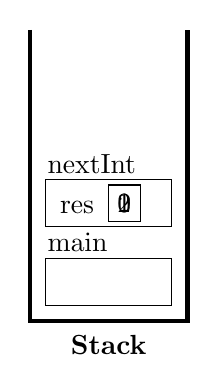
\begin{tikzpicture}
        % Stack container
        \draw[ultra thick] (0,3.7) -- (0,0) -- (2,0) -- (2, 3.7);
        \node at (1,-.3) {\bf Stack};
        
        % Stack frame of main 
        \visible<1-11>{
          \draw (.2,.2) rectangle (1.8,.8);
          \node[right] at (.1,1) {main};
        }

        \visible<3-5,8-9>{
          % Stack frame of nextInt
          \draw (.2,1.2) rectangle (1.8,1.8);
          
          \node<3|handout:0> at (1.2,1.5) [shape=rectangle,draw]  {0} ;
          \node<4-5,8|handout:0> at (1.2,1.5) [shape=rectangle,draw]  {1} ;
          \node<9-10> at (1.2,1.5) [shape=rectangle,draw]  {2} ;
          \node at (.6,1.45) {res};
          
          \node[right] at (.1,2) {nextInt};
        }
      \end{tikzpicture}
    \end{column}
    \begin{column}{.24\linewidth} 
      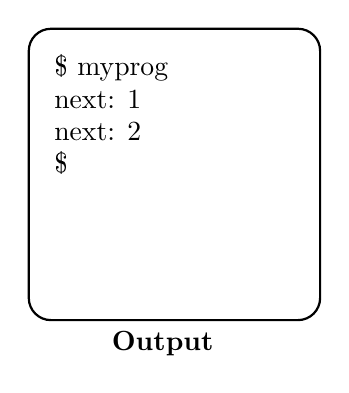
\begin{tikzpicture}
        \draw[thick,rounded corners=8pt] (0,0) rectangle (3.7,3.7);
        \node at (1.7,-.3) {\bf Output};

        \node[right] at (.2,3.2) {\$ myprog};
        \node<6->[right] at (.2,2.8) {next: 1};
        \node<11->[right] at (.2,2.4) {next: 2};
        \node<12->[right] at (.2,2) {\$};

      \end{tikzpicture}
    \end{column}
  \end{columns}

  \begin{itemize}
  \item<8-> The value remains from one call to another (initializer evaluated only once)
  \item<12-> This variable cannot live on the stack: would have been erased by
    another call
  \item<12-> Understanding where it lives require some more background on the
    system\\
    {(actually, the globals are not on the stack either)}
  \end{itemize}
\end{frame}
%%%%%%%%%%%%%%%%%%%%%%%%%%%%%%%%%%%%%%%%%%%%%%%%%%%%%%%%%%%%%%%%%%%%%%%%%%%%%%%%%%%%
\subsection{Processes Memory Layout}
\begin{frame}{Processes Memory Layout}
  \begin{block}{Primer from Next Year in System Course}
    \begin{itemize}
    \item The memory of each process is split in 3 big \textbf{\alert{segments}}
    \item Heap is for the manually managed memory (see in half an hour)
    \item<2-> If more stack frames needed, the size of the stack grows toward
      the heap\\
      Conversely, the heap can grow toward the stack
    \item<3-> Between Heap and Stack, there is a hole \visible<4->{in the
        addressing space}
    \item<3-> If that hole becomes full (stack reaches heap), the process runs out of memory
    \item This is a simplification, but the ideas are there
    \end{itemize}

    \begin{center}
    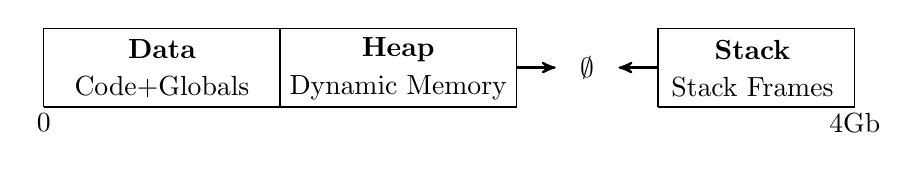
\begin{tikzpicture}
      \draw (0,0) -- (6,0) -- (6,1) -- (0,1) -- (0,0);
      \draw (7.8,0) -- (10.3,0) -- (10.3,1) -- (7.8,1) -- (7.8,0);
      \draw (3,0) -- (3,1);
      \node at (1.5,0.73) {\textbf{Data}};
      \node at (1.5,0.25) {Code+Globals};

      \node at (4.5,0.73) {\textbf{Heap}};
      \node at (4.5,0.25) {Dynamic Memory};

      \node at (9,0.73) {\textbf{Stack}};
      \node at (9,0.25) {Stack Frames};
      \visible<2->{
        \draw[-stealth',thick] (6,.5) -- (6.5,.5);
        \draw[-stealth',thick] (7.8,.5) -- (7.3,.5);
      }
      
      \node<3-> at (6.9,.5) {$\emptyset$};
      \visible<4->{        
        \node at (0,-.2) {0};
        \node at (10.3,-.2) {4Gb};
      }
    \end{tikzpicture}
    \end{center}
  \end{block}\vspace{-1.5\baselineskip}

  \begin{block}<5->{Where do symbols live?}\medskip
    \begin{minipage}{.4\linewidth}
      \begin{itemize}
      \item \structure{Functions:} in Data segment
      \item \structure{Globals:} in Data segment\\
        ~
      \end{itemize}      
    \end{minipage}~%
    \begin{minipage}{.6\linewidth}
      \begin{itemize}
      \item \structure{Locals:} in Stack segment
      \item \structure{Static Locals:} in Data segment\\
        {\small(just like globals!)}
      \end{itemize}      
    \end{minipage}~
  \end{block}
\end{frame}
%%%%%%%%%%%%%%%%%%%%%%%%%%%%%%%%%%%%%%%%%%%%%%%%%%%%%%%%%%%%%%%%%%%%%
\subsection{Addresses}
\begin{frame}{More on Memory}
  \begin{block}{Solving the Enigma of Static Locals Storage raises New Questions}
    \begin{itemize}
    \item What is the addressing space?
      \visible<2->{\structure{$\leadsto$ This is another name for ``memory''}}
    \item How to get a valid mental representation of the memory?\\
      \visible<3->{\structure{$\leadsto$ Think of a very large array of
          cells. Each cell is 1 byte (8 bits) wide.}
      \begin{center}
        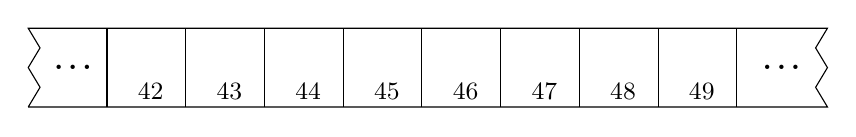
\begin{tikzpicture}
          \draw(0,0) -- (10.15,0) -- (10,.25) -- (10.15,.5) -- (10,.75) --
               (10.15,1) -- (0,1) -- (.15,.75) -- (0,.5) -- (.15,.25) -- (0,0);
          \foreach \i in { 1,2,3,4,5,6,7,8,9 } {
            \draw(\i,0) -- (\i,1);
          }
          \node at (.6,.5) {\textbf{\ldots}};
          \node at (9.6,.5) {\textbf{\ldots}};
          \visible<4->{
            \foreach \i in { 1,2,3,4,5,6,7,8 } {
              \node at (\i+.5,0.2) {\small \pgfmathtruncatemacro{\res}{41pt+\i} \res};;
            }
          }
        \end{tikzpicture}        
      \end{center}}
    \item What is an address?
      \visible<4->{\structure{$\leadsto$ Memory cells are numbered.\\ 
          The \textbf{\alert{address}} of a given memory cell is its number in rank}}
    \item Why the stack bottom at 4Gb? \visible<5->{\structure{$\leadsto$
          Because this is MAXINT on 32bits\\
          And the picture supposed that we were in 32bits for simplicity sake. }}
    \item Where is my stack if my laptop does not have 4Gb?
      \begin{itemize}
      \item<6-> \structure{Within the process, we are speaking of \textit{virtual
          addresses}}
      \item<6-> \structure{They get converted into \textit{physical ones} by the OS}
      \item<6-> \structure{But this all is to be seen in RSA (not even RS --
          end of next year)}
      \end{itemize}
    \end{itemize}
  \end{block}
\end{frame}
%%%%%%%%%%%%%%%%%%%%%%%%%%%%%%%%%%%%%%%%%%%%%%%%%%%%%%%%%%%%%%%%%%%%%%%%%%%%%%%%%%%%%%%%%
\begin{frame}{Storing Data in Memory}
  \begin{block}{What can get stored in a Memory Cell?}
    \begin{itemize}
    \item It's 8 bits long, so it can take $2^8$ values
    \item The value range is thus $[0;255]$ (or $[-127;128]$ if signed)
    \end{itemize}
  \end{block}
  \begin{block}{How to store bigger values?}
    \begin{itemize}
    \item For that, we aggregate memory cells, \textit{i.e.} we interpret
      together adjacent cells
    \item \texttt{int} are stored on 4 cells
      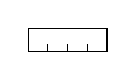
\begin{tikzpicture}
        \draw (0,0) rectangle (1,0.3);
        \foreach \i in {.25,.5,.75} {
          \draw (\i,0) -- (\i,.1);
        }
      \end{tikzpicture}
      Resulting range: $[0;2^{8\times 4}[=[0;2^{32}[\approx[0;4e^{10}]$
    \item \texttt{short} are stored on 2 cells
      \begin{tikzpicture}
        \draw (0,0) rectangle (.5,0.3);
        \foreach \i in {.25} {
          \draw (\i,0) -- (\i,.1);
        }
      \end{tikzpicture}
      ~Resulting range: $[0;2^{16}[=[0;65\,535]$
    \end{itemize}
  \end{block}

  \begin{block}{\alert{Problem}}
    \begin{itemize}
    \item \alert{Impossible to interpret a memory area without infos on data type stored}
    \item \structure{Remember:} C memory is a big magma (never forget!)
    \item Veeery different from Java where you have introspection abilities
    \end{itemize}
  \end{block}
\end{frame}
%%%%%%%%%%%%%%%%%%%%%%%%%%%%%%%%%%%%%%%%%%%%%%%%%%%%%%%%%%%%%%%%%%%%%%%%%%%
\section{Pointers}\toc
\subsection{Basics}
\begin{frame}{Pointers}
  \begin{block}{What is it?}
    \begin{itemize}
    \item \alert{Variable storing a memory address:} Pointer value = rank of a
      memory cell
    \item On 32 bits, I need 4 bytes to store an address since biggest
      address=$2^{32\times8}$\\  (8 bytes on 64 bits)
    \item Pointers are often written in hexadecimal (just a convention)
    \item Most of the time, numerical value is meaningless; where it points
      to is crucial

      \begin{center}
        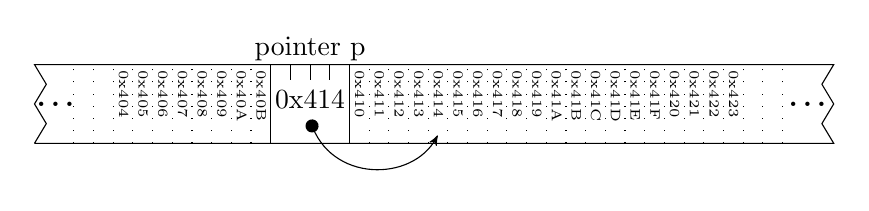
\begin{tikzpicture}
          % Base line memory area
          \draw(0,0) -- (10.15,0) -- (10,.25) -- (10.15,.5) -- (10,.75) --
               (10.15,1) -- (0,1) -- (.15,.75) -- (0,.5) -- (.15,.25) -- (0,0);
          \foreach \i in { 1,2,4,5,6,7,8 } {
            \draw[loosely dotted](\i,0)     -- (\i,1);
            \draw[loosely dotted](\i+.25,0) -- (\i+.25,1);
            \draw[loosely dotted](\i+.5,0)  -- (\i+.5,1);
            \draw[loosely dotted](\i+.75,0) -- (\i+.75,1);
            \foreach \j in {0,1,2,3} {
              \node[right,rotate=270] at (\i+.13+\j*.25,1.05) 
                {\tiny 0x\pgfmathtruncatemacro{\res}{1024pt+(\i*4)+\j}%
                  \pgfmathdectoBase\mynumber{\res}{16}\mynumber};
            }
          }
          \foreach \i in {.25,.5,.75} {
            \draw(3+\i,1) -- (3+\i,.8);
          }
          \draw[loosely dotted](.5,0)   -- (.5,1); 
          \draw[loosely dotted](.75,0)  -- (.75,1); 
          \draw[loosely dotted](9,0)    -- (9,1); 
          \draw[loosely dotted](9.25,0) -- (9.25,1);
          \draw[loosely dotted](9.5,0)  -- (9.5,1);

          \node at (.3,.5) {\textbf{\ldots}};
          \node at (9.85,.5) {\textbf{\ldots}};

          % Example of a pointer in that memory
          \node at (3.5,1.2) {pointer p}; 
          \draw (3,0)    -- (3,1); 
          \draw (4,0)    -- (4,1); 

          \node at (3.5,.55) {0x414};
          \draw[*-stealth'] (3.5,0.3) .. controls (3.75,-0.5) and (4.8,-0.5) .. (5.12,0.1);          
        \end{tikzpicture}        
      \end{center}
    \end{itemize}
  \end{block}\vspace{-.7\baselineskip}

  \begin{block}<2->{But we can't interpret memory areas w/o info on stored type!}
    \begin{itemize}
    \item This information is given by the type of pointer
    \item[] \texttt{char* pc;}
      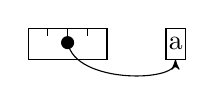
\begin{tikzpicture}[baseline]
        \draw (0,0) rectangle (1,0.4);
        \foreach \i in {.25,.5,.75} {
          \draw (\i,.3) -- (\i,.4);
        }

        \draw (1.75,0) rectangle (2,.4);
        \node at (1.87,0.2) {a};

        \draw[*-stealth'] (.5,0.3) .. controls (.5,-0.3) and (1.87,-0.3) .. (1.87,0);
      \end{tikzpicture}
      \hspace{2em}
      \texttt{int* pi;}
      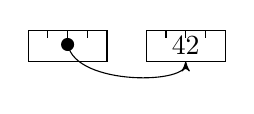
\begin{tikzpicture}[baseline]
        \draw (0,0) rectangle (1,0.4);
        \foreach \i in {.25,.5,.75,  1.75,2,2.25} {
          \draw (\i,.3) -- (\i,.4);
        }

        \draw (1.5,0) rectangle (2.5,.4);
        \node at (2,0.2) {42};

        \draw[*-stealth'] (.5,0.3) .. controls (.5,-0.3) and (2,-0.3) .. (2,0);
      \end{tikzpicture}
    \item It is possible to store the address of a pointer of a pointer:
      \texttt{int ***p;}\\
      \structure{Remember:} types are to be read from right to left
    \end{itemize}
  \end{block}
\end{frame}
%%%%%%%%%%%%%%%%%%%%%%%%%%%%%%%%%%%%%%%%%%%%%%%%%%%%%%%%%%%%%%%%%%%%%%%%
\begin{frame}{Pointers Pitfalls}
  \Concept{There is reasons why students don't like pointers}
  \medskip

  \begin{block}{Pitfall \#1: * has a very heavy semantic}
    \begin{itemize}
    \item This little char is very loaded of semantic in C
    \item Forget only one * somewhere, and you're running into the segfault\\
      Same thing when writing a * too much
    \end{itemize}
  \end{block}\vspace{-.5\baselineskip}

  \begin{block}{Pitfall \#2: * actually has two differing meanings}
    \begin{itemize}
    \item \framebox{\texttt{int *p}} declares a \textbf{\alert{pointer
          variable}} \texttt{p} which is a pointer to an integer value
    \item \framebox{\texttt{*p}} is then the \textbf{\alert{pointed value}},
      interpreted according to the pointer type
    \item (that's actually three meanings when counting $\times$, the multiplication)
      \medskip
    \item \framebox{\texttt{int *p; p=12;}} selects where it points in memory
    \item \framebox{\texttt{int *p; *p=12;}} changes the memory in the pointed area
      \medskip

    \item Pascal was a bit more reasonable: \framebox{\texttt{INTEGER \^{}p}}
      vs. \framebox{\texttt{p\^{}}} {\small(at least other order)}
    \item In Java, there is no pointers, but reference to objects are close to
      that concept
    \end{itemize}
  \end{block}
\end{frame}
%%%%%%%%%%%%%%%%%%%%%%%%%%%%%%%%%%%%%%%%%%%%%%%%%%%%%%%%%%%%%%%%%%%%%%%%%%%%%%%%%%%%%%
\begin{frame}{Retrieving the address of something}
  \begin{block}{Motivation}
    \begin{itemize}
    \item Knowing that your pointer \texttt{p} points to 0x2342 is almost never relevant
    \item Knowing that it points to your variable \texttt{i} is what you need
    \end{itemize}
  \end{block}\vspace{-.5\baselineskip}
  \begin{block}{This is what the \alert{\&} operator does}
    \begin{itemize}
    \item \texttt{int i=42; \visible<2->{int *p=\alert{\&}i;}}
      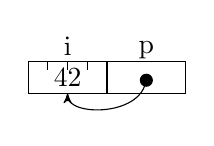
\begin{tikzpicture}[baseline]
        \draw (0,0) rectangle (1,0.4);
        \foreach \i in {.25,.5,.75} {
          \draw (\i,.3) -- (\i,.4);
        }
        \node at (.5,0.2) {42};
        \node at (.5,.6) {i};

        \visible<2->{
          \draw (1,0) rectangle (2,.4);
          \foreach \i in {.25,.5,.75} {
            \draw (\i,.3) -- (\i,.4);
          }
          \draw[*-stealth'] (1.5,0.25) .. controls (1.5,-0.3) and (.5,-0.3) .. (.5,0);
          \node at (1.5,.55) {p};
        }        
      \end{tikzpicture}
      \visible<2->{\footnotesize(successive variables are (often) adjacent)}
    \end{itemize}
  \end{block}\vspace{-.5\baselineskip}

  \begin{block}<3->{We can now explain how scanf ``modifies its arguments''}
%    \medskip
    \begin{columns}
      \begin{column}{.2\linewidth}
\framebox{\tt\scriptsize\begin{minipage}{.5\linewidth}
\begin{tabbing}
int main() \{\\
~~int a;\\
~~scanf("\%d",\alert{\&}a);\\
\}
  \end{tabbing}    
  \end{minipage}}
      \end{column}
      \begin{column}{.2\linewidth}
      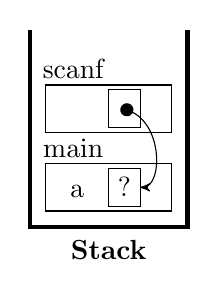
\begin{tikzpicture}
        % Stack container
        \draw[ultra thick] (0,2.5) -- (0,0) -- (2,0) -- (2, 2.5);
        \node at (1,-.3) {\bf Stack};
        
        % Stack frame of main 
        \draw (.2,.2) rectangle (1.8,.8);
        
        \node at (1.2,.5) [shape=rectangle,draw]  {?} ;
        \node at (.6,.45) {a};
                
        \node at (.55,1) {main};

        % Stack frame of scanf
        \draw (.2,1.2) rectangle (1.8,1.8);
          
        \node at (1.2,1.5) [shape=rectangle,draw]  {\phantom{?}} ;          
        \node at (.55,2) {scanf};

        \draw[*-stealth'] (1.15,1.5) .. controls (1.7,1.4) and (1.7,.5) .. (1.4,.5);

      \end{tikzpicture}
        
      \end{column}
      \begin{column}{.6\linewidth}
        \begin{itemize}
        \item \texttt{scanf} parameter: an address\\
          "\%d" tells how to interpret it
        \item That's copied over, but that's fine
        \item \texttt{scanf} can modify the \texttt{a} variable,\\
          even if it's not in its scope\\
          (\structure{remember:} C memory is a magma)
        \item other mystery: \visible<4->{variable amount of params\\
          \framebox{\texttt{man stdarg}} ;)}
        \end{itemize}
      \end{column}
    \end{columns}
  \end{block}
\end{frame}
%%%%%%%%%%%%%%%%%%%%%%%%%%%%%%%%%%%%%%%%%%%%%%%%%%%%%%%%%%%%%%%%%%%%%%%%%%%%%%%%%%%%%%%%%%%%
\newcommand{\strongstar}{\textbf{\textrm{*}}}
\begin{frame}{Fixing the triple() function}
  \begin{itemize}
  \item Remember our broken triple() function, which were unable to triple its argument
  \item That was because parameters are passed by value (copied over)
  \item To fix it, we simply use a pointer parameter
  \end{itemize}
    \begin{columns}
    \begin{column}{.35\linewidth}
      \framebox{\begin{minipage}{.3\linewidth}
          \tt\footnotesize  \begin{tabbing}
            \alert<3|handout:0>{void \textbf{triple}(int \strongstar a) \{}\\
            \alert<4|handout:0>{~~\strongstar a=(\strongstar a)*3;}\\
            \alert<5|handout:0>{~~return;}\\
            \}\\
            \\
            \alert<1|handout:0>{int \textbf{main}() \{}\\
            \alert<1|handout:0>{~~int x=12;}\\
            \alert<2|handout:0>{~~triple(\&x);}\\
            \alert<6|handout:0>{~~printf("x:~\%d",x);}\\
            \alert<7|handout:0>{~~return EXIT\_SUCCESS;}\\
            \}
          \end{tabbing}
        \end{minipage}}    
    \end{column}
    \begin{column}{.25\linewidth}
      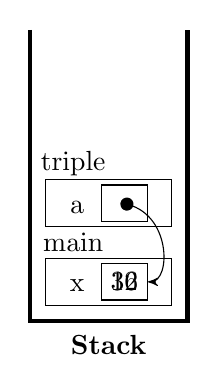
\begin{tikzpicture}
        % Stack container
        \draw[ultra thick] (0,3.7) -- (0,0) -- (2,0) -- (2, 3.7);
        \node at (1,-.3) {\bf Stack};
        
        % Stack frame of main 
        \visible<1-6>{
          \draw (.2,.2) rectangle (1.8,.8);
          
          \node<-3|handout:0> at (1.2,.5) [shape=rectangle,draw]  {12} ;
          \node<4-> at (1.2,.5) [shape=rectangle,draw]  {36} ;
          \node at (.6,.45) {x};
                
          \node at (.55,1) {main};
        }

        \visible<3-4>{
          % Stack frame of max
          \draw (.2,1.2) rectangle (1.8,1.8);
          
          \node at (1.2,1.5) [shape=rectangle,draw]  {\phantom{36}} ;
          \node at (.6,1.45) {a};
          \draw[*-stealth'] (1.15,1.5) .. controls (1.8,1.4) and (1.8,.5) .. (1.5,.5);
          
          \node at (.55,2) {triple};
        }
      \end{tikzpicture}
    \end{column}
    \begin{column}{.3\linewidth}
      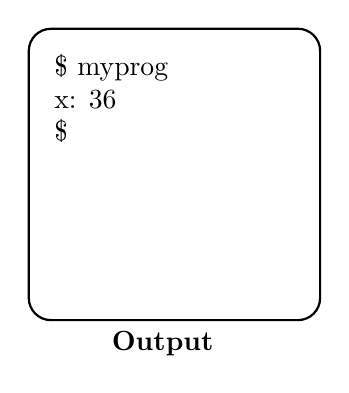
\begin{tikzpicture}
        \draw[thick,rounded corners=8pt] (0,0) rectangle (3.7,3.7);
        \node at (1.7,-.3) {\bf Output};

        \node[right] at (.2,3.2) {\$ myprog};
        \node<6->[right] at (.2,2.8) {x: 36};
        \node<7->[right] at (.2,2.4) {\$};

      \end{tikzpicture}
    \end{column}
  \end{columns}
  \begin{itemize}
  \item<7-> Pointers are powerful tools (that's why they are dangerous)
  \end{itemize}
\end{frame}
%%%%%%%%%%%%%%%%%%%%%%%%%%%%%%%%%%%%%%%%%%%%%%%%%%%%%%%%%%%%%%%%%%%%%%%%%%%%%%%%%%%
\subsection{Pointers vs. Arrays}
\begin{frame}{Pointers vs. Arrays}
  \begin{block}{In C, \alert{Arrays are Pointers} (at least, most of the time)}
    \begin{itemize}
    \item Unfortunate heritage of C first years; One of the major pitfall for newcomers
    \item \framebox{\texttt{char name[32];}} pointer to a \textbf{reserved} area of 32
      bytes
    \item \framebox{\texttt{int ai[~] = \{0,1,2\};}} pointer to a reserved and
      inited area of 3 ints
    \item \framebox{\texttt{void max(int ai[~])}} $\approx$
      \framebox{\texttt{void max(int *ai)}}  Expects an int pointer 
    \item \framebox{\texttt{void max(int ai[32])}} Similar, but whole array is
      copied on stack
    \item When using \texttt{name} after \framebox{\texttt{char name[32]}} as
      if it were an automatic \&\\
      {\texttt{name}, when looked at as pointer, is the address of the first
        array cell}
    \item This explains why strings don't take any \& in scanf: they already
      are pointers
    \end{itemize}
  \end{block}

  \begin{block}{Considering Pointers as Arrays}
    \begin{itemize}
    \item \framebox{\texttt{int *pi=}\ldots\texttt{; pi[3];}} This is valid;
      Behave as expected\\
      {\small (no bound checking, as usual in C)}
    \end{itemize}
  \end{block}

\end{frame}
%%%%%%%%%%%%%%%%%%%%%%%%%%%%%%%%%%%%%%%%%%%%%%%%%%%%%%%%%%%%%%%%%%%%%%%%%%%%%%%%%%%
\begin{frame}{Pointer Arithmetic}
  \begin{block}{Adding and subtracting integers to pointers is valid} 
    \begin{itemize}
    \item It represents a \textbf{\alert{shift in cell (not in bytes)}}
    \end{itemize}
  \end{block}
  \begin{columns}
    \begin{column}{.25\linewidth}
      \framebox{\begin{minipage}{.3\linewidth}
          \tt\footnotesize  \begin{tabbing}
            int *pi=0x400;\\
            pi=pi+3;\\
            printf("pi:\%x$\backslash$n",pi);
          \end{tabbing}
        \end{minipage}}    
    \end{column}
    \begin{column}{.55\linewidth}
      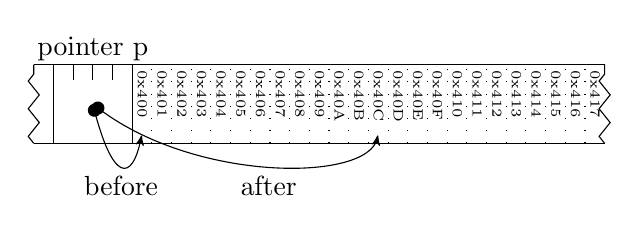
\begin{tikzpicture}[baseline]
        % Base line memory area
        \draw(.75,0) -- (8,0);
        \draw(.75,1) -- (8,1);
        \draw[decorate,decoration={zigzag,amplitude=2pt}] (.75,0) -- (.75,1);
        \draw[decorate,decoration={zigzag,amplitude=2pt}] (8,0) -- (8,1);

          \foreach \i in { 2,3,4,5,6,7 } {
            \draw[loosely dotted](\i,0)     -- (\i,1);
            \draw[loosely dotted](\i+.25,0) -- (\i+.25,1);
            \draw[loosely dotted](\i+.5,0)  -- (\i+.5,1);
            \draw[loosely dotted](\i+.75,0) -- (\i+.75,1);
            \foreach \j in {0,1,2,3} {
              \node[right,rotate=270] at (\i+.13+\j*.25,1.05) 
                {\tiny 0x\pgfmathtruncatemacro{\res}{1016pt+(\i*4)+\j}%
                  \pgfmathdectoBase\mynumber{\res}{16}\mynumber};
            }
          }
          \foreach \i in {.25,.5,.75} {
            \draw(1+\i,1) -- (1+\i,.8);
          }

          % Example of a pointer in that memory
          \node at (1.5,1.2) {pointer p}; 
          \draw (1,0)    -- (1,1); 
          \draw (2,0)    -- (2,1); 

          \draw[*-stealth'] (1.5,0.5) .. controls (1.75,-0.5) and (2,-0.5).. (2.12,0.1)
            node[midway,below] {before};          
          \draw[*-stealth'] (1.5,0.5) .. controls (2.75,-0.5) and (5,-0.5).. (5.12,0.1)
            node[midway,below] {after};          
      \end{tikzpicture}
    \end{column}    
  \end{columns}
  \begin{itemize}
  \item Value change in *pi:  \texttt{value\_after}= \texttt{value\_before}+\texttt{sizeof(int)}$\times3$\\
    because it points on integers
  \end{itemize}
  \begin{block}{Subtracting 2 pointers is valid} 
    \begin{itemize}
    \item It gives the shift between them (in cells, not in byte)
    \end{itemize}
  \end{block}

  \concept{Other arithmetic operations are \textbf{not valid} on pointers}

  \begin{block}{Pointers, Arithmetic, and Arrays}
    \begin{itemize}
    \item \framebox{\texttt{p[i]}} is equivalent to \framebox{\texttt{*(p+i)}}
      ~~~(yes, C notations about arrays are messy)
    \end{itemize}
  \end{block}
\end{frame}
%%%%%%%%%%%%%%%%%%%%%%%%%%%%%%%%%%%%%%%%%%%%%%%%%%%%%%%%%%%%%%%%%%%%%%%%%%%%%%%%%%%
\subsection{Casting Pointers}\subtoc
\begin{frame}{Casting Data}
  \vspace{-.5\baselineskip}
  \begin{block}{What is it?}
    \begin{itemize}\vspace{-.2\baselineskip}
    \item This is the well known \framebox{\texttt{int a =}
        \textbf{(int)}\texttt{b}} notation. More generally, \framebox{\texttt{(type)}}
    \item It is used to convert something in a type into something else
    \item Two meanings, depending on whether it's applied on scalars or
      pointers
    \item Quite the same story in Java, actually
    \end{itemize}
  \end{block}\vspace{-.5\baselineskip}

  \begin{block}{Casting Scalars: Converting values}
    \begin{itemize}\vspace{-.2\baselineskip}
    \item \texttt{double d = 5.7;} ~~~~
      \visible<2->{
        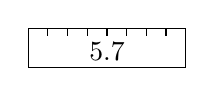
\begin{tikzpicture}[baseline]
          \draw (0,0) rectangle (2,0.5);
          \foreach \i in {.25,.5,.75,1,1.25,1.5,1.75} {
            \draw (\i,0.5) -- (\i,.4);
          }
          \node at (1,.2) {5.7};
      \end{tikzpicture}}

      \texttt{int i = (int)d;} ~~~~
      \visible<2->{
        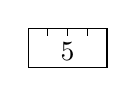
\begin{tikzpicture}[baseline]
          \draw (0,0) rectangle (1,0.5);
          \foreach \i in {.25,.5,.75} {
            \draw (\i,0.5) -- (\i,.4);
          }
          \node at (.5,.2) {5};
      \end{tikzpicture}}

    \item<2-> Casting Scalars can lead to:
      \begin{itemize}
      \item Change the memory representation of the value
      \item Change the amount of memory needed to represent the value
      \item Lead to precision loss (!)
      \end{itemize}
    \end{itemize}
  \end{block}\vspace{-.5\baselineskip}

  \begin{block}<3->{Casting Pointers: Changing the semantic}
    \begin{itemize}\vspace{-.2\baselineskip}
    \item It's written exactly the same way \ldots\ but the meaning is very different
    \item Let's look again at the Java semantic of reference casting
    \end{itemize}
  \end{block}
\end{frame}
%%%%%%%%%%%%%%%%%%%%%%%%%%%%%%%%%%%%%%%%%%%%%%%%%%%%%%%%%%%%%%%%%%%%%%%%
\begin{frame}{Casting Objects in Java}
  \begin{block}{Java Semantic Casting}
    \begin{columns}
      \begin{column}{.3\linewidth}
        \framebox{\begin{minipage}{.3\linewidth}
            \tt\footnotesize  
            \begin{tabbing}
Toto to = new Tutu();\\
Tutu tu = (Tutu)to;
            \end{tabbing}      
          \end{minipage}}
      \end{column}

      \begin{column}{.3\linewidth}
        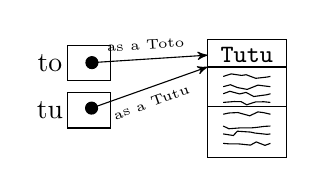
\begin{tikzpicture}[decoration={random steps,amplitude=1pt,segment length=3pt}]%[show background grid]
          % Object
          \draw (2,-.5) rectangle (3,1);
          \node at (2.5,.8) {\small\tt Tutu};
          \draw (2,.65) -- (3,.65);
          \foreach \y in {.53,.4,.31,.2,  .05,-.1,-.2,-.32} {
            \draw[decorate] (2.2,\y) -- (2.8,\y);
          }
          \draw (2,.15) -- (3,.15);
          
          % Variables
          \node at (0 ,.1) {tu};
          \node[shape=rectangle,draw] at (.5,.1) {\phantom{to}};
          
          \node at (0 ,.7) {to};
          \node[shape=rectangle,draw] at (.5,.7) {\phantom{to}};
          
          % References
          \draw[*-stealth'] (0.45,.1) -- (2,.65)
             node[sloped,midway,below] {\tiny as a Tutu};
          \draw[*-stealth'] (0.45,.7) -- (2,.8) 
             node[sloped,midway,above] {\tiny as a Toto};
        \end{tikzpicture}
      \end{column}
    \end{columns}
    
    \begin{itemize}
    \item Through \texttt{tu}, I consider the object to be a \texttt{Tutu}
    \item It does not change the value of the object, only what I expect from it
    \item Only valid if \texttt{Tutu extends Toto} (and useless if \texttt{Toto extends Tutu})
    \end{itemize}    
  \end{block}
  \begin{block}{Side note: Static vs. Dynamic typing is a creepy part of Java}
    \begin{itemize}
    \item Casts relax constraints at compilation time; Enforced at execution time\\
      That is what \texttt{TypeCastException} is made for
    \item Guessing which method gets called is sometimes excessively
      difficult\\
      {\small Check again TD4 of POO if you forgot}
    \item But it's hard to depreciate the Java typing system in a course on C\ldots
    \end{itemize}
  \end{block}
\end{frame}
\end{Coupe}
%%%%%%%%%%%%%%%%%%%%%%%%%%%%%%%%%%%%%%%%%%%%%%%%%%%%%%%%%%%%%%%%%%%%%%%%%%%%%%%%%%%%%%
\begin{frame}{Casting Pointers in C}
  \begin{block}{They change the Pointer Semantic}
    \begin{itemize}
    \item The numeric value of the pointer does not change
    \item But the dereferencing it completely different
    \item Also has a huge impact on pointer arithmetic
    \end{itemize}
  \end{block}

  \begin{columns}
    \begin{column}{.25\linewidth}
      \framebox{\begin{minipage}{.3\linewidth}
          \tt\footnotesize  \begin{tabbing}
            int a;\\
            int *pi=\&a;\\
            char *pc=pi;\\
            pi++;\\
            pc++;
          \end{tabbing}
        \end{minipage}}    
    \end{column}
    \begin{column}{.55\linewidth}
      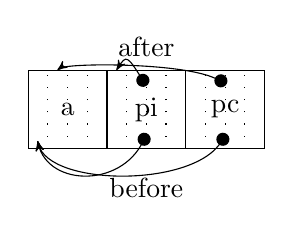
\begin{tikzpicture}[baseline]
        \foreach \cell in {1,2,3} {
          \foreach \i in {.25,.5,.75} {
            \draw[loosely dotted] (\cell+\i,0) -- (\cell+\i,1);
            \draw (\cell,0) rectangle (\cell+1,1); 
          }
        }
        
        \node at (1.5,.5) {a}; 
        \node at (2.5,.5) {pi}; 
        \node at (3.5,.5) {pc}; 


        \draw[*-stealth'] (2.5,0.2) .. controls (2.25,-0.5) and (1.25,-0.5).. (1.12,0.1);
        \draw[*-stealth'] (3.5,0.2) .. controls (3.25,-0.5) and
        (1.25,-0.5).. (1.12,0.1);
        \visible<2->{
          \node at (2.5,-.5) {before};

          \draw[*-stealth'] (2.5,0.8) .. controls (2.25,1.2) and (2.25,1.2).. (2.12,1);
          \draw[*-stealth'] (3.5,0.8) .. controls (3.25,1.1) and (1.5,1.1).. (1.37,1);
          \node at (2.5,1.3) {after};
        }

      \end{tikzpicture}
    \end{column}    
  \end{columns}
\end{frame}
%%%%%%%%%%%%%%%%%%%%%%%%%%%%%%%%%%%%%%%%%%%%%%%%%%%%%%%%%%%%%%%%%%%%%%%%%%%
\begin{frame}{Generic Pointers}
  \begin{block}{Generic pointers are sometimes handy}
    \begin{itemize}
    \item To describe pointers that can point to differing data\\
      \structure{Example:} in scanf, how to interpret the pointer is given by
      the format
    \item To describe pointers to \textit{raw} data (ie, you don't care about
      the pointed type)\\
      \structure{Example:} When copying memory chunk over, content does not matter
    \end{itemize}
  \end{block}
  \begin{block}{That is what void* is made for}
    \begin{itemize}
    \item Modern compiler even allow you to do pointer arithmetic on them
    \item[] supposing that \texttt{sizeof(void)=1}, which is \ldots\ arbitrary
    \item Older compiler force you to cast them to \texttt{char*} before
    \end{itemize}
  \end{block}
\end{frame}
%%%%%%%%%%%%%%%%%%%%%%%%%%%%%%%%%%%%%%%%%%%%%%%%%%%%%%%%%%%%%%%%%%%%%%%%%%%
\section{Dynamic Memory}\subtoc
\subsection{Memory Blocs and Pointers}
\begin{frame}{Dynamic Memory}
  \vspace{-.6\baselineskip}
  \begin{block}{Motivation}
    \begin{itemize}
    \item Arrays are statically sized in C (\textit{i.e.} their size must be
      known at compilation)
    \item It is forbidden to write:
      \framebox{\begin{minipage}{.3\linewidth}
          \tt\footnotesize  \begin{tabbing}
            int n;\\
            scanf("\%d",\&n);\\
            int tab[n];
          \end{tabbing}
        \end{minipage}}    
      because \texttt{n} is only known at execution
    \item (this is not true in C99, but C99 not widely spread yet)
    \end{itemize}
  \end{block}\vspace{-.6\baselineskip}

  \begin{block}{Solution}
    \begin{itemize}
    \item Directly request memory chunks from the system
    \item Manage them yourself
    \item And return them to the system when you're done
    \end{itemize}
  \end{block}\vspace{-.6\baselineskip}

  \begin{block}{Remember the Memory Layout of a Process}
    \begin{center}
    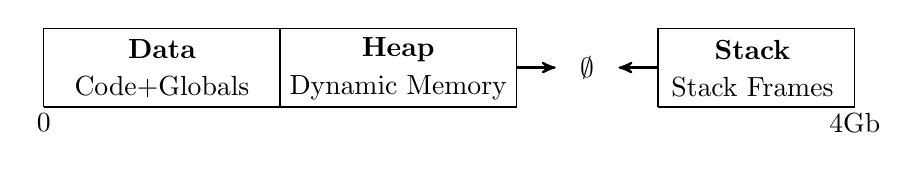
\begin{tikzpicture}
      \draw (0,0) -- (6,0) -- (6,1) -- (0,1) -- (0,0);
      \draw (7.8,0) -- (10.3,0) -- (10.3,1) -- (7.8,1) -- (7.8,0);
      \draw (3,0) -- (3,1);
      \node at (1.5,0.73) {\textbf{Data}};
      \node at (1.5,0.25) {Code+Globals};

      \node at (4.5,0.73) {\textbf{Heap}};
      \node at (4.5,0.25) {Dynamic Memory};

      \node at (9,0.73) {\textbf{Stack}};
      \node at (9,0.25) {Stack Frames};
      \draw[-stealth',thick] (6,.5) -- (6.5,.5);
      \draw[-stealth',thick] (7.8,.5) -- (7.3,.5);
      
      \node at (6.9,.5) {$\emptyset$};
      \node at (0,-.2) {0};
      \node at (10.3,-.2) {4Gb};
    \end{tikzpicture}
    \end{center}\vspace{-1.5\baselineskip}
    \begin{itemize}
    \item The idea is to request memory from the heap
    \end{itemize}
  \end{block}
\end{frame}
%%%%%%%%%%%%%%%%%%%%%%%%%%%%%%%%%%%%%%%%%%%%%%%%%%%%%%%%%%%%%%%%%%%%%%%%
\begin{frame}{Requesting Memory Chunks from the heap}
  \begin{block}{The several ways of doing so}
    \begin{itemize}
    \item As usual, there is a high level and a low level API
    \item At low-level, the \texttt{brk()} syscall allows to move the heap
      boundary\\
      And you are on your own to manage its content (emacs does it)
    \end{itemize}
  \end{block}
  \begin{block}{malloc() and friends}
    \begin{itemize}
    \item This higher level API directly gives memory chunks in heap\\
      {and deal automatically with \texttt{brk()}}
    \item There is only 3 functions to know

      \smallskip
      \begin{tabular}{rl}
      \texttt{\#include <stdlib.h>}\\
      \texttt{void*malloc(int size)}& Request a new memory chunk\\
      \texttt{void free(void*p)}& Return a memory chunk\\
      \texttt{void*realloc(void*p,int size)}& Expend a memory chunk        
      \end{tabular}
    \end{itemize}
  \end{block}
\end{frame}
%%%%%%%%%%%%%%%%%%%%%%%%%%%%%%%%%%%%%%%%%%%%%%%%%%%%%%%%%%%%%%%%%%%%%%%%
\begin{frame}{Understanding malloc and friends}
  \begin{block}{Function Semantic}
    \begin{itemize}
    \item malloc() requests a new memory chunk and return the address of beginning\\
      If there is not enough free memory, it returns NULL
    \end{itemize}
  \end{block}\vspace{-.5\baselineskip}
  \begin{block}{Think of a land registry for the memory}
    \begin{itemize}
    \item \texttt{void *A=malloc(12);}
      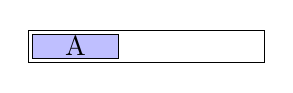
\begin{tikzpicture}[baseline]
        \draw (0,-.1) rectangle (3,.3);
        \draw[fill=blue!25] (.05,-.05) rectangle (1.15,.25) node[midway] {A};
      \end{tikzpicture}
    \item \texttt{void *B=malloc(5);~}
      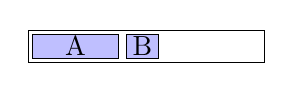
\begin{tikzpicture}[baseline]
        \draw (0,-.1) rectangle (3,.3);
        \draw[fill=blue!25] (.05,-.05)  rectangle (1.15,.25) node[midway] {A};
        \draw[fill=blue!25] (1.25,-.05) rectangle (1.65,.25) node[midway] {B};
      \end{tikzpicture}
    \item \texttt{free(A);~~~~~~~~~~~}
      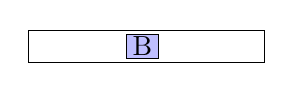
\begin{tikzpicture}[baseline]
        \draw (0,-.1) rectangle (3,.3);
        \draw[fill=blue!25] (1.25,-.05) rectangle (1.65,.25) node[midway] {B};
      \end{tikzpicture}
    \item \texttt{void *C=malloc(6);~}
      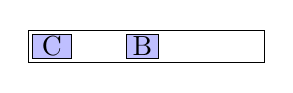
\begin{tikzpicture}[baseline]
        \draw (0,-.1) rectangle (3,.3);
        \draw[fill=blue!25] (1.25,-.05) rectangle (1.65,.25) node[midway] {B};
        \draw[fill=blue!25] (.05,-.05) rectangle (.55,.25) node[midway] {C};
      \end{tikzpicture}
    \item \texttt{C=realloc(C,13);~~~}
      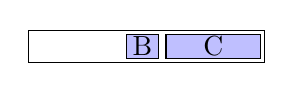
\begin{tikzpicture}[baseline]
        \draw (0,-.1) rectangle (3,.3);
        \draw[fill=blue!25] (1.25,-.05) rectangle (1.65,.25) node[midway] {B};
        \draw[fill=blue!25] (1.75,-.05) rectangle (2.95,.25) node[midway] {C};
      \end{tikzpicture}
    \end{itemize}
  \end{block}\vspace{-\baselineskip}

  \begin{block}{As usual in C}
    \begin{itemize}
    \item There is no protection mechanism here: Mess it up and you'll get a segfault
    \item Two surviving strategies:
      \begin{itemize}
      \item Avoid issues through best practices
      \item Solve issues through debugging tools
      \end{itemize}
    \end{itemize}
  \end{block}
\end{frame}
%%%%%%%%%%%%%%%%%%%%%%%%%%%%%%%%%%%%%%%%%%%%%%%%%%%%%%%%%%%%%%%%%%%%%%%%%%%%%%%%%%%
\begin{frame}{Best Practices about Dynamic Memory}
  \begin{block}{\alert{Rule \#1:} Only access to reserved areas}
    \begin{itemize}
    \item \structure{Land Registry Analogy:} Only build stuff on land that you own
    \end{itemize}
    \begin{columns}
      \begin{column}{.4\linewidth}
        \begin{center}
          \framebox{\begin{minipage}{.3\linewidth}
          \tt\footnotesize  \begin{tabbing}
            int *A;\\
            *A=1;\\
            A=malloc(sizeof(int));
          \end{tabbing}
        \end{minipage}}            

      \medskip
      \alert{Error! A used before malloc!}

      \medskip
      {\small (buy it before building)}
    \end{center}
  \end{column}
  \begin{column}{.4\linewidth}
    \begin{center}
      \framebox{\begin{minipage}{.3\linewidth}
          \tt\footnotesize  \begin{tabbing}
            int *A=malloc(sizeof(int));\\
            free(1);\\
            *A=1;
          \end{tabbing}
        \end{minipage}}            

      \medskip
      \alert{Error! A used after free!}

      \medskip
      {\small(forget it after selling it)}
    \end{center}
  \end{column}
\end{columns}\medskip
\begin{itemize}
\item You'll have similar symptoms in both case
  \begin{itemize}
  \item If you are lucky, segfault (error signaled where the fault is)
  \item If not, some memory pollution (probably a later segfault, harder to
    diagnose)
  \end{itemize}

\end{itemize}

  \end{block}
\end{frame}
%%%%%%%%%%%%%%%%%%%%%%%%%%%%%%%%%%%%%%%%%%%%%%%%%%%%%%%%%%%%%%%%%%%%%%%%%%%%%%%%%%%
\begin{frame}{Best Practices about Dynamic Memory}
  \begin{block}{\alert{Rule \#2:} To any malloc(), one and only one free()}
    \begin{itemize}
%    \item \structure{Land Registry Analogy:} Sell everything back (once)

    \item If you forget the \texttt{free()}, there is a \textbf{\alert{memory leak}}
      \begin{itemize}
      \item The system assumes that this area is used where it's not anymore
      \item Ok to have a few memleaks. Too much of them will exhaust system resources
      \item Slows everything down (swapping), and malloc() will eventually return NULL
      \end{itemize}

    \item If you call \texttt{free()} twice (\textbf{\alert{double free}}), strange things will occur

      \begin{columns}
        \begin{column}{.26\linewidth}
          \begin{center}
            \framebox{\begin{minipage}{.25\linewidth}
                \tt\footnotesize  \begin{tabbing}
                  int *A=malloc(12);\\
                  free(A);\\
                  int *\alert{B}=malloc(12);\\
                  free(A);
                \end{tabbing}
              \end{minipage}}            
          \end{center}
        \end{column}
        \begin{column}{.7\linewidth}
          $\leadsto$ Probably frees B \ldots\\
          Unfriendly if A and B are in two separate modules
        \end{column}
      \end{columns}

      \begin{itemize}
      \item That is why modern malloc implementations try to detect this situation
      \item And kill faulty program as soon as the error is detected
      \end{itemize}
    \end{itemize}


  \end{block}
\end{frame}

\part{Advanced C-Fu}\toc
%%%%%%%%%%%%%%%%%%%%%%%%%%%%%%%%%%%%%%%%%%%%%%%%%%%%%%%%%%%%%%%%%%%%%%%%%%%%%%%
\section{Modular C}
\subsection{Organizing large C projects}
\begin{frame}[fragile]{Organizing large C projects}
  \vspace{-1.2\baselineskip}
  \begin{block}{}
    \begin{itemize} 
    \item You are free in C: many ways to organize your code, nothing is enforced
    \item Get organized by yourself, or you'll get drown in your own code
    \end{itemize}
  \end{block}\vspace{-.5\baselineskip}

  \begin{block}{Guidelines for Java programmers in C %
      {\normalsize(Light and DIY object-orientation)}}
    \begin{itemize}
    \item Organize your code as several interacting classes
    \item Avoid inheritance by all means: ugly to mimick in C, often not helping
      anyway
    \item You can still get encapsulating and some of dynamic dispatch
    \item Each class becomes a module:
      \begin{itemize}
      \item A structure, grouping all fields of your class
      \item A set of functions acting on those structures (incl. constructor \&
        destructor)
      \end{itemize}
    \item Nothing is enforced; your code should remain clean %
      {\small(and your days pleasant)}
      \begin{itemize}
      \item Code readability as main objective (you are the main reader, help
        the reader)
      \end{itemize}
    \end{itemize}
  \end{block}

  \begin{block}{Forget about the performance, genericity, reusability \ldots~
      for now}
    
  \end{block}\vspace{-\baselineskip}
  \begin{quote}{}
    % Programmers waste enormous amounts of time thinking about, or worrying
    % about, the speed of noncritical parts of their programs, and these attempts
    % at efficiency actually have a strong negative impact when debugging and
    % maintenance are considered. 
    We should forget about small efficiencies, say about 97\% of the time:
    {\bf premature optimization is the root of all evil}. Yet we should not pass up
    our opportunities in that critical 3\%. \hfill{\rm --- Donald Knuth}
  \end{quote}
\end{frame}
%%%%%%%%%%%%%%%%%%%%%%%%%%%%%%%%%%%%%%%%%%%%%%%%%%%%
\begin{frame}[fragile]{The \texttt{point} module}

  \begin{block}{Changing each class into a module}
    \begin{itemize}
    \item A structure, grouping all fields of your class
    \item A set of functions acting on those structures (incl. constructor \&
      destructor)
    \end{itemize}
  \end{block}

  \begin{columns}
    \begin{column}{.25\linewidth}
      \begin{boitecode}{}
typedef struct \{
  int x, y;
\} point_t;              
      \end{boitecode}
    \end{column}
    \begin{column}{.6\linewidth}
      \begin{boitecode}{}
point_t *point_create(int x, int y);
void point_free(point_t *p);

void point_move(point_t *p, int dx, int dy);      
void point_add(point_t *p1, point_t *p2);      
      \end{boitecode}
    \end{column}
  \end{columns}

  \begin{center}
    \begin{tabular}{|l|l|}\hline
      \multicolumn{1}{|c|}{\structure{Java}}&\multicolumn{1}{c|}{\structure{C}}\\\hline
      References to objects&Pointers to structures\\\hline
      
      Methods included in object& Functions grouped by modules\\
      & Naming conventions at best\\\hline
      
      Dotted notation&Receiver as first parameter\\
      \multicolumn{1}{|c|}{\texttt{p.move(3,5)}}& 
      \multicolumn{1}{c|}{\texttt{point\_move(p, 3,5)}}\\\hline
      
      Automatic garbage collection&Manual memory handling\\\hline
    \end{tabular}
  \end{center}
\end{frame}

%%%%%%%%%%%%%%%%%%%%%%%%%%%%%%%%%%%%%%%%%%%%%%%%%%%%
\begin{frame}[fragile]{Full code of the \texttt{point} module}
  \begin{columns}
    \begin{column}{.45\linewidth}
      \begin{boitecode}{}
typedef struct \{
  int x, y;
\} point_t;              
      \end{boitecode}

      \begin{boitecode}{point\_t *{\bf point\_create}(int x, int y) \{}
  point_t *res=malloc(sizeof(point_t));
  res->x = x;
  res->y = y;
  return res;
\}
      \end{boitecode}

      \medskip
      \begin{boitecode}{void {\bf point\_free}(point\_t *p) \{}
  free(p);// plz still use a free function: 
\}         // more extensible for future
      \end{boitecode}
    \end{column}
    \begin{column}{.45\linewidth}
      \begin{boitecode}{void {\bf point\_move}(point\_t *p,\\
          \null~~~~~~~~~~~~~~~~~~~~~~ int dx, int dy) \{}
  p->x += dx; // p->x shortcut of (*p).x
  p->y += dy;
\}
      \end{boitecode}
      \medskip
      \begin{boitecode}{void {\bf point\_add}(point\_t *p1,\\
          \null~~~~~~~~~~~~~~~~~~~~point\_t *p2) \{}
  p1->x += p2->x;
  p1->y += p2->y;
\}
      \end{boitecode}
  \end{column}
  \end{columns}

  \begin{itemize}
  \item This really feels as Java, and this is a good news:
  \item You can code in C and still organize your code as you've learned

    \bigskip
  \item Missing: Hiding the implementation: How to have private methods and fields?
  \item Missing: Dynamic dispatch. Functions' pointers can simulate this.
  \item Missing: Inheritance. No easy way (but several ugly ones ;)
  \end{itemize}
\end{frame}
%%%%%%%%%%%%%%%%%%%%%%%%%%%%%%%%%%%%%%%%%%%%%%%%%%%%
\begin{frame}[fragile]{Having private methods in C modules}
  \begin{block}{The File is the Compilation Unit}
    \begin{itemize}
    \item Hidden methods must simply be marked \alert{\texttt{static}} $\Rightarrow$
      visible from that file only
    \item This older habit explains why Java forces public classes to have their
      own file
    \end{itemize}
  \end{block}

  \begin{block}{How to make parts visible from outside? With \structure{\textbf{header files}}!}
    \begin{itemize}
    \item Regular C files named \framebox{\texttt{point.\alert{h}}} containing
      structures \& function prototypes
    \item Hide your implementation $\Rightarrow$ hide the struct's content
      (\structure{\textbf{opaque structure}})
    \end{itemize}
  \end{block}

  \begin{columns}
    \begin{column}{.47\linewidth}
      \begin{boitecode}{point.h}
typedef struct point point_t;              

point_t *point_create(int x, int y);
void point_free(point_t *p);

void point_move(point_t *p, int dx, int dy);      
void point_add(point_t *p1, point_t *p2);      
      \end{boitecode}
    \end{column}

    \begin{column}{.45\linewidth}
      \begin{boitecode}{point.c}
\#include "point.h"
struct point \{
  int x,y;
\};

point_t *point_create(int x, int y) \{
  point_t *res = malloc(sizeof(point_t));
  res->x = x;
  res->y = y;
  return res;
\} 
      ...
      \end{boitecode}
    \end{column}
  \end{columns}
\end{frame}
%%%%%%%%%%%%%%%%%%%%%%%%%%%%%%%%%%%%%%%%%%%%%
\begin{frame}[fragile]{Dealing with the compiler's stupidity}
  \begin{block}{Problem: the C compiler is really prehistoric}
    \begin{itemize}
    \item Complains when symbols get redefined (even if the
      definitions match)
    \item Problem when \texttt{point.h} $\in$ \texttt{square.h} $\in$
      \texttt{main.c} and \texttt{square.h} $\in$ \texttt{main.c}
    \item \structure{\textbf{Multiple inclusion}} of \texttt{point.h} into
      \texttt{main.c}, leading to compilation error
    \end{itemize}
  \end{block}

  \begin{block}{Solution: fix the code before compiling}
    \begin{itemize}
    \item Remember: the preprocessor changes the code presented to the compiler
    \item We need to hide the subsequent inclusions of files
    \end{itemize}
  \end{block}

  \begin{columns}
    \begin{column}{.47\linewidth}
      \begin{boitecode}{point.h}
\alert{\textbf{\#ifndef POINT\_H}}
\alert{\textbf{\#define POINT\_H}}
typedef struct point point_t;              

point_t *point_create(int x, int y);
void point_free(point_t *p);

void point_move(point_t *p, int dx, int dy);      
void point_add(point_t *p1, point_t *p2);      
\alert{\textbf{\#endif /* POINT\_H */}}
      \end{boitecode}
    \end{column}

    \begin{column}{.48\linewidth}
      \begin{itemize}\vspace{-.6\baselineskip}
      \item \texttt{point.c} remains unchanged
      \item This construct seems ugly first
      \item But this is the one true way
      \item Just works, simple and efficient
      \item Not sufficient on Windows.\\
        C on Windows is pure masochism\\
        (but not because of C)
      \end{itemize}
    \end{column}
  \end{columns}
\end{frame}
%%%%%%%%%%%%%%%%%%%%%%%%%%%%%%%%%%%%%%%%%%%%%
\begin{frame}[fragile,squeeze]{Advanced OOP in C}
  \begin{block}{Dynamic dispatch}
    \begin{itemize}
    \item Structures can contain pointers to function (but shouldn't when possible)
    \end{itemize}
    \begin{columns}
      \begin{column}{.5\linewidth}
        \begin{boitecode}{}
typedef struct point *point_t; // forward decl
struct point \{
  int x, y;
  void \alert{(*display)}(point_t* p);
\} 
        \end{boitecode}
      \end{column}
      \begin{column}{.39\linewidth}
        \begin{boitecode}{}
void my_display(point_t*p) \{..\}
     ...
p1->display = &my\_display;          
     ...
(*(p1->display)) (p1); // just a call
        \end{boitecode}
      \end{column}
    \end{columns}
  \end{block}\vspace{-.3\baselineskip}

  \begin{block}{Inheritance}
    \begin{itemize}
    \item Including structures is a UGLY but working approach. \alert{Don't do
        this for real}
    \item Inheritance is over-sold anyway. You should never expose your
      inheritance tree
    \end{itemize}

    \begin{columns}
      \begin{column}{.5\linewidth}
        \begin{boitecode}{}
typedef struct particle \{
  point_t super; // whole structure copied over
  int vx, vy;
\} particle_t;
        \end{boitecode}
      \end{column}
      \begin{column}{.39\linewidth}
        \begin{boitecode}{}
void particle_animate(particle_t *mp) \{
  mp->super.x = p1->vx;
  mp->super.y = p1->vy;
\}
        \end{boitecode}
      \end{column}
    \end{columns}\vspace{-.5\baselineskip}
    \begin{itemize}
    \item Any particle can even be casted into a point to retrieve x and y
    \item But NO SAFEGUARD here. So pain to debug, impossible to read, etc.
    \item Y U NO C++ (or Objective C) if you really need OOP in C??
    \end{itemize}

  \end{block}
\end{frame}
%%%%%%%%%%%%%%%%%%%%%%%%%%%%%%%%%%%%%%%%%%%%%
\subsection{Compiling Multi-Files Projects and Makefiles}
\begin{frame}{Having many files in your project (one per module)}
  \begin{block}{That's a good habit}
    \begin{itemize}
    \item Because a 500,000 lines file is hard to navigate 
    \item Because  we can compile each of them separately
      \begin{itemize}
      \item Remember: compilation = translation into assembly lang. + linking of ASM
      \item Translation: hard and takes time; Assembling the puzzle: much faster
      \item Multiple files allows to translate only the parts that changed
      \end{itemize}
    \item Because several people can work on the same project w/o interfering
    \end{itemize}
  \end{block}\vspace{-.5\baselineskip}
  \begin{block}<2->{But harder to compile right}
    \begin{itemize}
    \item \structure{Compilation:} 
      \fbox{\small\texttt{gcc -c point.c}} 
      \fbox{\small\texttt{gcc -c square.c}} 
      \fbox{\small\texttt{gcc -c main.c}}\\[2pt]
      {\small It generates \texttt{point.o, square.o, main.o} containing the
        assembly translations}
    \item \structure{Linking:} 
      \fbox{\small\texttt{gcc -o project point.o square.o main.o}}
    \item Tracking dependencies is a nightmare \textit{e.g.} when header files
      are changed
    \item We need a specific tool for that\visible<3>{. It's called
        \structure{\textbf{make}}}
    \item<3> Even from eclipse, use makefiles. Obey the UNIX philosophy:

      \smallskip \centerline{\it Write programs that do one thing and do it
        well. Write programs to work together.}
  \end{itemize}
  \end{block}
\end{frame}

%%%%%%%%%%%%%%%%%%%%%%%%%%%%%%%%%%%%%%%%%%%%%%%%%%%%%%%%%%%%%%%%%%%%%%%%%%%%%%%
\begin{frame}[fragile]{Make and Makefiles}
  \begin{block}{Makefile: explaining the project building process}    
    \begin{itemize}
    \item Create a file named \framebox{\texttt{Makefile}} in your project,
      containing a set of rules
        {  \footnotesize
        \begin{semiverbatim}
<target file>: <list of dependencies>
    <command to build target from deps>
        \end{semiverbatim}}\vspace{-.7\baselineskip}
    \end{itemize}
  \begin{columns}
    \begin{column}{.45\linewidth}\medskip
  \begin{boitecode}{Simple Makefile}
project: point.o square.o main.o
    gcc point.o square.o main.o -o project

point.o: point.c point.h
    gcc -c point.c

square.o: square.c square.h point.h
    gcc -c square.c

main.o: main.c square.h point.h
    gcc -c main.c
  \end{boitecode}      
    \end{column}
    \begin{column}{.48\linewidth}
      \begin{boitecode}{\texttt{make} already knows to build .o from .c}
project: point.o square.o main.o
    gcc point.o square.o main.o -o project

point.o: point.c point.h
square.o: square.c square.h point.h
main.o: main.c square.h point.h
      \end{boitecode}

      \vspace{-.7\baselineskip}
      \begin{boitecode}{\texttt{make} loves funky variable names}
project: point.o square.o main.o
    gcc \$^ -o \$@
      \end{boitecode}
    \end{column}
  \end{columns}
  \end{block}
  \begin{itemize}\vspace{-.2\baselineskip}
  \item Builds first target by default; Specify another one if you want
    \framebox{\texttt{make clean}}
  \item\texttt{make} is used widely, not only for C. You could use it for you Java code!
  \end{itemize}
\end{frame}

%%%%%%%%%%%%%%%%%%%%%%%%%%%%%%%%%%
\section{The Many Ways of Messing Up in C}\subtoc
\subsection{Syntax Pitfalls}
\begin{frame}{}
  \thispagestyle{empty}
  \begin{center}
    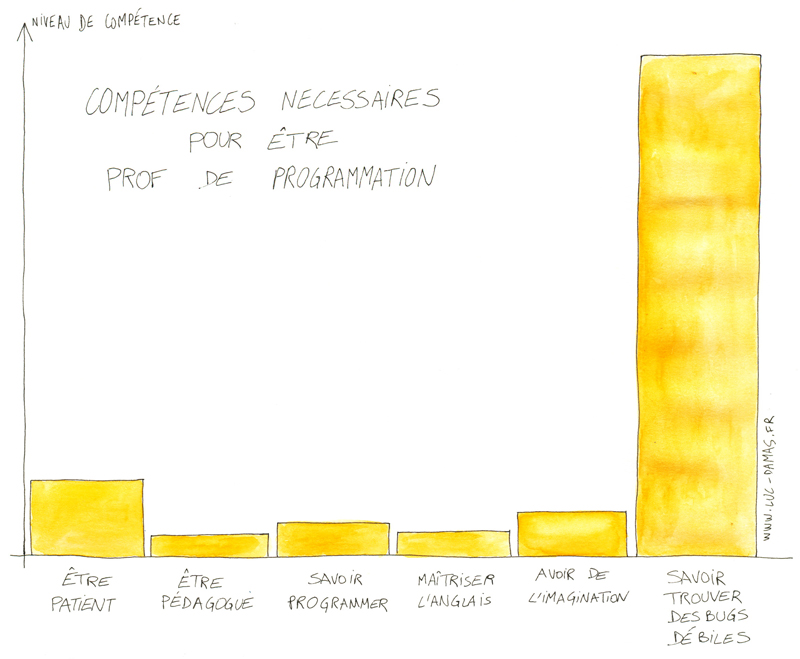
\includegraphics[width=.9\linewidth]{img/competences-prof-programmation.jpg}
    %
    \rotatebox{90}{~~~~~~~~~~~~~~~~~~~~
\includegraphics[width=7mm]{img/by-nc-sa.png}}
  \end{center}
\end{frame}

%%%%%%%%%%%%%%%%%%%%%%%%%%%%%%%%%%
\begin{frame}[fragile,squeeze]{Classical errors with the \texttt{for} loop}
  \begin{columns}
    \begin{column}{.35\linewidth}
      \begin{boitecode}{}
for (i=0; i < 10; \alert<2>{i+1})
   printf("i=\%d\n",i);
      \end{boitecode}
    \end{column}

    \begin{column}<2->{.6\linewidth}
      \begin{itemize}\vspace{-1.3\baselineskip}
      \item Y U NO increment your counter??
      \item[] (\texttt{i+1} has no side effect)
      \end{itemize}
    \end{column}
  \end{columns}

  \begin{columns}
    \begin{column}<2->{.35\linewidth}
      \begin{boitecode}{}
for (i=0; \alert<3>{i = 10}; i++) 
   printf("i=\%d\n",i);
      \end{boitecode}
    \end{column}

    \begin{column}<3->{.6\linewidth}
      \begin{itemize}\vspace{-1.3\baselineskip}
      \item Y U NO test your counter??
      \item[] (\texttt{i=10} sets a new value)
      \end{itemize}
    \end{column}
  \end{columns} 

  \begin{columns}
    \begin{column}<3->{.35\linewidth}
      \begin{boitecode}{}
for (i=0; i < 10; i++)\alert<4>{;}
   printf("i=\%d\n",i);
      \end{boitecode}
    \end{column}

    \begin{column}<4->{.6\linewidth}
      \begin{itemize}\vspace{-1.3\baselineskip}
      \item Y U NO enter your loop??
      \item[] (the \framebox{;} after the \texttt{for} closes the loop)
      \end{itemize}
    \end{column}
  \end{columns}

  \begin{columns}
    \begin{column}<4->{.35\linewidth}
      \begin{boitecode}{}
for (\alert<5>{i=0, j=0}; i < 10; i++)
   printf("i=\%d\n",i);
      \end{boitecode}
    \end{column}

    \begin{column}<5->{.6\linewidth}
      \begin{itemize}\vspace{-1.3\baselineskip}
      \item Y U NO see when it's correct??
      \item[] \framebox{,} separate expressions, \framebox{;} instructions
      \end{itemize}
    \end{column}
  \end{columns}
\end{frame}

%%%%%%%%%%%%%%%%%%%%%%%%%%
\begin{frame}[fragile]{Beware of the vicious \texttt{switch} syntax!}
  \begin{columns}
    \begin{column}{.23\linewidth}
      \begin{boitecode}{}
int x = 2;
switch(x) \{
  case 2:
    printf("Two\n");
  case 3:
    printf("Three\n");
\}     
      \end{boitecode}
    \end{column}
    \begin{column}<2->{.6\linewidth}
      \begin{itemize}
      \item Prints both: \framebox{\hbox to .32\linewidth{\vbox{\texttt{Two\\Three}}}}
      \item Problem: missing \texttt{break} keywords
      \item Because in assembly, that's a jump table
      \end{itemize}
    \end{column}
  \end{columns}

  \visible<2->{
    \begin{itemize}
    \item So that's a (sad) inheritance of assembly language
    \item And that's very sad that this propagated to Java\ldots
    \item This also explains why \texttt{case} values must be constant
    \end{itemize}
  }
\end{frame}
%%%%%%%%%%%%%%%%%%%%%%%%%%

\subsection{Understanding gcc Error Messages}
\begin{frame}[fragile]{Understanding \texttt{gcc} error messages}
  \centerline{\texttt{gcc} \textbf{is} user friendly. It's just picky about its
    friends}\smallskip
  \concept{But you \textbf{have to} pass \framebox{\texttt{-Wall -Wextra}} as parameter}

   \bigskip
   \bigskip

  \begin{block}{Suggest parentheses around assignment used as truth value\ldots}
    \bigskip\smallskip
    \begin{columns}
      \begin{column}{.1\linewidth}
        \begin{boitecode}{}
if (a=b)
        \end{boitecode}
      \end{column}
      \begin{column}<2>{.78\linewidth}
        \begin{itemize}\vspace{-1.3\baselineskip}
        \item \ldots if you \textbf{really} mean to erase a, 
          then write \framebox{if ((a=b))}
        \item Else, you probably meant \framebox{if (a==b)}
        \item The compiler gives a meaning even to the weird \framebox{if ((a=b)!=0)}
        \end{itemize}
      \end{column}
    \end{columns}
  \end{block}
\end{frame}
%%%%%%%%%%%%%%%%%%%%%%%%%%%%%%%%%%%
\begin{frame}[fragile]{Return of functions}
  \begin{itemize}
  \item \structure{\large warning: 'return' with a value, in function returning void}\\
    Yeah that's only a warning --- keep calm and add \framebox{\texttt{-Werror}}
    

    \bigskip
  \item<2-> \structure{\large Control reaches end of non void function:} self
    explanatory (?)
  \end{itemize}

  \begin{columns}
    \begin{column}<2->{.3\linewidth}
      \begin{boitecode}{\alert{\bf Don't do that}}
int my_function() \{
   if (x == 2)
      return 1;
\}

      \end{boitecode}
    \end{column}
    \begin{column}<3->{.28\linewidth}
      \begin{boitecode}{This is correct}
int my_function() \{
   if (x == 2)
      return 1;
   \alert<3>{return 0;}
\}
      \end{boitecode}
    \end{column}
    \begin{column}<3->{.28\linewidth}
      \begin{boitecode}{This is correct too}
\alert<3>{void} my_function() \{
   if (x == 2)
      printf("blah");
\}

      \end{boitecode}
    \end{column}
  \end{columns}

\end{frame}
%%%%%%%%%%%%%%%%%%%%%%%%%%%%%%%%%%%
\begin{frame}[fragile]{Declarations}
  \begin{block}{Implicit declaration of function func}
    \begin{itemize}
    \item The function was used before being declared
    \item Just warning; the creepy compiler assumes "no parameter, returning integer"
%       \begin{columns}
%         \begin{column}{.7\linewidth}
%           \begin{boitecode}{}
% int func() \{...\}        


% \end{boitecode}
%         \end{column}
%       \end{columns}
    \item If you declare the function \textbf{after} its use, the message reads:
      \begin{itemize}
      \item[] \structure{\large warning: conflicting types for 'func'}
      \item and you are informed of where the "declaring usage" occured
      \end{itemize}
    \end{itemize}
  \end{block}

  \begin{block}{Too few/many arguments to function}
    \begin{itemize}
    \item Good programmers have a rare ability: they \textit{try} to read error
      messages!
    \end{itemize}
  \end{block}

  \begin{block}{Passing arg n of func from incompatible pointer type}
    \begin{itemize}
    \item Seems innocuous, but often denotes (upcoming) subtle issue
    \end{itemize}
  \end{block}

  \begin{block}{Passing arg n of func makes pointer from integer without a cast}
    \begin{itemize}
    \item The numerical value of pointers should not be messed with as in 

      \framebox{\hbox to .42\linewidth{\vbox{\small\texttt{int value=42;\\int length=strlen(value);}}}}
    \end{itemize}
  \end{block}
\end{frame}
%%%%%%%%%%%%%%%%%%
\subsection{Messing Up With Memory}
\begin{frame}[fragile]{Messing Up With Memory}
  \begin{columns}
    \begin{column}{.4\linewidth}
  \begin{boitecode}{}
#include <stdio.h>
#include <stdlib.h>
#include <string.h>
int main(int argc, char *argv[]) \{
  char *truc = "constant string";
  *truc = 'x';          \alert{// segfault}
  strcpy(truc, "toto"); \alert{// segfault}
  free(truc);           \alert{// segfault}
  return 0;
\}
  \end{boitecode}    
 
  \begin{boitecode}{}
  int i = 42;
  printf("%s",i); \alert{// invalid read}
  \end{boitecode}
    \end{column}
    \begin{column}{.46\linewidth}
      \begin{boitecode}{}
int *make_buff(int a) \{
  int buff[SIZE], cpt;
  for (cpt=0; cpt<SIZE; cpt++) 
    buff[cpt] = a;
  return buff; \alert{// pointer to invalid memory}
\}
      \end{boitecode}

      \begin{boitecode}{}
  char *buffer;
  scanf("%s", buffer); \alert{// invalid write}
      \end{boitecode}
      \bigskip

      \begin{boitecode}{}
  char buffer[256];      \alert{// constants }
  for (i=0; i<1024; i++) \alert{//   shouldn't}
     buffer[i] = ' ';    \alert{//     change}
      \end{boitecode}
    \end{column}
\end{columns}

  \bigskip
  \bigskip
  \bigskip
  \concept{But this aint fun: messing up with pointers is too easy}

  \centerline{we'll see in practical how to hunt down these issues with valgrind}
\end{frame}
%%%%%%%%%%%%%%%%%%%%%%%%%%%%%%%%%%%%%%%%
% \section{Development tools for C}\subtoc
% \subsection{Detecting Memory Errors}
% \begin{frame}{Detecting Memory Errors}
%   \begin{block}
    
%   \end{block}
% \end{frame}

%%%%%%%%%%%%%%%%%%%%%%%%%%%%%%%%%%%%%%%%
\section{Doing a Game in C}\subtoc
\begin{frame}{Doing a game in C}
  \begin{block}{Mandatory elements}
    \begin{itemize}
    \item \structure{A gameplay:} an idea about what your game will be
    \item \structure{A game engine:} a program that can interact with the player
    \item \structure{Some GFX:} graphics, sounds, musics, etc.
    \item These may not suffice for a great game, but at least they are mandatory
    \end{itemize}
  \end{block}\vspace{-.5\baselineskip}

  \begin{block}{Where to find the inspiration for your gameplay}
    \begin{itemize}
    \item Kongregate, play.google.com or whatever.
    \item Many links on \url{http://www.loria.fr/~quinson/Hacking/Curiosa/}
    \end{itemize}
  \end{block}\vspace{-.5\baselineskip}

  \begin{block}{Doing a game engine}
    \begin{itemize}
    \item It's actually  easy (with SDL2, SFML or allegro)! %
      \textbf{That's your assignment}
    \item See \url{http://www.loria.fr/~vthomas/enseignement/2013_JV_ESIAL/}
    \end{itemize}
  \end{block}\vspace{-.5\baselineskip}

  \begin{block}{Finding some GFX}
    \begin{itemize}
    \item That's \textbf{not} your assignment. It's sufficient to find something online
    \item But please don't \textit{steal} your GFX. Free resources exist.
    \end{itemize}
  \end{block}
\end{frame}
%%%%%%%%%%%%%%%%%%%%%%%%%%%%%%%%%%%%%%%%%%%%%%%
\begin{frame}{Logistics of the project}
  \begin{itemize}
  \item \structure{Groups:} 2 or 3 peoples (not 1, not 4). You can mix classes
  \item \structure{When:} first week empty of lectures at Telecom Nancy
    ($\approx$ end May)
  \item \structure{What:} discuss per email with me so that we agree on an assignment
  \item \structure{How long:} don't assume you can do something in 2 weeks only
  \item \structure{Other constraints:}
    \begin{itemize}
    \item Must be in C (or C++ if good reasons), under Linux (C is
      \textbf{NOT} portable)
    \item Project must be hosted in SVN or GIT somewhere.
    \item Must be rather original \& involve some coding %
      {\small(no mastermind/memory please)}
    \item Should induce a graphical interface, may contain an AI
    \item That's very open: do what you would like to (one-time offer in your scholarship)
    \end{itemize}
  \item \structure{What gets evaluated:} report (5 pages max) + source code + oral defense
    \begin{itemize}
    \item A short public presentation: 10 lines description + screenshot +
      licensing info
    \item List of issues encountered and your solutions (no code!)
    \item Approximate amount of time spent per student and per task
    \item Exhaustive list of source of informations you've used 
    \end{itemize}
  \item   You \textbf{must} get my \textbf{written} approval before starting.
    \begin{itemize}
    \item Try talking to me after my teachings if I don't answer my emails in time
    \item Don't wait the week before the defenses or I'll know ;)
    \end{itemize}
  \end{itemize}
\end{frame}
\end{document}
